\def\GRAPHPATH{localgraphics}

\ifdefined\HANDOUT
  \documentclass[handout,aspectratio=1610,dvipsnames]{beamer}
  \def\GRAPHPATH{graphics}
\else
  \documentclass[aspectratio=1610,dvipsnames]{beamer}
\fi

\usepackage[ngerman]{babel}
\usepackage{ifthen}
\usepackage{color}
\usepackage{colortbl}
\usepackage{textcomp}
\usepackage{multirow}
\usepackage{nicefrac}
\usepackage{multicol}
\usepackage{langsci-gb4e}
\usepackage{verbatim}
\usepackage{cancel}
\usepackage{graphicx}
\usepackage{hyperref}
\usepackage{verbatim}
\usepackage{boxedminipage}
\usepackage{adjustbox}
\usepackage{rotating}
\usepackage{booktabs}
\usepackage{bbding}
\usepackage{pifont}
\usepackage{multicol}
\usepackage{stmaryrd}
\usepackage{FiraSans}
\usepackage{soul}
\usepackage{tikz}
\usepackage{array}
\usepackage{xstring}
\usepackage{avm}

\usetikzlibrary{calc,decorations.pathmorphing,tikzmark,positioning,chains,trees,graphs,shapes,shadows,arrows}

\renewcommand\tikzmark[2]{%
  \tikz[remember picture,baseline=(chain-1.base),start chain] \node[on chain,inner sep=2pt,outer sep=0] (#1){#2};%
}

\newcommand\link[2]{%
  \begin{tikzpicture}[remember picture, overlay, >=stealth, shift={(0,0)}]
    \draw[-] (#1) --++(0,-12pt) -| (#2);
   \end{tikzpicture}%
}


\makeatletter
\g@addto@macro{\endtabular}{\rowfont{}}% Clear row font
\makeatother
\newcommand{\rowfonttype}{}% Current row font
\newcommand{\rowfont}[1]{% Set current row font
   \gdef\rowfonttype{#1}#1%
}
\newcolumntype{L}{>{\rowfonttype}l}

\usepackage{tikz}
\usepackage{tikz-qtree}
\usepackage{forest}
\useforestlibrary{linguistics}
\forestapplylibrarydefaults{linguistics}



\usepackage[maxbibnames=99,
  maxcitenames=2,
  uniquelist=false,
  backend=biber,
  doi=false,
  url=false,
  isbn=false,
  bibstyle=biblatex-sp-unified,
  citestyle=sp-authoryear-comp]{biblatex}

% Biblatex ============================================================

%\addbibresource{rs.bib}
\addbibresource{../biblio.bib}

% Colors ==============================================================

% \ifdefined\HANDOUT
  \definecolor{grau}{rgb}{0.5,0.5,0.5}
  \definecolor{lg}{rgb}{0.8,0.8,0.8}
  \definecolor{trueblue}{rgb}{0.3,0.3,1}
  \definecolor{ltb}{rgb}{0.8,0.8,1}
  \definecolor{lgr}{rgb}{0.5,1,0.5}
  \definecolor{orongsch}{RGB}{255,165,0}
  \definecolor{gruen}{rgb}{0,0.4,0}
  \definecolor{rot}{rgb}{0.7,0.2,0.0}
  \definecolor{tuerkis}{RGB}{63,136,143}
  \definecolor{braun}{RGB}{108,71,65}
  \definecolor{blaw}{rgb}{0,0,0.9}
% \else
%   \definecolor{grau}{rgb}{0.7,0.7,0.7}
%   \definecolor{lg}{rgb}{0.9,0.9,0.9}
%   \definecolor{trueblue}{rgb}{0.8,0.8,1}
%   \definecolor{ltb}{rgb}{0.9,0.9,1}
%   \definecolor{lgr}{rgb}{0.7,1,0.7}
%   \definecolor{orongsch}{RGB}{255,200,100}
%   \definecolor{gruen}{RGB}{0,230,0}
%   \definecolor{rot}{RGB}{255,155,100}
%   \definecolor{tuerkis}{RGB}{150,205,205}
%   \definecolor{braun}{RGB}{140,120,115}
%   \definecolor{blaw}{rgb}{0,0,0.9}
% \fi

\newcommand{\gruen}[1]{\textcolor{gruen}{#1}}
\newcommand{\blaw}[1]{\textcolor{blaw}{#1}}
\newcommand{\rot}[1]{\textcolor{rot}{#1}}
\newcommand{\blau}[1]{\textcolor{trueblue}{#1}}
\newcommand{\orongsch}[1]{\textcolor{orongsch}{#1}}
\newcommand{\grau}[1]{\textcolor{grau}{#1}}
\newcommand{\whyte}[1]{\textcolor{white}{#1}}
\newcommand{\tuerkis}[1]{\textcolor{tuerkis}{#1}}
\newcommand{\braun}[1]{\textcolor{braun}{#1}}

% Newcommands =========================================================

\newcommand{\Dim}{\cellcolor{lg}}
\newcommand{\Dimblue}{\cellcolor{ltb}}
\newcommand{\Dimgreen}{\cellcolor{lgr}}
\newcommand{\Sub}[1]{\ensuremath{_{\text{#1}}}}
\newcommand{\Up}[1]{\ensuremath{^{\text{#1}}}}
\newcommand{\UpSub}[2]{\ensuremath{^{\text{#1}}_{\text{#2}}}}
\newcommand{\Spur}[1]{t\Sub{#1}}
\newcommand{\Ti}{\Spur{1}}
\newcommand{\Tii}{\Spur{2}}
\newcommand{\Tiii}{\Spur{3}}
\newcommand{\Tiv}{\Spur{4}}
\newcommand{\Ck}{\CheckmarkBold}
\newcommand{\Fl}{\XSolidBrush}
\newcommand{\xxx}{\hspaceThis{[}}
\newcommand{\zB}{z.\,B.\ }
\newcommand{\down}[1]{\ensuremath{\mathrm{#1}}}
\newcommand{\Doppelzeile}{\vspace{2\baselineskip}}
\newcommand{\Zeile}{\vspace{\baselineskip}}
\newcommand{\Halbzeile}{\vspace{0.5\baselineskip}}
\newcommand{\Viertelzeile}{\vspace{0.25\baselineskip}}
\newcommand{\KTArr}[1]{\ding{222}~\fbox{#1}~\ding{222}}
\newcommand{\Ast}{*}
\newcommand{\SL}{\ensuremath{\llbracket}}
\newcommand{\SR}{\ensuremath{\rrbracket}}
\def\lspbottomrule{\bottomrule}
\def\lsptoprule{\toprule}
\newcommand{\Sw}[1]{\begin{sideways}#1\end{sideways}}
\newcommand{\Lab}{\ensuremath{\langle}}
\newcommand{\Rab}{\ensuremath{\rangle}}
\newcommand{\AbUmlautBreaker}{}
\ifdefined\HANDOUT
  \renewcommand{\AbUmlautBreaker}{\ /}
\fi
\newcommand{\LocStrutGrph}{\hspace{0.1\textwidth}}
\newcommand{\Nono}{---}

\newcommand{\Bewegtes}[1]{\ensuremath{_{\textrm{#1}}}}
\newcommand{\ORi}{\Bewegtes{1}}
\newcommand{\ORii}{\Bewegtes{2}}
\newcommand{\ORiii}{\Bewegtes{3}}
\newcommand{\ORiv}{\Bewegtes{4}}
\newcommand{\ORv}{\Bewegtes{5}}
\newcommand{\goesto}{→~}

% Beamer ==============================================================

\usetheme[hideothersubsections]{Boadilla}

% \ifdefined\HANDOUT
  \usecolortheme{whale}
% \else
%   \usecolortheme{magpie}
% \fi

\renewcommand<>{\rot}[1]{%
  \alt#2{\beameroriginal{\rot}{#1}}{#1}%
}
\renewcommand<>{\blau}[1]{%
  \alt#2{\beameroriginal{\blau}{#1}}{#1}%
}
\renewcommand<>{\orongsch}[1]{%
  \alt#2{\beameroriginal{\orongsch}{#1}}{#1}%
}
\renewcommand<>{\gruen}[1]{%
  \alt#2{\beameroriginal{\gruen}{#1}}{#1}%
}

\setbeamercolor{alerted text}{fg=trueblue}

\newcounter{lastpagemainpart}

\resetcounteronoverlays{exx}

\AtBeginSection[]{
  \begingroup
  \setbeamertemplate{navigation symbols}{}
  \begin{frame}[noframenumbering,plain]
  \vfill
  \centering
  \begin{beamercolorbox}[sep=8pt,center,shadow=true,rounded=true]{title}
    \usebeamerfont{title}\insertsectionhead\par%
  \end{beamercolorbox}
  \vfill
  \end{frame}
  \endgroup
}

\setbeamertemplate{itemize item}[circle]
\setbeamertemplate{enumerate item}[square]


\makeatother
\setbeamertemplate{footline}
{
  \leavevmode%
  \hbox{%
  \begin{beamercolorbox}[wd=.4\paperwidth,ht=2.25ex,dp=1ex,center]{author in head/foot}%
    \usebeamerfont{author in head/foot}\insertshortauthor
  \end{beamercolorbox}%
  \begin{beamercolorbox}[wd=.6\paperwidth,ht=2.25ex,dp=1ex,center]{title in head/foot}%
    \usebeamerfont{title in head/foot}\insertshorttitle\hspace*{3em}
    \insertframenumber{} / \inserttotalframenumber\hspace*{1ex}
  \end{beamercolorbox}}%
  \vskip0pt%
}
\makeatletter
\setbeamertemplate{navigation symbols}{}


% Tikz ================================================================

\usetikzlibrary{positioning,arrows,cd}
\tikzset{>=latex}

% Forest

\forestset{
  Ephr/.style={draw, ellipse, thick, inner sep=2pt},
  Eobl/.style={draw, rounded corners, inner sep=5pt},
  Eopt/.style={draw, rounded corners, densely dashed, inner sep=5pt},
  Erec/.style={draw, rounded corners, double, inner sep=5pt},
  Eoptrec/.style={draw, rounded corners, densely dashed, double, inner sep=5pt},
  Ehd/.style={rounded corners, fill=gray, inner sep=5pt,
    delay={content=\whyte{##1}}
  },
  Emult/.style={for children={no edge}, for tree={l sep=0pt}},
  phrasenschema/.style={for tree={l sep=2em, s sep=2em}},
  decide/.style={draw, chamfered rectangle, inner sep=2pt},
  finall/.style={rounded corners, fill=gray, text=white},
  intrme/.style={draw, rounded corners},
  yes/.style={edge label={node[near end, above, sloped, font=\scriptsize]{Ja}}},
  no/.style={edge label={node[near end, above, sloped, font=\scriptsize]{Nein}}},
  sake/.style={tier=preterminal},
  ake/.style={
    tier=preterminal
    },
}

\tikzset{
    invisible/.style={opacity=0,text opacity=0},
    visible on/.style={alt=#1{}{invisible}},
    alt/.code args={<#1>#2#3}{%
      \alt<#1>{\pgfkeysalso{#2}}{\pgfkeysalso{#3}}
    },
}

\forestset{
  visible on/.style={
    for tree={
      /tikz/visible on={#1},
      edge+={/tikz/visible on={#1}}}}}

\useforestlibrary{edges}

\forestset{
  narroof/.style={roof, inner xsep=-0.25em, rounded corners},
  forky/.style={forked edge, fork sep-=7.5pt},
  bluetree/.style={for tree={trueblue}, for descendants={edge=trueblue}},
  orongschtree/.style={for tree={orongsch}, for children={edge=orongsch}},
  rottree/.style={for tree={rot}, for children={edge=rot}},
  gruentree/.style={for tree={gruen}, for children={edge=gruen}},
  tuerkistree/.style={for tree={tuerkis}, for children={edge=tuerkis}},
  brauntree/.style={for tree={braun}, for children={edge=braun}},
  grautree/.style={for tree={grau}, for children={edge=grau}}, 
  whitetree/.style={for tree={white}, for descendants={edge=white}}, 
  blacktree/.style={for tree={black}, for descendants={edge=black}}, 
  gruennode/.style={gruen, edge=gruen},
  graunode/.style={grau, edge=grau},
}

\forestset{
  invisible/.style={opacity=0,text opacity=0},
  visible on/.style={alt={#1{}{invisible}}},
  alt/.code args={<#1>#2#3}{%
    \alt<#1>{\pgfkeysalso{#2}}{\pgfkeysalso{#3}}
  },
  highlight on/.style={{alt=#1{highlight}{}}},
  white on/.style={{alt=#1{whitetree}{}}},
  black on/.style={{alt=#1{blacktree}{}}},
  blue on/.style={{alt=#1{bluetree}{}}},
}



% Drawing sonority diagrams =========================================== 

\makeatletter

\long\def\ifnodedefined#1#2#3{%
  \@ifundefined{pgf@sh@ns@#1}{#3}{#2}}

\newcommand\aeundefinenode[1]{%
  \expandafter\ifx\csname pgf@sh@ns@#1\endcsname\relax
  \else
    \typeout{Undefining node "#1"}%
    \global\expandafter\let\csname pgf@sh@ns@#1\endcsname\relax
  \fi
}

\newcommand\aeundefinethesenodes[1]{%
  \foreach \myn  in {#1}
    {%
      \ifnodedefined{\myn}{%
      \expandafter\aeundefinenode\expandafter{\myn}%
    }{}
    }%
}

\newcommand\aeundefinenumericnodes{%
  \foreach \myn in {1,2,...,50}
    {%
      \ifnodedefined{\myn}{%
      \expandafter\aeundefinenode\expandafter{\myn}%
    }{}
    }%
}
\makeatother

\newcommand{\plo}{0}
\newcommand{\fri}{0.5}
\newcommand{\nas}{1}
\newcommand{\liq}{1.5}
\newcommand{\vok}{2}

% Save text.
\newcommand{\lastsaved}{}
\newcommand{\textsave}[1]{\gdef\lastsaved{#1}#1}

\newcommand{\SonDiag}[2][0]{%
  \begin{tikzpicture}
    \textsave{.}
    \tikzset{
      normalseg/.style={fill=white},
      extrasyll/.style={circle, draw, fill=white},
      sylljoint/.style={diamond, draw, fill=white}
    }
    \node at (0,\plo) {P};
    \node at (0,\fri) {F};
    \node at (0,\nas) {N};
    \node at (0,\liq) {L};
    \node at (0,\vok) {V};

    % Draw the helper lines if required.
    \ifthenelse{\equal{#1}{0}}{}{%
      \foreach \y in {\plo, \fri, \nas, \liq,\vok} {%
	\draw [dotted, |-|] (0.25, \y) -- (#1.75, \y);
      }
    }

    \foreach [count=\x from 1, remember=\x as \lastx] \p / \y / \g in #2 {
      \ifthenelse{\equal{\y}{-1}}{\textsave{.}}{%

	% Draw the node, either plain, as Silbenbgelenk, or as extrasyllabic.
        \ifthenelse{\equal{\g}{1}}{%
	  \node (\x) [sylljoint] at (\x, \y) {\p};
	}{%
	  \ifthenelse{\equal{\g}{2}}{%
	    \node (\x) [extrasyll] at (\x, \y) {\p};
	  }{%
	    \node (\x) [normalseg] at (\x, \y) {\p};
	  }
	}

	% Draw the connection unless the previous node was not or was empty.
	\ifthenelse{\NOT\equal{\lastsaved}{.}}{%
	  \draw [->] (\lastx) to (\x);
	}{}
	\textsave{1}
      }
    }
    \aeundefinenumericnodes
  \end{tikzpicture}
}


\setbeamertemplate{navigation symbols}{}
\setbeamertemplate{section in toc}[circle]
\setbeamertemplate{subsection in toc}[square]
\setbeamertemplate{subsubsection in toc}[triangle]

\setbeamerfont{section in toc}{size=\tiny}
\setbeamerfont{subsection in toc}{size=\tiny}
\setbeamerfont{subsubsection in toc}{size=\tiny}

\avmfont{\sc}
\avmsortfont{\it}
\avmvalfont{\it}


\ifdefined\TITLE
  \title[Formale Syntax | \StrSubstitute{\TITLE}{+}{ }]{Formale Syntax: HPSG\\\StrSubstitute{\TITLE}{+}{ }}
\else
  \title[Formale Syntax]{Formale Syntax}
\fi


%  \section{Wo sind wir?}
%
%  \begin{frame}
%    {Formale Syntax | Plan}
%    \begin{enumerate}
%      \item Phrasenstruktur und Phrasenstrukturgrammatiken 
%      \item Merkmalstrukturen und Merkmalbeschreibungen
%    \end{enumerate}
%    \Halbzeile
%    \centering 
%    \url{https://hpsg.hu-berlin.de/~stefan/Pub/hpsg-lehrbuch.html}
%  \end{frame}


\author{Roland Schäfer}
\institute[FSU Jena]{Institut für Germanistische Sprachwissenschaft\\Friedrich-Schiller-Universität Jena}
\date[HPSG]{\grau{\scriptsize Stets aktuelle Fassungen: \url{https://github.com/rsling/VL-HPSG}\\
Basiert teilweise auf Folien von Stefan Müller: \url{https://hpsg.hu-berlin.de/~stefan/Lehre/S2021/hpsg.html}\\
Grundlage ist Stefans HPSG-Buch: \url{https://hpsg.hu-berlin.de/~stefan/Pub/hpsg-lehrbuch.html.de}\\
Stefan trägt natürlich keinerlei Verantwortung für meine Fehler und Missverständnisse!}}

\begin{document}

\begingroup
  \setbeamertemplate{navigation symbols}{}
  \begin{frame}[noframenumbering,plain]
   \titlepage
  \end{frame}
\endgroup

\section{Übersicht}
\begin{frame}
  {Formale Syntax: HPSG | Plan}
  \begin{enumerate}
    \item Phrasenstruktur und Phrasenstrukturgrammatiken
    \item Merkmalstrukturen und Merkmalbeschreibungen
    \item Komplementation und Grammatikregeln
    \item Verbsemantik und Linking (Semantik 1)
    \item Adjunktion und Spezifikation
    \item Lexikon und Lexikonregeln
    \item Konstituentenreihenfolge und Verbbewegung
    \item Nicht-lokale Abhängigkeiten und Vorfeldbesetzung
    \item Quantorenspeicher (Semantik 2)
    \item Unterspezifikationssemantik (Semantik 3)
  \end{enumerate}
  \Halbzeile
  \centering  
  \url{https://rolandschaefer.net/archives/2805}\\
  \url{https://github.com/rsling/VL-HPSG/tree/main/output}\\
  \url{https://hpsg.hu-berlin.de/~stefan/Pub/hpsg-lehrbuch.html}
\end{frame}

\ifdefined\TITLE
  \input{includes/\TITLE}
\else

  \section[Phrasenstrukturgrammatik]{Phrasenstruktur und Phrasenstrukturgrammatik}
  \let\woopsi\section\let\section\subsection\let\subsection\subsubsection
  
\begin{frame}
  {Ziele}
  \onslide<+->
  \onslide<+->
  Worum geht es heute?\\
  \Zeile
  \begin{itemize}[<+->]
    \item Vermittlung grundlegender Vorstellungen über deutsche Syntax
    \item Vorstellung für die Daten, Zusammenhänge und Komplexität
    \item Einführung in Grundannahmen in der HPSG
    \item Befähigung zum Schreiben formaler Grammatiken
  \end{itemize}
  \Zeile
  \centering
  \onslide<+->
  \grau{\citet[Kapitel~1]{MuellerLehrbuch} bzw.\ \citet[Kapitel~1]{MuellerGTBuch}\\
    Englische Version des Grammatiktheoriebuches: \citet[Kapitel~1]{MuellerGT-Eng}}
\end{frame}



\section{Wozu (formale) Syntax?}

\begin{frame}
  {Wozu Syntax?}
  \onslide<+->
  \begin{itemize}[<+->]
    \item \alert{Zeichen} | Form-Bedeutungs-Paare \citep{Saussure16a-Fr}
    \item Wörter, Wortgruppen, Sätze
    \item Sprache | \rot{keine} (endliche) \rot{Aufzählung} von Wortfolgen\\
      \grau{Endlichkeit von Sprache bei Annahme einer maximalen Satzlänge}
      \begin{exe}
        \ex Dieser Satz geht weiter und weiter und weiter und weiter \ldots
        \ex {}[Ein Satz ist ein Satz] ist ein Satz.
      \end{exe}
      \Halbzeile
    \item Auf jeden Fall \alert{sehr viele Sätze}, Unendlichkeitsproblem als Scheinfrage
    \item \alert{Kompetenz} | (implizites) Wissen um grammatische Regularitäten
    \item \alert{Performanz} | Nutzung des Wissens, Sprachproduktion
      \Halbzeile
    \item \alert{Kreativität} | Sätze bilden, die man nie zuvor gehört hat
  \end{itemize}
\end{frame}
 
 
\begin{frame}
  {Die Kinder im Randaledorf (Astrid Lindgren)}
  \onslide<+->
  \onslide<+->
  Schon Kindern kann man ein Spiel um Kompetenz und Performanz zumuten!\\
  \Zeile
  \onslide<+->
  \begin{quote}
    Und wir beeilten uns, den Jungen zu erzählen, wir hätten von Anfang an gewußt, daß es nur eine
    Erfindung von Lasse gewesen sei. Und da sagte Lasse, die Jungen hätten gewußt, daß wir gewußt
    hätten, es sei nur eine Erfindung von ihm. Das war natürlich gelogen, aber vorsichtshalber sagten
    wir, wir hätten gewußt, die Jungen hätten gewußt, daß wir gewußt hätten, es sei nur eine Erfindung
    von Lasse. Und da sagten die Jungen -- ja -- jetzt schaffe ich es nicht mehr aufzuzählen, aber es
    waren so viele "`gewußt"', daß man ganz verwirrt davon werden konnte, wenn man es hörte.
  \end{quote}
  \Zeile
  \begin{itemize}[<+->]
    \item \alert{Grammatikalität} der Sätze | Einwandfrei feststellbar
    \item \alert{Akzeptabilität} der Sätze | Vermindert durch \rot{Performanzeffekte}
  \end{itemize}
\end{frame}

\begin{frame}
  {Wozu Syntax? Bedeutung aus Bestandteilen ermitteln}
  \onslide<+->
  \onslide<+->
  Bedeutung einer Äußerung aus den Bedeutungen ihrer Teile bestimmen\\
  \Viertelzeile
  \onslide<+->
  \begin{exe}
    \ex Der Mann kennt den Kollegen.
  \end{exe}
  \Halbzeile
  \onslide<+->
  \alert{Syntax} | Art und Weise der Kombination, Strukturierung\\
  \Viertelzeile
  \onslide<+->
  \begin{exe}
    \ex
    \begin{xlist}
      \ex Die Frau kennt die Kolleginnen.
      \ex Die Frau kennen die Kolleginnen.
    \end{xlist}
    \onslide<+->
    \ex
    \begin{xlist}
      \ex Die Frau schläft.
      \ex Die Kolleginnen schlafen.
    \end{xlist}
  \end{exe}
  \Halbzeile
  \onslide<+->
  \begin{block}
    {Das Frege-Prinzip (Gottlob Frege, 1879)}
    Die Bedeutung eines Satzes ergibt sich aus der Bedeutung seiner Konstituenten\\
    und der Art ihrer Kombination.
  \end{block}
\end{frame}
 

\begin{frame}
  {Warum formal?}
  \onslide<+->
  \onslide<+->
  \begin{quote}\small
    Precisely constructed models for linguistic structure can play an
    important role, both negative and positive, in the process of discovery 
    itself. By pushing a precise but inadequate formulation to
    an unacceptable conclusion, we can often \alert{expose the exact source
    of this inadequacy and, consequently, gain a deeper understanding}
    of the linguistic data. More positively, a formalized theory may 
    \alert{automatically provide solutions for many problems other than those
    for which it was explicitly designed}. Obscure and intuition-bound
    notions can neither lead to absurd conclusions nor provide new and
    correct ones, and hence they fail to be useful in two important respects. 
    I think that some of those linguists who have questioned
    the value of precise and technical development of linguistic theory
    have failed to recognize the productive potential in the method
    of rigorously stating a proposed theory and applying it strictly to
    linguistic material with no attempt to avoid unacceptable conclusions by ad hoc adjustments or loose formulation.
\citep[S.\,5]{Chomsky57a}
  \end{quote}   
  \onslide<+->
  \Halbzeile
  \begin{quote}\small
    As is frequently pointed out but cannot be overemphasized, an important goal
    of formalization in linguistics is to \alert{enable subsequent researchers to see the defects
    of an analysis as clearly as its merits}; only then can progress be made efficiently.
    \citep[S.\,322]{Dowty79a}
  \end{quote}
\end{frame}

\begin{frame}
  {Sie studieren Deutsch auf Lehramt?}
  \onslide<+->
  \onslide<+->
  \centering 
  \rot{Das bringt mir doch nichts für den Unterricht in der 5.~oder 10.~Klasse!}\\
  \onslide<+->
  \Zeile
  \Large Erste Antwortmöglichkeit:\\
  \onslide<+->
  \Halbzeile
  \alert{Seien Sie froh!} Sie können jetzt im pessimistischsten Fall\\
  zum letzten Mal vor der Rente etwas machen, das \\
  Ihr Gehirn weiterbringt und nicht an die Zwecke \\
  der Arbeit gebunden ist.\\
  \onslide<+->
  \Halbzeile
  \normalsize
  \gruen{Diese Antwort stimmt aber in unserem Fall nicht ganz …}
\end{frame}


\begin{frame}
  {Sie studieren Deutsch auf Lehramt?}
  \onslide<+->
  \onslide<+->
  Sie möchten den \alert{Bildungsspracherwerb} von Kindern\slash Jugendlichen fördern.\\
  Die Anforderungen an Sie ergeben sich aus den \alert{Zielkompetenzen Ihrer Schüler}.\\
  \onslide<+->
  \Viertelzeile 
  \begin{block}
    {Zielkompetenzen \textit{Deutsch} 5.--11.~Klasse (Thüringer RLP 2019; S.~7)}
    \begin{enumerate}[<+->]
      \item Texte rezipieren
      \item Texte produzieren
      \item \alert{Über Sprache, Sprachverwendung und Sprachenlernen reflektieren}
    \end{enumerate}
  \end{block}
  \onslide<+->
  Aufgabenspektrum\\
  \Viertelzeile 
  \begin{itemize}[<+->]
    \item \alert{Bildungssprache\slash Sprachbewusstheit} unterrichten
    \item Sprachliche Leistungen \rot{fair} bewerten
    \item Bewertungen und Lösungsstrategien \alert{erklären}
    \item \alert{Deutsche Sprache} vermitteln (falls nicht L1)
    \item \rot{Wie soll das ohne fundierte Grammatikkenntnisse funkionieren?}
    \item \gruen{Nach Morphologie, Syntax-Vorlesung und Syntax-Seminar geht es hier weiter!}
  \end{itemize}
\end{frame}




\section{Konstituenz}

\begin{frame}
  {Einteilung in Einheiten}
  \onslide<+->
  \onslide<+->
  \alert{Parataxe} | Einbettung von ganzen Satzstrukturen\\
  \Viertelzeile
  \onslide<+->
  \begin{exe}
    \ex dass Max glaubt, [dass Julius weiß, [dass Otto behauptet, [dass Karl vermutet, [dass Richard bestätigt, [dass Friederike lacht]]]]]
  \end{exe}
  \onslide<+->
  \Zeile
  Parataxe als Spezialfall | \alert{Konstitueten in Konstituenten}\\
  \onslide<+->
  \Viertelzeile
  \begin{exe}
    \ex {}[das Haus [des Autors [von Zettel Traum [den ich 1993 gelesen habe]]]]
    \ex {}[[den][ich][1993][[gelesen]habe]]
  \end{exe}
\end{frame}

\begin{frame}
  {Naive Konstituenzanalyse}
  \onslide<+->
  \onslide<+->
  \centering
  \scalebox{0.8}{\begin{forest}
    [NP
      [Artikel
        [das]
      ]
      [N$'$
        [N
          [Haus]
        ]
        [NP
          [Artikel
            [des]
          ]
          [N$'$
            [N
              [Autors]
            ]
            [PP
              [P
                [von]
              ]
              [NP
                [NP
                  [Zettels Traum]
                ]
                [Relativsatz
                  [den \ldots\ habe]
                ]
              ]
            ]
          ]
        ]
      ]
    ]
  \end{forest}}
\end{frame}


\begin{frame}
  {Konstituententests}
  \onslide<+->
  \onslide<+->
  Welche \alert{Konstituententests} kennen Sie?\\
  \Zeile 
  \begin{itemize}[<+->]
    \item Substituierbarkeit\slash Pronominalisierungstest\slash Fragetest
    \item Weglaßtest
    \item Verschiebetest (Umstelltest)\slash Vorfeldtest
    \item Koordinationstest
  \end{itemize}
\end{frame}


\begin{frame}
  {Konstituententests I}
  \onslide<+->
  \onslide<+->
  \begin{description}
  \item[Substituierbarkeit]
    Ausstauschbare Wortfolgen als potenzielle Konstituenten
    \onslide<+->
    \begin{exe}
      \ex Er kennt \orongsch{den Mann}.
      \ex Er kennt \orongsch{eine Frau}.
    \end{exe}
    \Zeile
    \onslide<+->
  \item[Pronominalisierungstest]
    Dasselbe, aber spezifisch mit pronominalen Ein-Wort-Folgen
    \onslide<+->
    \begin{exe}
      \ex \orongsch{Der Mann} schläft.
      \ex \orongsch{Er} schläft.
    \end{exe}
  \end{description}
\end{frame}

\begin{frame}
  {Konstituententests II}
  \onslide<+->
  \onslide<+->
  \begin{description}
    \item[Fragetest]
    Erfragbarkeit von Konstituenten
    \onslide<+->
      \begin{exe}
        \ex \orongsch{Der Mann} arbeitet.
        \ex \orongsch{Wer} arbeitet?
      \end{exe}
      \onslide<+->
      \Halbzeile
  \item[Verschiebetest] 
   Umstellbarkeit von Konstituenten 
   \onslide<+->
      \begin{exe}
        \ex weil \orongsch{keiner} \gruen{diese Frau} kennt.
        \ex weil \gruen{diese Frau} \orongsch{keiner} kennt.
      \end{exe}
      \Halbzeile
      \onslide<+->
  \item[Koordinationstest]
    Konstituenten als koordinierbar
    \onslide<+->
      \begin{exe}
        \ex \alert{[}\orongsch{[Der Mann]} \alert{und} \orongsch{[die Frau]}\alert{]} arbeiten.
      \end{exe}
    \end{description}
\end{frame}


\section{Köpfe}



\begin{frame}
  {Köpfe}
  \onslide<+->
  \onslide<+->
  \alert{Kopf} | Festlegung der syntaktisch relevanten \alert{kategorialen Merkmale der Phrase}\\
  \onslide<+->
  \Halbzeile
  \begin{exe}
    \ex \alert{Träumt} er?
    \ex \alert{Erwartet} er einen dreiprozentigen Anstieg?
    \ex \alert{in} diesem Haus
    \ex ein \alert{Mann}
  \end{exe}
  \Halbzeile
  \begin{itemize}[<+->]
    \item \alert{Projektion} | Kombination eines Kopfes mit anderem Material
    \item \alert{Maximalprojektion} | Vollständige Projektion
    \item \alert{Satz} | Maximalprojektion eines finiten Verbs
  \end{itemize}
\end{frame}

\begin{frame}
  {Naive Konstituenzanalyse mit Markierung der Köpfe}
  \onslide<+->
  \onslide<+->
  \centering
  \scalebox{0.8}{\begin{forest}
    [NP, name=NP2, blue
      [Artikel
        [das]
      ]
      [N$'$, name=N2b, blue
        [N, blue, name=N2a
          [Haus, blue]
        ]
        [NP, name=NP1, green
          [Artikel
            [des]
          ]
          [N$'$, green, name=N1b
            [N, green, name=N1a
              [Autors, green]
            ]
            [PP, name=PP, orange
              [P, name=P, orange
                [von, orange]
              ]
              [NP, red, name=NP3b
                [NP, red, name=NP3a
                  [Zettels Traum, red]
                ]
                [Relativsatz
                  [den \ldots\ habe]
                ]
              ]
            ]
          ]
        ]
      ]
      {\draw [->, bend left=45, orange, thick] (P.north) to (PP.west);}
      {\draw [->, bend left=45, green, thick] (N1a.north) to (N1b.west);}
      {\draw [->, bend right=45, green, thick] (N1b.north) to (NP1.east);}
      {\draw [->, bend left=45, blue, thick] (N2a.north) to (N2b.west);}
      {\draw [->, bend right=45, blue, thick] (N2b.north) to (NP2.east);}
      {\draw [->, bend left=45, red, thick] (NP3a.north) to (NP3b.west);}
    ]
  \end{forest}}
\end{frame}


\begin{frame}
  {Generalisierung durch Phrasenbildung}
  \onslide<+->
  Der \alert{interne Aufbau} einer Phrase ist für den Kontext \alert{irrelevant}:\\
  \onslide<+->
  \Viertelzeile
  \begin{exe}
    \ex er
    \ex der Mann
    \ex der Mann aus Stuttgart
    \ex der Mann aus Stuttgart, den wir kennen
  \end{exe}
  \onslide<+->
  \Halbzeile
  Bestimmte \alert{Merkmale} des Kopfs sind aber \alert{kontextrelevant}:\\
  \onslide<+->
  \begin{exe}
   \ex[]{Der Kollege liest einen Aufsatz.} 
   \ex[*]{Die Kollegen liest einen Aufsatz.} 
   \ex[*]{ Des Kollegen liest einen Aufsatz.} 
  \end{exe} 
\end{frame}


\begin{frame}
  {Naive Konstituenzanalyse mit Projektion von Kopfmerkmalen}
  \onslide<+->
  \onslide<+->
  \centering
  \scalebox{0.6}{\begin{forest}
    [NP\\\footnotesize Nom Sg Neut, name=NP2, blue
      [Artikel
        [das]
      ]
      [N$'$\\\footnotesize Nom Sg Neut, name=N2b, blue
        [{N\\\footnotesize Nom Sg Neut}, blue, name=N2a
          [Haus, blue]
        ]
        [{NP\\\footnotesize Gen Sg Mask}, name=NP1, green
          [Artikel
            [des]
          ]
          [{N$'$\\\footnotesize Gen Sg Mask}, green, name=N1b
            [{N\\\footnotesize Gen Sg Mask}, green, name=N1a
              [Autors, green]
            ]
            [{PP\\\footnotesize ?}, name=PP, orange
              [{P\\\footnotesize ?}, name=P, orange
                [von, orange]
              ]
              [{NP\\\footnotesize Dat Sg Mask}, red, name=NP3b
                [{NP\\\footnotesize Dat Sg Mask}, red, name=NP3a
                  [Zettels Traum, red]
                ]
                [Relativsatz
                  [den \ldots\ habe]
                ]
              ]
            ]
          ]
        ]
      ]
      {\draw [->, bend left=45, orange, thick] (P.north) to (PP.west);}
      {\draw [->, bend left=45, green, thick] (N1a.north) to (N1b.west);}
      {\draw [->, bend right=45, green, thick] (N1b.north) to (NP1.east);}
      {\draw [->, bend left=45, blue, thick] (N2a.north) to (N2b.west);}
      {\draw [->, bend right=45, blue, thick] (N2b.north) to (NP2.east);}
      {\draw [->, bend left=45, red, thick] (NP3a.north) to (NP3b.west);}
    ]
  \end{forest}}
\end{frame}


\section{Argumente und Adjunkte}

\begin{frame}
  {Valenz und logische Argumente}
  \onslide<+->
  \onslide<+->
  Nicht alle Phrasen, die vom Verb abhängen, stehen in derselben Art Relation zu ihm.\\
  \Zeile
  \begin{itemize}[<+->]
    \item Konstituenten | Verschiedenartige Beziehungen zu ihrem Kopf
    \item Semantische Beteiligte -- \alert{Aktanten} -- als \alert{feste Teile der Verbbedeutung}
    \item Semantik von \textit{sehen} | Immer ein \alert{Sehender}, ein \alert{Gesehenes}
      \Viertelzeile
      \begin{exe}
       \ex Dani sieht den Chaoten.
      \end{exe}
    \item \alert{Logische Argumente von \textit{sehen}} | Dani und der Chaot
    \item Valenz | Abbildung logischer Argumente auf grammatische Argumente
  \end{itemize}
\end{frame}

\begin{frame}
  {Optionale Argumente}
  \onslide<+->
  \onslide<+->
  Semantische Argumente | Nicht immer syntaktisch erforderlich\\
  \onslide<+->
  \Halbzeile
    \begin{exe}
      \ex Er wartet \alert{auf den Installateur}.
      \ex Er wartet.
    \end{exe}
  \onslide<+->
  \Zeile
  Bei \alert{Nominalisierung} | Alle Argumente optional\\
  \onslide<+->
  \Halbzeile
    \begin{exe}
      \ex \gruen{Arno} \alert{liest} \orongsch{diese Bücher}.
      \ex \alert{das Lesen} \orongsch{dieser Bücher} \gruen{durch Arno}
      \ex \alert{das Lesen} \orongsch{dieser Bücher} 
      \ex \alert{das Lesen} 
    \end{exe}
\end{frame}



\begin{frame}
  {Syntaktische Argumente, die keine logischen sind}
  \onslide<+->
  \onslide<+->
  Oben waren alle \alert{syntaktischen Argumente} auch \gruen{logische Argumente}.\\
  \onslide<+->
  \Halbzeile
  \begin{exe}
    \ex \alert{Dani} sieht \alert{den Chaoten}.
  \end{exe}
  \onslide<+->
  \Zeile
  \orongsch{Syntaktische Argumente}, die keine logischen sind:\\
  \Halbzeile
  \onslide<+->
  \begin{exe}
    \ex \orongsch{Es} regnet.
    \ex Conny erholt \orongsch{sich}.
  \end{exe}
\end{frame}

\begin{frame}
  {Adjunkte}
  \onslide<+->
  \onslide<+->
  \alert{Adjunkte} | Keine verbgebundene, sondern \alert{selbst mitgebrachte} Rolle\\
  \onslide<+->
  \Halbzeile
  \begin{exe}
    \ex \alert{Dani} sieht \alert{den Chaoten} \orongsch{bellend} \rot{auf der Brücke}.
  \end{exe}
  \onslide<+->
  \Zeile
  Deutliche Unterschiede zwischen Argumenten und Adjunkten\\
  \Halbzeile
  \begin{itemize}[<+->]
    \item \alert{Sehende und Gesehener} | Fester Teil einer \textit{sehen}-Situation
    \item \rot{Ort} | Teil so ziemlich jedes Geschehens, nicht \textit{sehen}-spezifisch
    \item \orongsch{Verhalten des Beteiligten} | Erst recht nicht \textit{sehen}-spezifisch
  \end{itemize}
\end{frame}
 
\begin{frame}
  {Andere Bezeichnungen}
  \onslide<+->
  \onslide<+->
  Üblicher Terminologie-Wildwuchs in der Linguistik\\
  \Zeile
  \begin{itemize}[<+->]
    \item Argument = \alert{Ergänzung}
    \item Adjunkt = \alert{(freie) Angabe}
      \Halbzeile
    \item Argumente | Beim Verb aufgeteilt in \alert{Subjekte} und \alert{Komplemente} 
    \item \alert{Aktant} Subjekte und Objekte (nicht Prädikative und Adverbiale)
      \Halbzeile
    \item \alert{Adverbial} | Angabe beim Verb
      \begin{itemize}
        \item Raum (Lage, Richtung/Ziel, Herkunft, Weg)
        \item Zeit (Zeitpunkt, Anfang, Ende, Dauer)
        \item Grund (inkl.\ Gegengrund, Bedingung)
        \item Art und Weise
      \end{itemize}
  \end{itemize}
\end{frame}


\section{Grammatische Funktionen}

\begin{frame}
  {Grammatische Funktionen (eigentlich Relationen)}
  \onslide<+->
  \onslide<+->
  Grammatische Funktionen\slash Relationen sind oft nicht unabhängig definierbar!\\
  \Zeile
  \begin{itemize}[<+->]
    \item Typen von Argumenten\slash Adjunkten mit spezifischen Eigenschaften
      \Halbzeile
    \item \alert{Subjekt} | Siehe nächste Folien
    \item \alert{Objekt}\slash \alert{Komplement} | Nicht-Nominativ-Argumente
    \item \alert{Adverb}\slash \alert{Adverbiale Bestimmung} | Angabe des Verbs
  \end{itemize}
\end{frame}

\subsection{Subjekt}

\begin{frame}
  {Subjekt}
  \onslide<+->
  \onslide<+->
  Für \alert{deutsche Subjekte} benannte definitorische Kriterien:\\
  \Halbzeile
  \begin{enumerate}[<+->]
    \item \alert{Kongruenz} mit dem finiten Verb
    \item \alert{Nominativ} in nichtkopulativen Sätzen
    \item Weglassbarkeit in \alert{Infinitivkonstruktionen} (Kontrolle)
    \item Weglassbarkeit in \alert{Imperativsätzen}
  \end{enumerate}
  \Zeile
  \onslide<+->
  \citet{Reis82} | Nur (2) relevant!
\end{frame}


\begin{frame}
  {Dative sind keine Subjekte}
  \onslide<+->
  \onslide<+->
  Kongruenz:\\
  \onslide<+->
  \Viertelzeile
  \begin{exe}
    \ex[]{Er hilft den Männern.}
    \ex[]{Den Männern wurde geholfen.}
    \ex[*]{Den Männern wurden geholfen.}
  \end{exe}
  \onslide<+->
  \Halbzeile
  Keine Kontrolle in Infinitivkonstruktionen:\\
  \onslide<+->
  \Viertelzeile
  \begin{exe}
   \ex[]{Klaus behauptet, den Männern zu helfen.}
   \ex[]{Klaus behauptet, dass er den Männern hilft.}
   \ex[]{Klaus behauptet, seine Familie zu lieben.}
   \ex[]{Seine Familie behauptet, geliebt zu werden.}
   \ex[*]{Die Männer behaupten, geholfen zu werden.}
   \ex[*]{Die Männer behaupten, elegant getanzt zu werden.}
  \end{exe}
\end{frame}


\begin{frame}
  {Dative sind keine Subjekte}
  \onslide<+->
  \onslide<+->
  Weglassbarkeit in Imperativen:\\
  \Halbzeile
  \onslide<+->
  \begin{exe}
    \ex[]{Fürchte dich nicht!}
    \ex[*]{Graue nicht!}
    \ex[]{Werd einmal unterstützt und \ldots}
    \ex[*]{Werd einmal geholfen und \ldots}
  \end{exe}
\end{frame}

\section{Phrasenstrukturgrammatiken}

\begin{frame}
  {Phrasenstrukturen}
  \onslide<+->
  \onslide<+->
  \centering 
  \begin{tabular}{@{}l@{\hspace{1cm}}l@{}}
  \scalebox{.75}{%
  \begin{forest}
    [S
      [NP [er] ]
      [NP
        [Det [das] ]
        [N [Buch] ] 
      ]
      [NP
        [Det [dem] ]
        [N [Mann] ] 
      ]
      [V [gibt] ]
    ]
  \end{forest}} & \onslide<+->
  \scalebox{.75111111}{%
  \begin{forest}
    [V
      [NP [er] ]
      [V
        [NP
          [Det [das] ]
          [N [Buch] ] ]
        [V
          [NP
            [Det [dem] ]
            [N [Mann] ] ]
          [V [gibt] ] ] ] ]
  \end{forest}}
  \\
  \\
  \onslide<+->
    \begin{tabular}{@{~}l@{ }l@{}}
      \multicolumn{2}{l}{\grau{Grammatik}} \\
      NP & \goesto Det N            \\
      S  & \goesto NP NP NP V  \\
    \end{tabular} \onslide<+-> & \begin{tabular}{@{~}l@{ }l@{}}
      \multicolumn{2}{l}{\grau{Grammatik}} \\
      NP & \goesto Det N  \\
      V  & \goesto NP V\\
    \end{tabular}\\
  \end{tabular}
\end{frame}

\begin{frame}
  {Wie PSG-Regeln als Ersetzungsregeln funktionieren}
  \onslide<+->
  \onslide<+->
  Ersetzungsregeln und Bäume als Protokoll der Ersetzung\\
  \Zeile
  \onslide<+->
  \begin{tabular}[t]{@{}l@{ }l}
    \multicolumn{2}{l}{\grau{Grammatik}} \\
    \alert<8,11>{NP} & \alert<8,11>{\goesto Det N}\\
    \alert<13>{S}  & \alert<13>{\goesto NP NP NP V}
  \end{tabular}\hspace{2cm}%
  \begin{tabular}[t]{@{}l@{ }l}
    \multicolumn{2}{l}{\grau{Lexikon (gleiches Format)}} \\
    \alert<5>{NP} & \alert<5>{\goesto er}\\
    \alert<6>{Det}  & \alert<6>{\goesto das}\\
    \alert<9>{Det}  & \alert<9>{\goesto dem}\\
  \end{tabular}\hspace{8mm}
  \begin{tabular}[t]{@{}l@{ }l}
    &\\
    \alert<7>{N} & \alert<7>{\goesto Buch}\\
    \alert<10>{N} & \alert<10>{\goesto Mann}\\
    \alert<12>{V} & \alert<12>{\goesto gibt}\\
  \end{tabular}\\
  \onslide<+->
  \Zeile
  \begin{minipage}{0.48\textwidth}
    \begin{tabular}{@{}llllll@{\hspace{2.5cm}}l}
      \visible<4->{er            & das          & Buch          & dem          & Mann & gibt                }\\
      \visible<5->{\alert<5>{NP} & das          & Buch          & dem          & Mann & gibt &  }\\
      \visible<6->{NP            & \alert<6>{Det} & Buch          & dem          & Mann & gibt &   }\\
      \visible<7->{NP            & Det            & \alert<7>{N}  & dem          & Mann & gibt &  }\\
      \visible<8->{NP            &              & \alert<8>{NP} & dem          & Mann & gibt & }\\
      \visible<9->{NP            &              & NP            & \alert<9>{Det} & Mann & gibt &  }\\
      \visible<10->{NP            &              & NP            & Det            & \alert<10>{N}    & gibt  &  }\\
      \visible<11->{NP            &              & NP            &              & \alert<11>{NP}       & gibt & }\\
      \visible<12->{NP            &              & NP            &              & NP       & \alert<12>{V}   &   }\\
      \visible<13->{              &              &               &              &      & \alert<13>{S}      & }\\
    \end{tabular}
  \end{minipage}~\begin{minipage}{0.48\textwidth}
    \centering
    \begin{forest}
      [S, visible on=<4->, white on=<4->, blue on=<13->
        [NP, ake, blue on=<5>, black on=<6->
          [er, tier=term, visible on=<4->, black on=<4->]
        ]
        [NP, blue on=<8>, black on=<9->
          [Det, blue on=<6>, black on=<7->
            [das, tier=term, visible on=<4->, black on=<4->]
          ]
          [N, blue on=<7>, black on=<8->
            [Buch, tier=term, visible on=<4->, black on=<4->]
          ]
        ]
        [NP, ake, blue on=<11>, black on=<12->
          [Det, blue on=<9>, black on=<10->
            [dem, tier=term, visible on=<4->, black on=<4->]
          ]
          [N, blue on=<10>, black on=<11->
            [Mann, tier=term, visible on=<4->, black on=<4->]
          ]
        ]
        [V, ake, blue on=<12>, black on=<13->
          [gibt, tier=term, visible on=<4->, black on=<4->]
        ]
      ]
    \end{forest}
  \end{minipage}
\end{frame}


\begin{frame}
  {Phrasenstrukturschemata}
  \onslide<+->
  \onslide<+->
  Manche kennen die \alert{Phrasenschemata} aus \citet{Schaefer2018a}.\\
  \onslide<+->
  \Halbzeile
  \centering 
  \scalebox{0.7}{\begin{forest}
    phrasenschema
    [NP, Ephr
      [Art, Eopt, Emult, [NP\Sub{Genitiv}, Eopt]]
      [AP, Eopt, Erec]
      [N, Ehd, name=Nkopf]
      [innere Rechtsattribute, Eopt, Erec]
      {\draw [bend left=45, dashed,<-] (.south) to (Nkopf.south);}
      [RS, Eopt, Erec]
    ]
  \end{forest}}\\
  \onslide<+->
  \raggedright
  \Zeile
  Es handelt sich um \alert{abgekürzte Phrasenstrukturregeln}.\\
  \onslide<+->
  \Halbzeile
  \scalebox{0.8}{\begin{tabular}[h]{lll}
    NP \goesto N & NP \goesto Art N & NP \goesto NP\Sub{Gen} N \\
    \grau{\textit{Bücher}} & \grau{\textit{das Buch}} & \grau{\textit{Arnos Buch}}  \\
    \visible<6->{NP \goesto N Rechtsattribut\Up{n} & NP \goesto Art N Rechtsattribut\Up{n} & NP \goesto NP\Sub{Gen} N Rechtsattribut\Up{n} \\
    \grau{\textit{Bücher über Poe}} & \grau{\textit{das Buch über Poe}} & \grau{\textit{Arnos Buch über Poe}}  \\}
    \visible<7->{NP \goesto N RS\Up{n} & NP \goesto Art N RS\Up{n} & NP \goesto NP\Sub{Gen} N RS\Up{n} \\
    \grau{\textit{Bücher, die gefallen}} & \grau{\textit{das Buch, das gefällt}} & \grau{\textit{Arnos Buch, das gefällt}}  \\}
    & & \\
    \multicolumn{3}{l}{\visible<8->{\gruen{NP \goesto (Art | NP\Sub{Gen} ) (AP\Up{n}) N (Rechtsattribut\Up{n}) (RS\Up{n})}}} \\
    \multicolumn{3}{l}{\visible<9->{Rechtsattribut NP \goesto PP, NP\Sub{Gen}, CP, IP, \ldots}} \\
  \end{tabular}}
\end{frame}

\begin{frame}
  {Von der Grammatik beschriebene Sätze}
  \onslide<+->
  \onslide<+->
  Die folgende Grammatik \rot{übergeneriert}!\\
  \onslide<+->
  \Zeile
  \begin{tabular}{@{}l@{ }l}
    NP & \goesto Det N\\
    S  & \goesto NP NP NP V\\
  \end{tabular}
  \onslide<+->
  \Zeile
  \begin{exe}
    \ex[]{er das Buch dem Mann gibt}
    \onslide<+->
    \ex[*]{ich das Buch dem Mann gibt\\
      \onslide<+->
      \alert{Subjekt"=Verb"=Kongruenz} | \orongsch{{\em ich\/} -- {\em gibt\/}}}
      \onslide<+->
    \ex[*]{er das Buch den Mann gibt\\
      \onslide<+->
      \alert{Valenz}\slash\alert{Rektion} | \orongsch{{\em gibt\/} $+$ Dativ}}
      \onslide<+->
    \ex[*]{er den Buch dem Mann gibt\\
      \onslide<+->
      \alert{Determinator"=Nomen"=Kongruenz} | \orongsch{{\em den\/} -- {\em Buch\/}}}
  \end{exe}
\end{frame}


\begin{frame}
  {Subjekt"=Verb"=Kongruenz}
  \onslide<+->
  \onslide<+->
  Übereinstimmung in \alert{Person (1, 2, 3)} und Numerus \alert{(sg, pl)}\\
  \Zeile
  \onslide<+->
  \begin{exe}
    \ex Ich schlafe. (1, sg)
    \ex Du schläfst.  (2, sg)
    \ex Er schläft. (3, sg)
    \ex Wir schlafen. (1, pl)
    \ex Ihr schlaft.  (2, pl)
    \ex Sie schlafen. (3,pl)
  \end{exe}
  \Zeile
  \onslide<+->
  \centering 
  Wie drückt man das in Regeln aus?
\end{frame}
 
 
\begin{frame}
  {Regelinflation}
  \onslide<+->
  \onslide<+->
  Verfeinerung der verwedenten Symbole | Statt S \goesto NP NP NP V\\
  \onslide<+->
  \Zeile
  \centering 
  \begin{tabular}{@{}l@{ }l}
    S  & \goesto \alert{NP\_1\_sg} NP NP \alert{V\_1\_sg} \\\onslide<+-> 
    S  & \goesto \alert{NP\_2\_sg} NP NP \alert{V\_2\_sg} \\\onslide<+->
    S  & \goesto \alert{NP\_3\_sg} NP NP \alert{V\_3\_sg} \\\onslide<+->
    S  & \goesto \alert{NP\_1\_pl} NP NP \alert{V\_1\_pl} \\\onslide<+->
    S  & \goesto \alert{NP\_2\_pl} NP NP \alert{V\_2\_pl} \\\onslide<+->
    S  & \goesto \alert{NP\_3\_pl} NP NP \alert{V\_3\_pl} \\
  \end{tabular}\\
  \Zeile
  \onslide<+->
  \rot{Sechs Regeln} ($3\times 2$) statt einer!
\end{frame}
 
 
\begin{frame}
  {Kasuszuweisung durch das Verb}
  \onslide<+->
  \onslide<+->
  Hier für ein Valenzmuster (\alert{ditransitiv}) die Kongruenzkodierung.\\
  \onslide<+->
  \Zeile
  \centering 
  \begin{tabular}{@{}l@{ }l}
    S  & \goesto \alert{NP\_1\_sg\_nom} NP\_dat NP\_acc \alert{V\_1\_sg}\_ditransitiv\\\onslide<+-> 
    S  & \goesto \alert{NP\_2\_sg\_nom} NP\_dat NP\_acc \alert{V\_2\_sg}\_ditransitiv\\\onslide<+->
    S  & \goesto \alert{NP\_3\_sg\_nom} NP\_dat NP\_acc \alert{V\_3\_sg}\_ditransitiv\\\onslide<+->
    S  & \goesto \alert{NP\_1\_pl\_nom} NP\_dat NP\_acc \alert{V\_1\_pl}\_ditransitiv\\\onslide<+->
    S  & \goesto \alert{NP\_2\_pl\_nom} NP\_dat NP\_acc \alert{V\_2\_pl}\_ditransitiv\\\onslide<+->
    S  & \goesto \alert{NP\_3\_pl\_nom} NP\_dat NP\_acc \alert{V\_3\_pl}\_ditransitiv\\
  \end{tabular}\\
  \onslide<+->
  \Zeile
  \alert{NP} | \rot{$3\times2\times4=24$} neue Kategorien\\
    \onslide<+->
    \Viertelzeile 
    \alert{V} | Für $n$ Valenzmuster \rot{$3\times2\times n$} Kategorien 
\end{frame}


\begin{frame}
  {Determinator"=Nomen"=Kongruenz}
  \onslide<+->
  \onslide<+->
  Übereinstimmung in \alert{drei Genera}, \alert{zwei Numeri} und \alert{vier Kasus}!\\
  \Halbzeile
  \onslide<+->
  \begin{exe}
    \ex der Mann, die Frau, das Buch (Genus)
    \ex das Buch, die Bücher (Numerus)
    \ex des Buches, dem Buch (Kasus)
  \end{exe}
  \onslide<+->
  \Halbzeile
  \centering 
  \resizebox{0.8\linewidth}{!}{
  \begin{tabular}{@{}l@{ }l@{\hspace{4mm}}l@{ }l}
    NP\_3\_sg\_nom  & \goesto Det\_fem\_sg\_nom N\_fem\_sg\_nom & NP\_gen  & \goesto Det\_fem\_sg\_gen N\_fem\_sg\_gen\\ 
    NP\_3\_sg\_nom  & \goesto Det\_mas\_sg\_nom N\_mas\_sg\_nom & NP\_gen  & \goesto Det\_mas\_sg\_gen N\_mas\_sg\_gen\\
    NP\_3\_sg\_nom  & \goesto Det\_neu\_sg\_nom N\_neu\_sg\_nom & NP\_gen  & \goesto Det\_neu\_sg\_gen N\_neu\_sg\_gen\\
    NP\_3\_pl\_nom  & \goesto Det\_fem\_pl\_nom N\_fem\_pl\_nom & NP\_gen  & \goesto Det\_fem\_pl\_gen N\_fem\_pl\_gen\\
    NP\_3\_pl\_nom  & \goesto Det\_mas\_pl\_nom N\_mas\_pl\_nom & NP\_gen  & \goesto Det\_mas\_pl\_gen N\_mas\_pl\_gen\\
    NP\_3\_pl\_nom  & \goesto Det\_neu\_pl\_nom N\_neu\_pl\_nom & NP\_gen  & \goesto Det\_neu\_pl\_gen N\_neu\_pl\_gen\\
    \grau{\ldots} & \grau{\goesto Dativ}                                                             & \grau{\ldots} & \grau{\goesto Akkusativ} \\
  \end{tabular}
  }\\
  \Halbzeile
  \onslide<+->
  \rot{Je 24 Symbole} für Determinatoren und Substantive, \rot{24 Regeln}
\end{frame}
 
\begin{frame}
  {Das Problem sind nicht die vielen Regeln!}
  \onslide<+->
  \onslide<+->
  Syntaktische \rot{Generalisierungen werden nicht erfaßt}.\\
  \Zeile
  \begin{itemize}[<+->]
      \item Beispiel Generalisierung | \alert{Wo kann eine NP oder NP\_nom stehen?}
      \item Nicht: \rot{Wo kann eine NP\_3\_sg\_nom stehen?}
    \end{itemize}
  \onslide<+->
  \Zeile
  Lösung | \alert{Komplexe Kategorien} mit Merkmalen, Werten und Identität von Werten\\
  \Zeile
  \centering
  \onslide<+->
  \begin{tabular}{@{}l@{ }l}
    NP(3,sg,nom)  & \goesto Det(fem,sg,nom) N(fem,sg,nom)\\
    NP(3,sg,nom)  & \goesto Det(mas,sg,nom) N(mas,sg,nom)\\
  \end{tabular}
\end{frame}


\begin{frame}
  {Merkmale und Regelschemata}
  \onslide<+->
  \onslide<+->
  Regelschemata mit \alert{variablen Werten} und ggf.\ \rot{festen Werten}\\
  \onslide<+->
  \Zeile
  \centering 
  {\Large NP(\rot{3}, \alert{Num}, \orongsch{Kas}) \goesto Det(\gruen{Gen}, \alert{Num}, \orongsch{Kas}) N(\gruen{Gen}, \alert{Num}, \orongsch{Kas}) }
  \Zeile
  \begin{itemize}[<+->]
    \item \rot{Genus} | Festgelegt durch Regel (NP mit Appellativum)
    \item \alert{Numerus} und \orongsch{Kasus} | Müssen übereinstimmen, sind an Projektion sichtbar
    \item \gruen{Genus} | Muss übereinstimmen, an Projektion sichtbar
    \Zeile
    \item Wohlgeformte und nicht wohlgeformte NP nach dieser Regel:
      \Viertelzeile
      \begin{itemize}[<+->]
        \item des Baums \\
          NP(\rot{3}, \alert{sg}, \orongsch{gen}) \goesto Det(\gruen{mask}, \alert{sg}, \orongsch{dat}) N(\gruen{mask}, \alert{sg}, \orongsch{gen})
          \Viertelzeile
        \item des Bäumen \\
          NP(\rot{3}, \alert{?}, \orongsch{?}) \goesto Det(\gruen{mask}, \alert{sg}, \orongsch{gen}) N(\gruen{mask}, \alert{pl}, \orongsch{dat})
      \end{itemize}
  \end{itemize}
\end{frame}


\begin{frame}
  {Zusammenspiel von Regelschemata}
  \onslide<+->
  \onslide<+->
  Grammatik mit Kongruenz und rudimentärer Valenz\\
  \Halbzeile
  \begin{itemize}[<+->]
    \item[ ] NP(3, Num, Kas) \goesto Det(Gen, Num, Kas) N(Gen, Num, Kas)
    \item[ ] S \goesto NP(\rot{Per}, \rot{Num}, \alert{nom}) V\_itr(\rot{Per}, \rot{Num})
    \item[ ] S \goesto NP(\rot{Per1}, \rot{Num1}, \alert{nom}) NP(Per2, Num2, \gruen{akk}) V\_tr(\rot{Per1}, \rot{Num1})
    \item[ ] S \goesto NP(\rot{Per1}, \rot{Num1}, \alert{nom}) NP(Per2, Num2, \orongsch{dat}) NP(Per3, Num3, \gruen{akk}) V\_tr(\rot{Per1}, \rot{Num1})
  \end{itemize}
  \Zeile
  \begin{itemize}[<+->]
    \item \rot{Kongruenzmerkmale}
    \item \alert{Valenz noch in} \gruen{der Regel und einem} \orongsch{Verbsymbol kodiert}
  \end{itemize}
\end{frame}


\begin{frame}
  {Hinweis zu Merkmalen und Werten}
  \onslide<+->
  \onslide<+->
  Merkmalsmengen in den obigen Regeln müssen geordnet sein!\\
  \Halbzeile
  \begin{itemize}[<+->]
    \item N(mask, sg, nom) | \alert{Werte} in \alert{bestimmter Reihenfolge}: Genus, Numerus, Kasus
    \item N(Gen, Num, Kas) | \alert{Variablen} für Werte in dieser Reihenfolge
    \item N(Bim, Bam, Bum) | Genau so gute \alert{Variablennamen} (gleiche Reihenfolge!)
    \item N(V1, V2, V3) | \alert{Indizierte Variablennamen} (gleiche Reihenfolge!)
    \item N(\_, \_, \_) | Irrelevante Werte für Genus, Numerus, Kasus \alert{in dieser Reihenfolge}
  \end{itemize}
  \onslide<+->
  \Zeile
  Andere Möglichkeit | Trennung von Merkmal und Wert\\
  \Halbzeile
  \begin{itemize}[<+->]
    \item N\{\orongsch{Gen}=\gruen{mask}, \orongsch{Num}=\gruen{sg}, \orongsch{Kas}=\gruen{mask}\} | Benennung von \orongsch{Merkmal}, \gruen{Wert}
    \item N\{\orongsch{Kas}=\gruen{mask}, \orongsch{Gen}=\gruen{mask}, \orongsch{Num}=\gruen{sg}\} | Reihenfolge egal
  \end{itemize}
\end{frame}


  \let\subsection\section\let\section\woopsi

  \section{Merkmalstrukturen und Merkmalbeschreibungen}
  \let\woopsi\section\let\section\subsection\let\subsection\subsubsection
  
\section{Einleitung}

\begin{frame}
  {Ziele}
  \onslide<+->
  \onslide<+->
  Worum geht es heute?\\
  \Zeile
  \begin{itemize}[<+->]
    \item Repräsentation von Merkmalen und ihren Werten in Grammatiken
    \item Strukturierte\slash hierarchische Merkmalstrukturen
    \item Unifikation von Merkmalstrukturen
    \item Merkmalstrukturen vs.\ Merkmalbeschreibungen
  \end{itemize}
  \Zeile
  \centering
  \onslide<+->
  \grau{\citet[Kapitel~2]{MuellerLehrbuch}}
\end{frame}

\begin{frame}
  {Warnung}
  \onslide<+->
  \onslide<+->
  \centering 
  \LARGE
  \rot{Merken Sie sich die Strukturen von heute\\nicht als "`korrekte Modellierung"'\\
  des Deutschen in HPSG!}\\
  \Zeile
  \onslide<+->
  \normalsize
  Wir nehmen heute einige Vereinfachungen und Didaktisierungen vor,\\
  denn es geht darum, grundlegende Repräsentationen\slash Prinzipien einzuführen.\\
  \Zeile
  \onslide<+->
  Völlig abwegig sind die Strukturen dieser Lektion aber auch nicht.\\
  \Zeile
  \onslide<+->
  Generell haben Sie mehr davon, wenn Sie in jeder Woche zu verstehen versuchen,\\
  warum sich bestimmte Repräsentationen wieder ändern, als wenn Sie von Anfang an\\
  nur wissen wollen, wie das Endergebnis in den Prüfungen aussehen wird.
\end{frame}

\section{Merkmalstrukturen}

\begin{frame}
  {Vorteil von Merkmalstrukturen}
  \onslide<+->
  \onslide<+->
  Problem mit einfachen \alert{Phrasenstrukturgrammatiken}\\
  \Halbzeile
  \begin{itemize}[<+->]
    \item \alert{Symbolinflation} | Selbst für einfachete Valenz-\slash Kongruenzphänomene
    \item Viele Regeln und viele Kategorien
  \end{itemize}
  \onslide<+->
  \Zeile
  \alert{Merkmalstrukturen} wie in HPSG\\
  \Halbzeile
  \begin{itemize}[<+->]
    \item \alert{Komplexe Symbole}, dadurch weniger Symbole
    \item Extrem einfache \alert{Regeln} (Kombinatorik)
  \end{itemize}
\end{frame}

\begin{frame}
  {Merkmalstrukturen und Merkmalbeschreibungen}
  \onslide<+->
  \onslide<+->
  \alert{Merkmalstrukturen} modellieren linguistische Objekte.\\
  \Halbzeile
  \begin{itemize}[<+->]
    \item Merkmal-Wert-Struktur
    \item Attribut-Wert-Struktur
    \item \emph{Feature structure}
  \end{itemize}
  \onslide<+->
  \Zeile
  Wir nutzen \alert{Merkmalsbeschreibungen}, um über Merkmalstrukturen zu sprechen.\\
  \Halbzeile
  \begin{itemize}[<+->]
    \item \emph{Attribute-value matrix}
    \item \emph{Feature matrix}
  \end{itemize}
  \onslide<+->
  \Zeile
  \centering 
  \grau{\footnotesize\citet{Shieber86a}, \citet{ps}, \citet{Johnson88},\citet{Carpenter92a}, \citet{King94a}, \citet{Richter2004a-u,Richter2021a}}
\end{frame}

\begin{frame}
  {AVM-Format}
  \onslide<+->
  \onslide<+->
  Einfache Merkmalbeschreibung\\
  \onslide<+->
  \Viertelzeile
  \alert{\begin{avm}
    \[ attribut & wert \]
  \end{avm}}\\
  \onslide<+->
  \Zeile
  Mehrere Attribut-Wert-Paare in einer Struktur\\
  \onslide<+->
  \Viertelzeile
  \alert{\begin{avm}
    \[ attribut1 & wert1 \\
      attribut2 & wert2 \\
      \ldots & \ldots
    \]
    \end{avm}}\\
    \onslide<+->
    \Zeile
    Komplexe Merkmale können Werte von Attributen sein!\\
    \alert{\begin{avm}
      \[ attribut1a & wert1a \\
         attribut1b & 
                     \[ attribut2a & wert2a \\
                        attribut2b & wert2b \]
      \]
    \end{avm}
    }
\end{frame}

\begin{frame}
  {Wörter in Merkmalen beschreiben | Phone und Graphen}
  \onslide<+->
  \onslide<+->
  \textsc{phone} oder \textsc{graphen} | Aussprache bzw. Schreibung\\
  \onslide<+->
  \Halbzeile
  \alert{\begin{avm}
    \[ graphen & \textit{Tisch} \]
  \end{avm}}\\
  \onslide<+->
  \Zeile
  Aber reicht diese Datenstruktur?\\
  \Viertelzeile
  \begin{itemize}[<+->]
    \item \textit{Tisch} | Sieht aus wie ein \alert{Symbol} ohne Struktur
    \item Phonetik\slash Phonologie | \alert{Ketten} Phonen\slash Phonemen\\
      \grau{Bei \citet{Schaefer2018a} und anderen: Segmente}
    \item Phonologische Grammatik | Zugriff auf einzelne Segmente\\
      \grau{Auslautverhärtung | Zugriff auf letztes Segment einer Silbe}
  \end{itemize}
\end{frame}

\begin{frame}
  {Listen}
  \onslide<+->
  \onslide<+->
  Lösung für \textsc{graph(en)} oder \textsc{phon(e)} | \alert{Geordnete Listen}\\
  \onslide<+->
  \Halbzeile
  \alert{\begin{avm}
    \[ graph & \<\it T,i,s,c,h\> \]
  \end{avm}}\\
  \onslide<+->
  \Zeile
  Auf einer Liste stehen eigentlich auch Merkmalbeschreibungen.\\
  \onslide<+->
  \Viertelzeile
  \scalebox{0.8}{\begin{avm}
    \[ phon &  \<\[ art & plosiv \\ ort & alveolar \],
    \[ art & vokal \\ position & vorn \\ höhe & hoch \\ rundung & nein \],
    \[ art & frikativ \\ ort & alveolar \]
  \> \]
  \end{avm}}\\
  \onslide<+->
  \Zeile
  Strenggenommen falsche Kurzschreibweisen für \textsc{phon} in typischer HPSG\\
  \onslide<+->
  \Viertelzeile
  \orongsch{\begin{avm}
    \[ phon & \textit{Tisch} \]
  \end{avm}}\\
  \Viertelzeile
  \onslide<+->
  \orongsch{\begin{avm}
    \[ phon & \<\rm\it Tisch\> \]
  \end{avm}}
\end{frame}

\begin{frame}
  {Morpholosyntaktische Merkmale}
  \onslide<+->
  \onslide<+->
  Lösung für Probleme mit Genus usw.\ in PSGs von letzter Woche\\
  \onslide<+->
  \Viertelzeile
  \scalebox{0.8}{\begin{avm}
    \[ graphen & \textit{Tisch} \\
      \alert{genus} & \alert{maskulin} \\
      \alert{numerus} & \alert{singular} \\
      \alert{kasus} & \alert{nominativ}
    \]
  \end{avm}}\\
  \onslide<+->
  \Halbzeile
  Andere Merkmalausstattungen = andere sprachliche Zeichen\\
  \onslide<+->
  \Viertelzeile
  \scalebox{0.6}{\begin{avm}
    \[ graphen & \textit{Tisch} \\
      wortart & nomen \\
      genus & maskulin \\
      numerus & singular \\
      \orongsch{kasus} & \orongsch{akkusativ}
    \]
  \end{avm}}\onslide<+->
  \scalebox{0.6}{\begin{avm}
    \[ graphen & \textit{Tisch} \\
      wortart & nomen \\
      genus & maskulin \\
      numerus & singular \\
      \orongsch{kasus} & \orongsch{dativ}
    \]
  \end{avm}}\onslide<+->
  \scalebox{0.6}{\begin{avm}
    \[ graphen & \textit{Tisch} \\
      wortart & nomen \\
      genus & maskulin \\
      numerus & singular \\
      \orongsch{kasus} & \orongsch{genitiv}
    \]
  \end{avm}}\\
  \Halbzeile
  \onslide<+->
  Abgekürzte Schreibweise mit \gruen{\textit{oder} bzw. $\vee$}\\
  \onslide<+->
  \Viertelzeile
  \scalebox{0.8}{\begin{avm}
    \[ graphen & \textit{Tisch} \\
      wortart & nomen \\
      genus & maskulin \\
      numerus & singular \\
      \gruen{kasus} & \gruen{nominativ $\vee$ akkusativ $\vee$ dativ $\vee$ genitiv}
    \]
  \end{avm}}
\end{frame}

\begin{frame}
  {Dasselbe für eine Verbform}
  \onslide<+->
  \onslide<+->
  Verben | Teilweise dieselben, teilweise andere Merkmale verglichen mit Nomina\\
  \onslide<+->
  \Viertelzeile
  \begin{avm}
    \[ graphen & \textit{sieht} \\
      wortart & verb \\
      person & dritte \\
      numerus & singular \\
    \]
  \end{avm}\\
  \onslide<+->
  \Zeile
  Syntaktisch relevant auch \alert{Finitheit} bzw.\ \gruen{Status} \\
  \Viertelzeile
  \onslide<+->
  \begin{avm}
    \[ graphen & \textit{sieht} \\
      wortart & verb \\
      person & dritte \\
      numerus & singular \\
      \alert{finit} & \alert{ja} \\
    \]
  \end{avm}
  \onslide<+->
  \begin{avm}
    \[ graphen & \textit{gesehen} \\
      wortart & verb \\
      \alert{finit} & \alert{nein} \\
      \gruen{status} & \gruen{3} \\
    \]
  \end{avm}
\end{frame}

\section{Typen}

\begin{frame}
  {Getypte Strukturen}
  \onslide<+->
  \onslide<+->
  Nicht alle Wörter haben alle Merkmale. | \alert{Typen} und \alert{Beschränkungen} über Typen
  \onslide<+->
  \Zeile
  \begin{avm}
    \[ \asort{\alert{nomen}}
    graphen & \textit{Tischs} \\
    genus & maskulin \\
    numerus & singular \\
    kasus & genitiv \\
  \]
  \end{avm}\\
  \onslide<+->
  \begin{avm}
    \[ \asort{\alert{finites-verb}}
    graphen & \textit{sieht} \\
    person & dritte \\
    numerus & singular \\
    tempus & präsens \\
    modus & indikativ
  \]
  \end{avm}
  \onslide<+->
  \begin{avm}
    \[ \asort{\alert{infinites-verb}}
    graphen & \textit{gesehen} \\
    status & 1 
  \]
  \end{avm}
\end{frame}

\begin{frame}
  {Typenhierarchien}
  \onslide<+->
  \onslide<+->
  Typen sind sehr wichtig in HPSG und bilden \alert{Hierachien}. Denkbares Beispiel:\\
  \onslide<+->
  \Zeile
  \centering 
  \scalebox{0.7}{\begin{forest}
    [ wort
      [nomen
        [eigenname]
        [appellativum
          [zählsubstantiv]
          [stoffsubstantiv]
        ]
      ]
      [verb
        [finites-verb]
        [infinites-verb]
      ]
    ]
  \end{forest}}

  \Zeile
  \raggedright
  \begin{itemize}[<+->]
    \item Typen sind die eigentlichen \alert{Wortarten} in HPSG.
    \item \alert{Monotonizität} | \alert{Untertypen} erbt alle Merkmale\slash Beschränkungen ihrer \alert{Obertypen}.
    \item \alert{Mehrfachvererbung} | Ein Typ kann \alert{mehrere Obertypen} haben.
    \item \grau{Keine Sorge! Dazu kommen wir noch im Detail.}
  \end{itemize}
\end{frame}

\section{Strukturteilung}

\begin{frame}
  {Valenz}
  \onslide<+->
  \onslide<+->
  Letzte Woche in PSGs | Valenz doppelt in \alert{Kategorien} und \orongsch{Regeln} kodiert\\
  \Halbzeile
  \begin{itemize}[<+->]
    \item[ ] \orongsch{Regel} für Satz mit intransitivem Verb\\
      \footnotesize S \goesto NP(Per, Num, nom) \alert{V\_itr}(Per, Num)
    \item[ ] \orongsch{Regel} für Satz mit transivitem Verb\\
      \footnotesize S \goesto NP(Per1, Num1, nom) NP(Per2, Num2, akk) \alert{V\_tr}(Per1, Num1)
    \item[ ] \orongsch{Regel} für Satz mit ditransitivem Verb\\
      \footnotesize S \goesto NP(Per1, Num1, nom) NP(Per2, Num2, dat) NP(Per3, Num3, akk) \alert{V\_dtr}(Per1, Num1)
  \end{itemize}
  \onslide<+->
  \Zeile
  \alert{Typische Definition von Valenz allerdings}\\
  \onslide<+->
  Die \alert{Liste} der Ergänzungen eines Worts.\\
\end{frame}

\begin{frame}
  {Valenz als Liste}
  \onslide<+->
  \onslide<+->
  Valenz | \alert{Liste von Merkmalsbeschreibungen}\\
  \onslide<+->
  \Halbzeile
  \begin{avm}
    \[ \asort{finites-verb}
      graphen & \textit{sieht} \\
      person & dritte \\
      numerus & singular \\
      tempus & präsens \\
      modus & indikativ \\
      \alert{valenz} & \alert{\< \[ \asort{nomen} \], \[ \asort{nomen} \]\>}
    \]
  \end{avm}
\end{frame}

\begin{frame}
  {Hinreichende Beschreibung}
  \onslide<+->
  \onslide<+->
  Valenzliste | Hinreichend eingrenzende Beschreibung der Ergänzungen des Verbs\\
  \onslide<+->
  \Halbzeile
  \begin{avm}
    \[ \asort{finites-verb}
      graphen & \textit{sieht} \\
      person & dritte \\
      numerus & singular \\
      tempus & präsens \\
      modus & indikativ \\
      \alert{valenz} & \alert{\< \[ \asort{nomen}
                                    person & dritte \\
                                    numerus & singular \\
                                    kasus & nom \], \[ \asort{nomen}
                                                        kasus & akkusativ \]\>}
    \]
  \end{avm}
\end{frame}

\begin{frame}
  {Subjekt-Verb-Kongruenz und Strukturteilung}
  \onslide<+->
  \onslide<+->
  \alert{Übereinstimmung von Merkmalen} | Hart verdrahtet durch \gruen{Strukturteilung}\\
  \onslide<+->
  \Halbzeile
  \scalebox{0.8}{\begin{avm}
    \[ \asort{finites-verb}
      graphen & \textit{sieht} \\
      person & \alt<1-3>{\alert{dritte}}{\gruen{\@1 dritte}} \\
      numerus & \alt<1-3>{\alert{singular}}{\gruen{\@2 singular}} \\
      tempus & präsens \\
      modus & indikativ \\
      valenz & \< \[ \asort{nomen}
        person & \alt<1-3>{\alert{dritte}}{\gruen{\@1}} \\
        numerus & \alt<1-3>{\alert{singular}}{\gruen{\@2}} \\
                     kasus & nom \], \[ \asort{nomen}
                                         kasus & akkusativ \]\>
    \]
  \end{avm}}\\
  \onslide<+->
  \Zeile 
  \gruen{Strukturteilung bedeutet Token-Identität von Werten,} \rot{nicht Kopie}!\\
  Man kann sich die Nummern als \alert{Zeiger} auf dieselbe Datenstruktur vorstellen.
\end{frame}

\begin{frame}
  {Beispiel für Valenz einer Präposition}
  \onslide<+->
  \onslide<+->
  Valenz von Präpositionen | NP in einem bestimmten Kasus\\
  \onslide<+->
  \Halbzeile
  \begin{avm}
    \[ \asort{präposition} 
    graphen & \textit{wegen} \\
    valenz & \< \[ \asort{nomen} 
                kasus & genitiv \] \>
  \]
  \end{avm}\\
  \Zeile
  \begin{itemize}[<+->]
    \item Was ist mit \alert{argumentmarkierenden Präpositionen}\slash Präpositionalobjekten?\\
      \grau{\textit{leiden unter}, \textit{abhängen von}, \textit{glauben an} usw.}
    \item Was ist mit \alert{Wechselpräpositionen} mit Akkusativ oder Dativ?\\
      \grau{\textit{unter}, \textit{neben}, \textit{über} usw.}
  \end{itemize}
\end{frame}

\section{Phrasen und Kopfmerkmale}

\begin{frame}
  {Beispieleintrag für einen Determinierer}
  \onslide<+->
  \onslide<+->
  Kongruenzmerkmale in der NP auch beim Determinierer\\
  \onslide<+->
  \Zeile 
  \begin{avm}
    \[ \asort{determinierer} 
    graphen & \textit{des} \\
    genus & maskulin \\
    numerus & singular \\
    kasus & genitiv \\
  \]
  \end{avm}
\end{frame}

\begin{frame}
  {Determinierer in der NP}
  \onslide<+->
  \onslide<+->
  DP oder NP? | \alert{Für Deutsch ist eine NP-Analyse näherliegend.}\\
  \onslide<+->
  \Zeile
  \begin{avm}
    \[ \asort{nomen}
    graphen & \textit{Tischs} \\
    person & dritte \\
    genus & \alt<1-5>{maskulin}{\gruen{\@1 maskulin}} \\
    numerus & \alt<1-5>{singular}{\gruen{\@2 singular}} \\
    kasus & \alt<1-5>{genitiv}{\gruen{\@3 genitiv}} \\
    \alt<5->{\gruen{valenz} & \gruen{\<\[ \asort{determinierer} 
                             genus & \ \@1 \\
                             numerus & \@2 \\
                             kasus & \ \@3
                           \]\>}}{}
  \]
  \end{avm}\\
  \onslide<+->
  \Zeile
  Wie kann man \alert{Notwendigkeit von} und \alert{Kongruenz mit Determinierern} kodieren?
  \onslide<+->
  \onslide<+->
\end{frame}

\newcommand{\AvmA}{%
  \begin{avm}
    \[ \asort{nomen}
    graphen & \textit{Tischs} \\
    person & \gruen{\@1 dritte} \\
    genus & \gruen{\@2 maskulin} \\
    numerus & \gruen{\@3 singular} \\
    kasus & \gruen{\@4 genitiv} \\
    valenz & \<\[ \asort{determinierer} 
      genus & \ \gruen{\@2} \\
      numerus & \gruen{\@3} \\
      kasus & \ \gruen{\@4}
                           \]\>
  \]
  \end{avm}%
}

\newcommand{\AvmB}{%
  \begin{avm}
    \[ \asort{determinierer}
      graphen & \textit{des} \\
       genus & \gruen{\@2} \\
       numerus & \gruen{\@3} \\
       kasus & \gruen{\@4} \\
       valenz & \<\>
    \]
  \end{avm}
}

\newcommand{\AvmC}{%
  \begin{avm}
    \[ \asort{nomen} 
      graphen & \textit{des Tischs} \\
      person & \gruen{\@1} \\ 
      genus & \gruen{\@2} \\
      numerus & \gruen{\@3} \\
      kasus & \gruen{\@4} \\ 
  \]
  \end{avm}
}

\begin{frame}
  {NP mit Kongruenz als Baum}
  \onslide<+->
  \onslide<+->
  \orongsch{In HPSG gibt es eigentlich keine Bäume.} Zur Illustration aber hilfreich:\\
  \onslide<+->
  \Zeile
  \centering
  \begin{forest}
    [ \scalebox{0.6}{\AvmC}
      [ \scalebox{0.6}{\AvmB} ]
      [ \scalebox{0.6}{\AvmA} ]
    ]
  \end{forest}
\end{frame}

\begin{frame}
  {Offene Probleme}
  \onslide<+->
  \onslide<+->
  Wir haben jetzt so getan, \orongsch{als hätten wir schon eine Syntax}!\\
  \Zeile 
  \begin{itemize}[<+->]
    \item Eigentlich \alert{nur Lexikoneinträge}
    \item Fehlende \alert{Regeln für Kombinationsmechanismus}
    \item NP auf der letzten Folie | Nur eine grobe Idee, wo wir hin wollen
    \item \alert{Projektionsebenen} (N vs.\ NP) nicht unterscheidbar
    \item Also auch keine Identifikation von \alert{Köpfen}
    \item Identifikation der \alert{Merkmale, die vom Kopf zur Phrase projizieren}
    \item Zusammenbau von \textit{des Tischs} aus \textit{des} und \textit{Tischs}
  \end{itemize}
\end{frame}

\newcommand{\AvmAb}{%
  \begin{avm}
    \[ \asort{nomen}
    graphen & \textit{Tischs} \\
    \alert{kopf} & \alert{\[ 
      person & \@1 dritte \\
      genus & \@2 maskulin \\
      numerus & \@3 singular \\
      kasus & \@4 genitiv
    \]} \\
    valenz & \<\[ \asort{determinierer}
      kopf & \[ genus & \ \@2 \\
        numerus & \@3 \\
        kasus & \ \@4
      \]
      \]\>
  \]
  \end{avm}%
}

\newcommand{\AvmBb}{%
  \begin{avm}
    \[ \asort{determinierer}
      graphen & \textit{des} \\
      \alert{kopf} & \alert{\[ 
         genus & \@2 \\
         numerus & \@3 \\
         kasus & \@4
       \]} \\
       valenz & \<\>
    \]
  \end{avm}
}

\newcommand{\AvmCb}{%
  \begin{avm}
    \[ \asort{nomen} 
      graphen & \textit{des Tischs} \\
      \alert{kopf} & \alert{\[
        person & \@1 \\
        genus & \@2 \\
        numerus & \@3 \\
        kasus & \@4 
      \]}
  \]
  \end{avm}
}


\begin{frame}
  {Kopfmerkmale}
  \onslide<+->
  \onslide<+->
  \alert{Bündel der Merkmale}, die vom Kopf zur Phrase projizieren\\
  \onslide<+->
  \Halbzeile
  \centering
  \begin{forest}
    [ \alt<1-3>{\scalebox{0.6}{\AvmC}}{\scalebox{0.6}{\AvmCb}}
      [\alt<1-3>{\scalebox{0.6}{\AvmB}}{\scalebox{0.6}{\AvmBb}}]
      [\alt<1-3>{\scalebox{0.6}{\AvmA}}{\scalebox{0.6}{\AvmAb}}]
    ]
  \end{forest}
  \onslide<+->
\end{frame}

\newcommand{\AvmAc}{%
  \begin{avm}
    \[ \asort{nomen}
    graphen & \textit{Tischs} \\
    kopf & \gruen{\@5} \[ 
      person & \@1 dritte \\
      genus & \@2 maskulin \\
      numerus & \@3 singular \\
      kasus & \@4 genitiv
    \] \\
    valenz & \<\[ \asort{determinierer}
      kopf & \gruen{\@6} 
      \]\>
  \]
  \end{avm}%
}

\newcommand{\AvmBc}{%
  \begin{avm}
    \[ \asort{determinierer}
      graphen & \textit{des} \\
      kopf & \gruen{\@6} \[ genus & \ \@2 \\
        numerus & \@3 \\
        kasus & \ \@4
      \]\\
       valenz & \<\>
    \]
  \end{avm}
}

\newcommand{\AvmCc}{%
  \begin{avm}
    \[ \asort{nomen} 
      graphen & \textit{des Tischs} \\
      kopf & \gruen{\@5} 
  \]
  \end{avm}
}

\begin{frame}
  {Projizierte Kopfmerkmale}
  \onslide<+->
  \onslide<+->
  Durch Merkmalbündel | Optimale Struktur finden\slash \alert{Generalisierungen abbilden}\\
  \onslide<+->
  \Halbzeile
  \centering
  \begin{forest}
    [ \alt<1-3>{\scalebox{0.6}{\AvmCb}}{\scalebox{0.6}{\AvmCc}}
      [\alt<1-3>{\scalebox{0.6}{\AvmBb}}{\scalebox{0.6}{\AvmBc}}]
      [\alt<1-3>{\scalebox{0.6}{\AvmAb}}{\scalebox{0.6}{\AvmAc}}]
    ]
  \end{forest}
  \onslide<+->
\end{frame}

\newcommand{\AvmAd}{%
  \begin{avm}
    \[ \asort{\orongsch{wort}}
    graphen & \textit{Tischs} \\
    kopf & \gruen{\@5} \[ 
      \asort{\orongsch{nomen}}
      person & \@1 dritte \\
      genus & \@2 maskulin \\
      numerus & \@3 singular \\
      kasus & \@4 genitiv
    \] \\
    valenz & \<\[ \asort{\orongsch{wort}}
      kopf & \gruen{\@6} 
      \]\>
  \]
  \end{avm}%
}

\newcommand{\AvmBd}{%
  \begin{avm}
    \[ \asort{\orongsch{wort}}
      graphen & \textit{des} \\
      kopf & \gruen{\@6} \[
        \asort{\orongsch{determinierer}}
        genus & \ \@2 \\
        numerus & \@3 \\
        kasus & \ \@4
      \]\\
       valenz & \<\>
    \]
  \end{avm}
}

\newcommand{\AvmCd}{%
  \begin{avm}
    \[ \asort{\orongsch{phrase}} 
      graphen & \textit{des Tischs} \\
      kopf & \gruen{\@5} 
  \]
  \end{avm}
}


\begin{frame}
  {\textsc{head}-Typen}
  \onslide<+->
  \onslide<+->
  Wortartenspezifisch sind die \orongsch{\textsc{head}-Bündel}, nicht die \orongsch{Wörter\slash Phrasen}.\\
  \onslide<+->
  \Halbzeile
  \centering
  \begin{forest}
    [ \alt<1-3>{\scalebox{0.6}{\AvmCc}}{\scalebox{0.6}{\AvmCd}}
      [\alt<1-3>{\scalebox{0.6}{\AvmBc}}{\scalebox{0.6}{\AvmBd}}]
      [\alt<1-3>{\scalebox{0.6}{\AvmAc}}{\scalebox{0.6}{\AvmAd}}]
    ]
  \end{forest}
  \onslide<+->
\end{frame}

\section{Unifikation}

\begin{frame}
  {Zusammenlegen von Informationen}
  \onslide<+->
  \onslide<+->
  Beispiel | Lexikalische Spezifikation der Valenz einer Präposition\\
  \Viertelzeile
  \onslide<+->
  \scalebox{0.5}{\begin{avm}
    \[ \asort{wort} 
    graphen & \textit{wegen} \\
    kopf & \[ \asort{präposition} \] \\
    valenz & \< \gruen{\[ 
      kopf & \@1 \[ \asort{nomen}
          kasus & genitiv 
        \]
      \]} \>
  \]
  \end{avm}}\\
  \onslide<+->
  \Zeile
  Die NP kommt mit viel mehr Information daher.\\
  \onslide<+->
  \Viertelzeile
  \scalebox{0.5}{\begin{avm}
    \[ \asort{phrase} 
      graphen & \textit{des Tischs} \\
      kopf    & \gruen{\@1} \[ \asort{\gruen{nomen}}
                   person & dritte \\
                   genus & maskulin \\
                   numerus & singular \\
                   \gruen{kasus} & \gruen{genitiv}
                 \] \\
      valenz & \<\> \\
    \]
  \end{avm}}\\
  \onslide<+->
  \Zeile
  Die Informationen unter \mybox{1} sind aber kompatibel und \alert{unifizieren} daher.
\end{frame}

\begin{frame}
  {Unifikation}
  \onslide<+->
  \onslide<+->
  Bedingungen für Unifikation von zwei Merkmalstrukturen A und B\\
  \Zeile
  \begin{itemize}[<+->]
    \item A und B enthalten \alert{keine widersprüchlichen Informationen}.\\
      \Viertelzeile
      \onslide<+->
      \grau{%
        \scalebox{0.8}{\begin{avm}
          \[ kasus & nominativ \]
        \end{avm}} und %
        \scalebox{0.8}{\begin{avm}
          \[ kasus & akkusativ \]
        \end{avm}} unifizieren nicht.}
      \Halbzeile
    \item Aus nicht widersprüchlichen Informationen wird die \alert{Vereinigungsmenge} gebildet.
      \Halbzeile
    \item A kann mehr Informationen enthalten als B oder umgekehrt.\\
      \Viertelzeile
      \onslide<+->
      \grau{%
        \scalebox{0.8}{\begin{avm}
          \[ kasus & nominativ \\ person & dritte \]
        \end{avm}} und %
        \scalebox{0.8}{\begin{avm}
          \[ kasus & nominativ \]
        \end{avm}} unifizieren zu %
        \scalebox{0.8}{\begin{avm}
          \[ kasus & nominativ \\ person & dritte \]
        \end{avm}}}
      \Halbzeile
    \item A und B können beide mehr Informationen enthalten als die jeweils andere.\\
      \Viertelzeile
      \onslide<+->
      \grau{%
        \scalebox{0.8}{\begin{avm}
          \[ kasus & nominativ \\ person & dritte \]
        \end{avm}} und %
        \scalebox{0.8}{\begin{avm}
          \[ kasus & nominativ \\ numerus & singular \]
        \end{avm}} unifizieren zu %
        \scalebox{0.8}{\begin{avm}
          \[ kasus & nominativ \\ person & dritte \\ numerus & singular \]
        \end{avm}}}
  \end{itemize}
\end{frame}

\section{Nächste Woche}

\begin{frame}
  {Vorbereitung}
  \onslide<+->
  \onslide<+->
  \centering 
  \large
  Nächste Woche geht es um Valenz und Valenzabbindung.\\
  \onslide<+->
  \Zeile
  \rot{Sie sollten dringend vorher aus dem HPSG-Buch\\
  Abschnitt 3.1 und Kapitel 4 lesen!}\\
    \onslide<+->
    \Viertelzeile
  Das sind gerade mal 15 Seiten.
\end{frame}

  \let\subsection\section\let\section\woopsi

  \section{Komplementation und Grammatikregeln}
  \let\woopsi\section\let\section\subsection\let\subsection\subsubsection
  \section{Einleitung}

\begin{frame}
  {Konzepte von letzter Woche}
  \onslide<+->
  \onslide<+->
  Wir systematisieren jetzt folgende Konzepte weiter:\\
  \Zeile
  \begin{itemize}[<+->]
    \item \alert{Merkmalbündel} gemäß Anforderungen aus den Daten (\textsc{head}-Features)
    \item \alert{Getypte Merkmalstrukturen} zur Kodierung von Generalisierungen
    \item \alert{Typenhierarchien} als Wortarten auf Steroiden
    \item \alert{Listen von Merkmalstrukturen} zur Repräsentation von \alert{Valenz}
    \item \alert{Strukturteilung} zur Modellierung von Kongruenz und Valenz
  \end{itemize}
  \Zeile
  \onslide<+->
  \centering 
  \grau{\citet[Kapitel~3.1~und~4]{MuellerLehrbuch3}}
\end{frame}

\section{Ohne Bäume, ohne Transformationen}

\begin{frame}
  {Status von Phrasenstrukturbäumen}
  \onslide<+->
  \onslide<+->
  Bäume als anschauliche Darstellung von Konstituenz\\
  \onslide<+->
  \Halbzeile
  \centering
  \begin{forest}
    [CP
      [C
        [\it dass]
      ]
      [VP
        [NP
          [\it Matthias]
        ]
        [V$'$
          [NP
            [\it Doro]
          ]
          [V
            [\it besucht]
          ]
        ]
      ]
    ]
  \end{forest}\\
  \onslide<+->
  \Zeile
  Sprache besteht aber \rot{immer nur aus Oberfläche}!\\
  \onslide<+->
  \Viertelzeile
  \grau{Natürlich kann man beliebige Behauptungen über Bäume im Gehirn hinzuerfinden.}
\end{frame}

\begin{frame}
  {Theorien ohne zusätzliche Strukturartefakte}
  \onslide<+->
  \onslide<+->
  HPSG | \alert{Struktur von Wörtern und Wortsequenzen}\\
  \onslide<+->
  \Zeile
  \centering 
  \scalebox{0.6}{\begin{tabular}[h]{cccc}
    \multicolumn{4}{c}{ %
    \visible<7->{%
      \resizebox{0.62\textwidth}{!}{
        \begin{avm}
          \[ phon & dass~Matthias~Doro~besucht \\
            head & \[ \asort{comp} \]
          \]
        \end{avm}} %
      }} \\
    \visible<6->{%
    & \multicolumn{3}{c}{ %
      \resizebox{0.455\textwidth}{!}{\begin{avm}
        \[ phon & Matthias~Doro~besucht \\
          head & \[ \asort{verb} \]
        \]
      \end{avm}} %
    } \\}
    \visible<5->{%
    & & \multicolumn{2}{c}{ %
      \resizebox{0.29\textwidth}{!}{\begin{avm}
        \[ phon & Doro~besucht \\
          head & \[ \asort{verb} \]
        \]
      \end{avm}} %
    }\\}
    \visible<4->{%
    \resizebox{0.13\textwidth}{!}{\begin{avm}
      \[ phon & dass \\
        head & \[ \asort{comp} \]
      \]
    \end{avm}} & %
    \resizebox{0.13\textwidth}{!}{\begin{avm}
      \[ phon & Matthias \\
        head & \[ \asort{noun} \]

      \]
    \end{avm}} & %
    \resizebox{0.13\textwidth}{!}{\begin{avm}
      \[ phon & Doro  \\
        head & \[ \asort{noun} \]

      \]
    \end{avm}} & %
    \resizebox{0.13\textwidth}{!}{\begin{avm}
      \[ phon & besucht  \\
        head & \[ \asort{verb} \]

      \]
    \end{avm}} \\}
    \visible<3->{\textit{dass} & \textit{Matthias} & \textit{Doro} & \textit{besucht} \\}
  \end{tabular}}\\
  \onslide<8->
  \Zeile
  Die größeren Strukturen sind die \alert{direkten Repräsentationen der Wortketten}.\\
  \onslide<9->
  \Viertelzeile
  Die Grammatik muss spezifizieren, unter welchen Bedingungen sie \alert{wohlgeformt} sind.
\end{frame}

\begin{frame}
  {Phrasen in HPSG}
  \onslide<+->
  \onslide<+->
  Strukturen mit \alert{Kopf- und Nicht-Kopf-Bündeln}\\
  \onslide<+->
  \Zeile
  \centering
  \begin{tabular}[h]{p{0.3\textwidth}p{0.05\textwidth}c}
    %
    \only<3-4|handout:0>{\scalebox{0.8}{\begin{forest}
      [ , whitetree 
        [
          [
            [ dass Matthias Doro besucht, blacktree ]
          ]
        ]
      ]
    \end{forest}}} %
    %
    \only<5-6|handout:0>{\scalebox{0.8}{\begin{forest}
      [  , whitetree
        [ , blacktree
          [dass, tier=t]
          [
            [Matthias Doro besucht, narroof, tier=t]
          ]
        ]
      ]
    \end{forest}}} %
    %
    \only<7-8|handout:0>{\scalebox{0.8}{\begin{forest}
      [
        [dass, tier=t]
        [
          [Matthias, tier=t]
          [
            [Doro besucht, narroof, tier=t]
          ]
        ]
      ]
    \end{forest}}} %
    %
    \only<9->{\scalebox{0.8}{\begin{forest}
      [
        [dass, tier=t]
        [
          [Matthias, tier=t]
          [
            [Doro, tier=t]
            [besucht, tier=t]
          ]
        ]
      ]
    \end{forest}}} %
    && %
    \scalebox{0.7}{\begin{avm}
      \[ phon & dass~Matthias~Doro~besucht \\
        \whyte<1-3|handout:0>{hd-dtr} & \whyte<1-3|handout:0>{\[ phon & dass \]} \\
        \whyte<1-4|handout:0>{non-hd-dtr} & \whyte<1-4|handout:0>{\[ phon & Matthias~Doro~besucht \\
                         \whyte<1-5|handout:0>{non-hd-dtr} & \whyte<1-5|handout:0>{\[ phon & Matthias \]} \\
                         \whyte<1-6|handout:0>{hd-dtr} & \whyte<1-6|handout:0>{\[ phon & Doro~besucht \\
                           \whyte<1-7|handout:0>{non-hd-dtr} & \whyte<1-7|handout:0>{\[ phon & Doro \]} \\
                           \whyte<1-8|handout:0>{hd-dtr} & \whyte<1-8|handout:0>{\[ phon & besucht \]} \\
                         \]} \\
                       \]}
      \]
    \end{avm}} \\
  \end{tabular} \\
  \onslide<+->
  \onslide<+->
  \onslide<+->
  \onslide<+->
  \onslide<+->
  \onslide<+->
  \onslide<+->
  \Zeile
  \grau{\footnotesize Wir tun erst einmal so, als wäre die Wortstellung bei der Verbindung der Wörter egal.}
\end{frame}

\begin{frame}
  {Bewegungstransformationen}
  \onslide<+->
  \onslide<+->
  \alert{Bewegung} | Erklärt \alert{Abhängigkeiten} zwischen Positionen in Strukturen.\\
  \grau{\footnotesize\textit{Transformationen} sagt man seit der GB-Theorie nicht mehr. Technisch gesehen sind es Transformationen.}\\
  \onslide<+->
  \Zeile
  \centering
  \begin{tabular}{cc}
    \scalebox{0.8}{\begin{forest}
      [CP
        [C$'$
          [C
            [\it dass, rottree]
          ]
          [VP
            [NP
              [\it Matthias, bluetree]
            ]
            [V$'$
              [NP
                [\it Doro]
              ]
              [V
                [\it besucht, gruentree]
              ]
            ]
          ]
        ]
      ]
    \end{forest}} & %
    \visible<4->{\scalebox{0.8}{\begin{forest}
      [CP
        [NP
            [\it Matthias\Sub{2}, bluetree, name=Matthias]
        ]
        [C$'$
          [C
            [\it besucht\Sub{1}, gruentree, name=besucht]
          ]
          [VP
            [t\Sub{2}, bluetree, name=t2]
            [V$'$
              [NP
                [\it Doro]
              ]
              [V
                [t\Sub{1}, gruentree, name=t1]
              ]
            ]
          ]
        ]
      ]
      {\draw [<->, bend left=70, gruen, thick] (t1.south) to (besucht.south);}
      {\draw [<->, bend left=70, trueblue, thick] (t2.south) to (Matthias.south);}
    \end{forest}}} \\
  \end{tabular}
\end{frame}


\begin{frame}
  {Theorien ohne Transformationen im weiteren Sinn}
  \onslide<+->
  \onslide<+->
  HPSG | \alert{Die gleichen Abhängigkeiten ohne Bewegung}, dafür mit \alert{Strukturteilung}\\
  \grau{\footnotesize Aber nicht unbedingt ohne leere Elemente!}\\
  \onslide<+->
  \Zeile
  \centering 
  \begin{tabular}[h]{cp{0.05\textwidth}c}
    \scalebox{0.6}{\begin{forest}
      [ VP
        [NP
          [\it \alt<1-4|handout:0>{Matthias}{\alert{Matthias\Sub{1}}}]
        ]
        [VP
          [V
            [\it \alt<1-4|handout:0>{besucht}{\gruen{besucht\Sub{2}}}]
          ]
          [VP
            [NP
              [\it Doro]
            ]
            [V
              [\alt<1-4|handout:0>{$\emptyset$}{\alert{t\Sub{1}}}]
              [\alt<1-4|handout:0>{$\emptyset$}{\gruen{t\Sub{2}}}]
            ]
          ]
        ]
      ]
    \end{forest}} && % 
    \onslide<+->\alt<1-4|handout:0>{%
    \scalebox{0.55}{\begin{avm}
      \[ phon & Matthias~besucht~Doro \\
        non-hd-dtr & \[ phon & Matthias \] \\
        hd-dtr & \[ phon & besucht~Doro \\
          hd-dtr & \[ phon & besucht \] \\
          non-hd-dtr & \[ phon & Doro \\
            non-hd-dtr & \[ phon & Doro \] \\
            hd-dtr & \[ phon & \<\> \\
              non-hd-dtr & \[ phon & \<\> \] \\
              hd-dtr & \[ phon & \<\> \]
            \]
          \]
        \]
      \]
    \end{avm}}}{%
    \scalebox{0.55}{\begin{avm}
      \[ phon & Matthias~besucht~Doro \\
        non-hd-dtr & \alert{\[ phon & Matthias \\ 
          some-features & \@1
        \]} \\
        hd-dtr & \[ phon & besucht~Doro \\
          hd-dtr & \gruen{\[ phon & besucht \\
          some-features & \@2 \]} \\
          non-hd-dtr & \[ phon & Doro \\
            non-hd-dtr & \[ phon & Doro \] \\
            hd-dtr & \[ phon & \<\> \\
              non-hd-dtr & \alert{\[ phon & \<\> \\
              some-features & \@1 \]} \\
              hd-dtr & \gruen{\[ phon & \<\> \\
              some-features & \@2 \]}
            \]
          \]
        \]
      \]
    \end{avm}}%
    }\\
  \end{tabular}  \\
  \Zeile
  \onslide<+->
  \onslide<+->
  \rot{Wenn die Spuren an den richtigen Positionen sind, braucht man keine Transformation!}\\
  \grau{\footnotesize Die Bewegung ins Vorfeld geht ohne Spur. Das kommt alles noch und sieht dann deutlich anders aus.}
\end{frame}

\section{Valenz}

\begin{frame}
  {Valenz als Liste von Merkmalbeschreibungen | Präpositionen}
  \onslide<+->
  \onslide<+->
  Valenz bzw.\ \gruen{\textsc{subcat(egorisation)}} einer Präposition\\
  \onslide<+->
  \Zeile
  \centering 
  \begin{avm}
    \[
      phon & \alert{wegen} \\
    head & \[ \asort{prep} \] \\
    \gruen{subcat} & \gruen{\< \[ 
      head & \[ \asort{noun} 
      case & gen \] \] \>}
  \]
  \end{avm}\\
  \onslide<+->
  \Zeile
  \raggedright
  Die Präposition \textit{wegen} verbindet sich mit \alert{einem nominalen Element im Genitiv}.
\end{frame}

\begin{frame}
  {Valenz von Nomina}
  \onslide<+->
  \onslide<+->
  Zur Erinnerung | \alert{NP-Analyse} (nicht DP)\\
  \onslide<+->
  \centering 
  \Zeile
  \scalebox{0.6}{\begin{avm}
    \[ phon & \alert{Telefon} \\
      head & \[ \asort{\orongsch{count-noun}}
        gen & \@1 neut \\
        num & \@2 sg \\
        case & \@3 nom $\vee$ acc $\vee$ dat\\
      \] \\
      \gruen{subcat} & \gruen{\< %
        \[ head & \[ \asort{det} %
          gen & \@1 \\
          num & \@2 \\
          case & \@3 \\
        \] \] %
      \>}
    \]
  \end{avm}}\onslide<+->\hspace{3em}\scalebox{0.6}{\begin{avm}
    \[ phon & \alert{Saft} \\
      head & \[ \asort{\orongsch{mass-noun}}
        gen & \@1 masc \\
        num & \@2 sg \\
        case & \@3 nom $\vee$ acc $\vee$ dat\\
      \] \\
      \gruen{subcat} & \gruen{\<\>} \\
    \]
  \end{avm}}\onslide<+->\hspace{3em}\scalebox{0.6}{\begin{avm}
    \[ phon & \alert{Saft} \\
      head & \[ \asort{\orongsch{sort-noun}} 
        gen & \@1 masc \\
        num & \@2 sg \\
        case & \@3 nom $\vee$ acc $\vee$ dat\\
      \] \\
      \gruen{subcat} & \gruen{\< %
        \[ head & \[ \asort{det} %
          gen & \@1 \\
          num & \@2 \\
          case & \@3 \\
        \] \] %
      \>}
    \]
  \end{avm}}\\
  \onslide<+->
  \Zeile
  \footnotesize Idealerweise möchte man das Stoffnomen \textit{Saft} mit dem sortalen Nomen lexikalisch in Beziehung setzen.\\
  \grau{Das können sogenannte \textit{Lexikonregeln}. Kommt alles noch.}
\end{frame}

\begin{frame}
  {Valenz von Verben}
  \onslide<+->
  \onslide<+->
  Beispiele für verbale Valenz\\
  \onslide<+->
  \Zeile
  \centering 
  \scalebox{0.7}{%
    \begin{avm}
      \[ phon & \alert{schläft} \\
        head & \[ \asort{verb} 
          vform & fin \\
          per & \@1 3 \\
          num & \@2 sg \\
        \] \\
        \gruen{subcat} & \gruen{\<
          \[ head & \[ \asort{noun} 
            per & \@1 \\
            num & \@2 \\
            case & nom \\
          \] \]
        \>} \\
      \]
    \end{avm}%
  }%
  \onslide<+->\hspace{2em}%
  \scalebox{0.7}{%
    \begin{avm}
      \[ phon & \alert{testet} \\
        head & \[ \asort{verb} 
          vform & fin \\
          per & \@1 3 \\
          num & \@2 sg \\
        \] \\
        \gruen{subcat} & \gruen{\<
          \[ head & \[ \asort{noun} 
            per & \@1 \\
            num & \@2 \\
            case & nom \\
          \] \],
          \[ head & \[ \asort{noun} 
            case & acc \\
          \] \]
        \>} \\
      \]
    \end{avm}%
  }\\
  \Zeile
  \onslide<+->
  \footnotesize Übrigens: \alert{Kongruenz} ist Strukturteilung zwischen \textsc{head}-Merkmalen von Kopf und Nicht-Kopf,\\
  \alert{Valenz} ist Strukturteilung zwischen der \textsc{subcat} des Kopfs und \textsc{head} des Nicht-Kopfs.\\
  \grau{Diese Formulierung dient vor allem der Veranschaulichung.}
\end{frame}

\section{Komplementation}

\newcommand{\AvmDreiA}{%
  \begin{avm}
    \[ phon & testet \\
      head & \[ \asort{verb} 
        vform & fin \\
      \] \\
      subcat & \<
       \[ head & \[ \asort{noun} 
          case & nom \\
        \] \],
        \alert{\@1 \[ head & \[ \asort{noun} 
          case & acc \\
        \] \]}
      \> \\
    \]
  \end{avm}%
}

\newcommand{\AvmDreiB}{%
  \begin{avm}
    \alert{\@1 \[ phon & einen Verstärker \\
      head & \[ \asort{noun} 
        case & acc \]
      \]}
  \end{avm}
}

\newcommand{\AvmDreiC}{%
  \begin{avm}
    \gruen{\@2 \[ phon & Jörg \\
      head & \[ \asort{noun} 
       case & nom $\vee$ acc $\vee$ dat \]
     \]}
  \end{avm}
}

\newcommand{\AvmDreiAa}{%
  \begin{avm}
    \[ phon & testet einen Verstärker \\
      head & \[ \asort{verb} 
        vform & fin \\
      \] \\
      subcat & \<
      \gruen{\@2 \[ head & \[ \asort{noun} 
          case & nom \\
        \] \]}
      \> \\
    \]
  \end{avm}%
}

\newcommand{\AvmDreiAb}{%
  \begin{avm}
    \[ phon & Jörg testet einen Verstärker \\
      head & \[ \asort{verb} 
        vform & fin \\
      \] \\
      subcat & \<\> \\
    \]
  \end{avm}%
}

\begin{frame}
  {Wie steuert Valenz den Phrasenaufbau?}
  \onslide<+->
  \onslide<+->
  Die \textsc{subcat}-Liste wird bei Kombination mit Komplementen \alert{reduziert}.\\
  \grau{\footnotesize Die Bäume dienen nur der Veranschaulichung. Kongruenz wird aus Platzgründen nicht dargestellt.}\\
  \onslide<+->
  \centering
  \only<3|handout:0>{\begin{forest}
    [VP
      [NP, gruentree [\it Jörg, narroof]]
      [{V$'$}
        [NP, bluetree [\it einen Verstärker, narroof]]
        [V [\it testet]]
      ]
    ]
  \end{forest}}%
  \only<4|handout:0>{\begin{forest}
    [{V$\langle\rangle$}
      [NP, gruentree [\it Jörg, narroof] ]
      [{V$\langle$\gruen{NP\Sub{nom}}$\rangle$}
        [NP, bluetree [\it einen Verstärker, narroof]]
        [{V$\langle$\gruen{NP\Sub{nom}}, \alert{NP\Sub{acc}}$\rangle$} [\it testet]]
      ]
    ]
  \end{forest}}%
  \only<5|handout:0>{\begin{forest}
    [{V$\langle\rangle$}
      [NP, gruentree [\it Jörg, narroof] ]
      [{V$\langle$\gruen{NP\Sub{nom}}$\rangle$}
        [NP, bluetree [\it einen Verstärker, narroof]]
        [\scalebox{0.45}{\AvmDreiA}]
      ]
    ]
  \end{forest}}
  \only<6|handout:0>{\begin{forest}
    [{V$\langle\rangle$}
      [NP, gruentree [\it Jörg, narroof] ]
      [{V$\langle$\gruen{NP\Sub{nom}}$\rangle$}
        [\scalebox{0.45}{\AvmDreiB}]
        [\scalebox{0.45}{\AvmDreiA}]
      ]
    ]
  \end{forest}}
  \only<7|handout:0>{\begin{forest}
    [{V$\langle\rangle$}
      [NP, gruentree [\it Jörg, narroof] ]
      [\scalebox{0.45}{\AvmDreiAa}
        [\scalebox{0.45}{\AvmDreiB}]
        [\scalebox{0.45}{\AvmDreiA}]
      ]
    ]
  \end{forest}}
  \only<8|handout:0>{\begin{forest}
    [{V$\langle\rangle$}
      [\scalebox{0.45}{\AvmDreiC}]
      [\scalebox{0.45}{\AvmDreiAa}
        [\scalebox{0.45}{\AvmDreiB}]
        [\scalebox{0.45}{\AvmDreiA}]
      ]
    ]
  \end{forest}}
  \only<9>{\begin{forest}
    [\scalebox{0.45}{\AvmDreiAb}
      [\scalebox{0.45}{\AvmDreiC}]
      [\scalebox{0.45}{\AvmDreiAa}
        [\scalebox{0.45}{\AvmDreiB}]
        [\scalebox{0.45}{\AvmDreiA}]
      ]
    ]
  \end{forest}}
\end{frame}

\begin{frame}
  {Derselbe Beispielsatz als Merkmalbeschreibung}
  \onslide<+->
  \onslide<+->
  Die Bäume sind nur ein Konstrukt, die Merkmalstrukturen real.\\
  \onslide<+->
  \Halbzeile
  \centering 
  \scalebox{0.6}{\begin{avm}
    \[ phon & Jörg einen Verstärker testet \\
      \rot{head} & \rot{\@3} \\
      subcat & \<\> \\
      non-hd-dtr & \gruen{\@2 \[ phon & Jörg \\
        head & \[ \asort{noun} case & nom \]
      \]} \\
      \rot{hd-dtr} & \[ phon & einen Verstärker testet \\
        \rot{head} & \rot{\@3} \\
        subcat & \<\gruen{\@2}\> \\
        non-hd-dtr & \alert{\@1 \[ phon & einen Verstärker \\
          head & \[ \asort{noun} case & acc \]
        \]} \\
        \rot{hd-dtr} & \[ phon & testet \\
          \rot{head} & \rot{\@3 \[ \asort{verb} vform & fin \]} \\
          subcat & \<\gruen{\@2}, \alert{\@1}\> \\
        \] \\
      \] \\
    \]
  \end{avm}}
\end{frame}

\begin{frame}
  {Projektionsstatus}
  \onslide<+->
  \onslide<+->
  Was macht eine \alert{Phrase zu einer Phrase}?\\
  \grau{\footnotesize Betrachtet im Gegensatz zu Kopf und Bar-Ebene \ldots}\\
  \Zeile
  \begin{itemize}[<+->]
    \item Köpfe X\Up{0} | \alert{Volle Valenz}
    \item Bar-Ebene X\Prm | \alert{Reduzierte Valenz}
    \item Phrase XP | \alert{Vollständig abgebundene Valenz}
      \Halbzeile
    \item Verhindert \rot{*\textit{dass Jörg Auto repariert}} usw.
  \end{itemize}
  \onslide<+->
  \Zeile
  \begin{block}
    {Maximalprojektionen in HPSG}
    Strukturen mit leerer \textsc{subcat}-Liste sind Maximalprojektionen.
  \end{block}
\end{frame}

\begin{frame}
  {Phrasenstatus anzeigen}
  \onslide<+->
  \onslide<+->
  Auch die NPs müssen \orongsch{\textsc{subcat}-empty} sein.\\
  \onslide<+->
  \Halbzeile
  \centering 
  \scalebox{0.6}{\begin{avm}
    \[ phon & Jörg einen Verstärker testet \\
      head & \@3 \\
      subcat & \<\> \\
      non-hd-dtr & \@2 \[ phon & Jörg \\
        head & \[ \asort{noun} case & nom \] \\
        \orongsch{subcat} & \orongsch{\<\>} \\
      \] \\
      hd-dtr & \[ phon & einen Verstärker testet \\
        head & \@3 \\
        subcat & \<\@2\> \\
        non-hd-dtr & \@1 \[ phon & einen Verstärker \\
          head & \[ \asort{noun} case & acc \] \\
          \orongsch{subcat} & \orongsch{\<\>} \\
        \] \\
        hd-dtr & \[ phon & testet \\
          head & \@3 \[ \asort{verb} vform & fin \] \\
          subcat & \<\@2, \@1\> \\
        \] \\
      \] \\
    \]
  \end{avm}}
\end{frame}

\begin{frame}
  {Einige Punkte zur Beachtung}
  \onslide<+->
  \onslide<+->
  \centering 
  \begin{tabular}[h]{cc}
    \begin{minipage}{0.35\textwidth}
      \scalebox{0.5}{\begin{avm}
        \[ phon & Jörg einen Verstärker testet \\
          \rot{head} & \rot{\@3} \\
          subcat & \<\> \\
          non-hd-dtr & \gruen{\@2 \[ phon & Jörg \\
            head & \[ \asort{noun} case & nom \] \\
            \orongsch{subcat} & \orongsch{\<\>} \\
          \]} \\
          \rot{hd-dtr} & \[ phon & einen Verstärker testet \\
            \rot{head} & \rot{\@3} \\
            subcat & \<\gruen{\@2}\> \\
            non-hd-dtr & \alert{\@1 \[ phon & einen Verstärker \\
              head & \[ \asort{noun} case & acc \] \\
              \orongsch{subcat} & \orongsch{\<\>} \\
            \]} \\
            \rot{hd-dtr} & \[ phon & testet \\
              \rot{head} & \rot{\@3 \[ \asort{verb} vform & fin \]} \\
              subcat & \<\gruen{\@2}, \alert{\@1}\> \\
            \] \\
          \] \\
        \]
      \end{avm}}
    \end{minipage} & %
    \begin{minipage}{0.55\textwidth}
      \begin{itemize}[<+->]
        \item Einträge auf der lexikalischen \textsc{subcat}\\
          des Verbs | Minimale Spezifikation\\
          der Komplemente (\textsc{case}, evtl.\ Kongruenz)
        \item Über \textsc{phon} zum Beispiel keine Vorgaben
        \item Konkrete NPs | \alert{Unifikation} mit\\
          dieser Information
          \Viertelzeile
        \item In der großen Struktur | Unter \alert{\mybox{1}} und \gruen{\mybox{2}}\\
          \alert{überall die volle Information}
          \Viertelzeile
        \item Falls nicht unifizierbar | Keine\\
          größere Struktur bzw. kein grammatischer\\
          Satz, keine grammatische VP usw.
      \end{itemize} 
    \end{minipage} \\
  \end{tabular}
\end{frame}

\section{Grammatikregeln}

\begin{frame}
  {Listenverknüpfung}
  \onslide<+->
  \onslide<+->
  Wir haben immer noch keine \alert{Regel} für die Komplementabbindung!\\
  \Zeile
  \begin{itemize}[<+->]
    \item Bei der Verbindung von Kopf \mybox{1} Komplement \mybox{2}
      \begin{itemize}[<+->]
        \item Unifikation des \alert{letzten Elements der \textsc{subcat} von \mybox{1}} mit \mybox{2}
        \item Resultierende Phrase | Kopfmerkmale identisch mit denen der \textsc{hd-dtr}
        \item Resultierende Phrase | \textsc{subcat} von \mybox{1} \alert{ohne das letzte Element}
        \item \textsc{phon}-Werte der Phrase | \alert{Aneinandergehängte \textsc{phon}-Werte} der Töchter
      \end{itemize}
      \Halbzeile
    \item Teilung der \textsc{subcat} in \alert{letztes Element} und \alert{Rest der Liste davor}
    \item \alert{"`Rest der Liste"' möglicherweise leer} (z.\,B.\ bei Abbindung des Subjekts)
      \Halbzeile
    \item \alert{Konkatenationsoperator $\oplus$}
        \begin{itemize}[<+->]
          \item Verknüpft zwei Listen L\Sub{1} und L\Sub{2} zu neuer Liste L\Sub{3}: \alert{$L_3=L_1\oplus L_2$}
          \item L\Sub{3} enthält alle Elemente von L\Sub{1} gefolgt von allen Elementen von L\Sub{2}
          \item L\Sub{1} und\slash oder L\Sub{2} möglicherweise leer
        \end{itemize}
  \end{itemize}
\end{frame}

\begin{frame}
  {Zusammenbau von \textsc{phon}-Listen}
  \onslide<+->
  \onslide<+->
  Listen von Phonemketten\slash Segmentketten können wir konkatenieren.\\
  \onslide<+->
  \Halbzeile
  \centering 
      \scalebox{0.5}{\begin{avm}
        \[ phon & \alert{\@{12}} $\oplus$ \orongsch{\@{11}} $\oplus$ \gruen{\@{10}} \\
          head & \@3 \\
          subcat & \<\> \\
          non-hd-dtr & \@2 \[ phon & \alert{\@{12} \<\rm\it Jörg\>} \\
            head & \[ \asort{noun} case & nom \] \\
            subcat & \<\> \\
          \] \\
          hd-dtr & \[ phon & \orongsch{\@{11}} $\oplus$ \gruen{\@{10}} \\
            head & \@3 \\
            subcat & \<\@2\> \\
            non-hd-dtr & \@1 \[ phon & \orongsch{\@{11} \<\rm\it einen, Verstärker\>} \\
              head & \[ \asort{noun} case & acc \] \\
              subcat & \<\> \\
            \] \\
            hd-dtr & \[ phon & \gruen{\@{10} \<\rm\it testet\>} \\
              head & \@3 \[ \asort{verb} vform & fin \] \\
              subcat & \<\@2, \@1\> \\
            \] \\
          \] \\
        \]
      \end{avm}}\\
      \Halbzeile
      \grau{\footnotesize Darüber sprechen wir in Zusammenhang mit Wortstellung nochmal.}
\end{frame}


\begin{frame}
  {Reduktion von \textsc{subcat}-Listen}
  \onslide<+->
  \onslide<+->
  Im Ergebnis sind die untenstehenden Beschreibungen äquivalent.\\
  \onslide<+->
  \Halbzeile
  \centering 
  \begin{tabular}[h]{cp{1em}c}
    \begin{minipage}{0.35\textwidth}
      \scalebox{0.5}{\begin{avm}
        \[ phon & Jörg einen Verstärker testet \\
          head & \@3 \\
          subcat & \<\> \\
          non-hd-dtr & \gruen{\@2 \[ phon & Jörg \\
            head & \[ \asort{noun} case & nom \] \\
            subcat & \<\> \\
          \]} \\
          hd-dtr & \[ phon & einen Verstärker testet \\
            head & \@3 \\
            subcat & \<\gruen{\@2}\> \\
            non-hd-dtr & \alert{\@1 \[ phon & einen Verstärker \\
              head & \[ \asort{noun} case & acc \] \\
              subcat & \<\> \\
            \]} \\
            hd-dtr & \[ phon & testet \\
              head & \@3 \[ \asort{verb} vform & fin \] \\
              subcat & \<\gruen{\@2}, \alert{\@1}\> \\
            \] \\
          \] \\
        \]
      \end{avm}}
    \end{minipage} && %
    \onslide<+->
    \begin{minipage}{0.35\textwidth}
      \scalebox{0.5}{\begin{avm}
        \[ phon & \@{12} $\oplus$ \@{11} $\oplus$ \@{10} \\
          head & \@3 \\
          subcat & \orongsch{\<\>} \\
          non-hd-dtr & \gruen{\@2 \[ phon & Jörg \\
            head & \[ \asort{noun} case & nom \] \\
            subcat & \<\> \\
          \]} \\
          hd-dtr & \[ phon & \@{11} $\oplus$ \@{10} \\
            head & \@3 \\
            subcat & \orongsch{\<\>}\ $\oplus$ \<\gruen{\@2}\> \\
            non-hd-dtr & \alert{\@1 \[ phon & \@{11} \<\rm\it einen, Verstärker\> \\
              head & \[ \asort{noun} case & acc \] \\
              subcat & \<\> \\
            \]} \\
            hd-dtr & \[ phon & \@{10} \<\rm\it testet\> \\
              head & \@3 \[ \asort{verb} vform & fin \] \\
              subcat & \<\gruen{\@2}\>\ $\oplus$ \<\alert{\@1}\> \\
            \] \\
          \] \\
        \]
      \end{avm}}
    \end{minipage} \\
  \end{tabular}
\end{frame}

\begin{frame}
  {Dominanzregel für Komplementierung}
  \onslide<+->
  \onslide<+->
  \Zeile
  \centering 
  \raisebox{-1.5\baselineskip}{\textit{head-argument-phrase}\ $\Rightarrow$\ }%
  \begin{avm}
    \[ subcat & \@1 \\
       hd-dtr|subcat & \@1\ $\oplus$\ \<\@2\> \\
       non-hd-dtr & \@2 
     \]
  \end{avm}\\
  \Zeile
  \raggedright
  \begin{itemize}[<+->]
    \item \alert{Implikationsregel} | Für alle Zeichen vom Typ \textit{hd-arg-phrase} gilt \ldots
    \item Wichtig: \mybox{1} ist die "`restliche"' Valenzliste, \rot{\mybox{2} ist keine Liste!}
    \item \alert{Wenn \mybox{1} leer ist}, ist die betreffende \textit{hd-arg-phrase} eine Maximalprojektion.
    \item \alert{Das Pipe-Zeichen |} kürzt Pfade durch Merkmalsbeschreibungen ab.\\
      \Viertelzeile
      \grau{\raisebox{-0.25\baselineskip}{\begin{avm}
        \[ hd-dtr|subcat & \@1\ $\oplus$\ \<\@2\> \]
      \end{avm}}~\raisebox{-0.5\baselineskip}{=}~%
      \begin{avm}
        \[ hd-dtr & \[ subcat & \@1\ $\oplus$\ \<\@2\> \] \]
      \end{avm}}
      \Viertelzeile
    \item Achtung: \rot{Normalerweise (auch bei \citealt{MuellerLehrbuch3}) ist \textsc{non-hd-dtrs} eine Liste},\\
      wir brauchen aber immer \alert{nur eine Nicht-Kopf-Tochter}.
  \end{itemize}
\end{frame}

\begin{frame}
  {Regel für Weitergabe der Kopfmerkmale}
  \onslide<+->
  \onslide<+->
  Das \alert{Kopfmerkmalprinzip}\\
  \grau{\footnotesize Es werden noch andere Phrasentypen mit Kopf eingeführt werden.}\\
  \onslide<+->
  \Zeile
  \centering 
  \raisebox{-0.5\baselineskip}{\textit{headed-phrase}\ $\Rightarrow$\ }%
  \begin{avm}
    \[ head & \@1 \\
       hd-dtr|head & \@1 \\
     \]
  \end{avm}\\
  \Zeile
  \raggedright
  \begin{itemize}[<+->]
    \item Das gilt für alle \textit{headed-phrases} \alert{inkl.\ aller Untertypen}.
    \item Wichtig: Wir dürfen nichts in die \textsc{head}-Merkmale stecken, das nicht\\
      an die Projektion nach oben weitergegeben werden darf\slash soll.
    \item Die Valenz bzw.\ \rot{\textsc{subcat} darf also kein Kopfmerkmal sein}.\\
      \grau{Sonst hätte jede Projektionsstufe dieselbe Valenz wie der Kopf.}
      \Halbzeile
    \item Konsequenz | \alert{Die Kopfmerkmale von Nicht-Kopf-Töchtern werden\\
      nicht weitergegeben!}
    \item \small Das entspricht der Generalisierung, dass die syntaktischen Eigenschaften von Nicht-Köpfen\\
      für die Syntax über die direkt einschließende Phrase hinaus irrelevant sind.
  \end{itemize}
\end{frame}

\begin{frame}
  {Typhierarchie für \textit{sign}}
  \onslide<+->
  \onslide<+->
  Die Typenhierarchie wird beim Grammatikschreiben immer komplexer.\\
  \onslide<+->
  \Zeile
  \centering 
  \begin{forest}
    typehierarchy
  [sign
    [word]
    [phrase
      [non-headed-phrase]
      [headed-phrase
        [\ldots]
        [head-argument-phrase]
        [\ldots]]]]
  \end{forest}
\end{frame}

\section{Nächste Woche}

\begin{frame}
  {Vorbereitung}
  \onslide<+->
  \onslide<+->
  \centering 
  \large
  Nächste Woche reden wir über Verbsemantik und thematische Rollen.\\
  \onslide<+->
  \Zeile
  \rot{Sie sollten dringend vorher aus dem HPSG-Buch\\
  Kapitel 5 lesen!}\\
  \onslide<+->
  \Viertelzeile
  Das sind gerade mal \gruen{neun} Seiten.
\end{frame}

  \let\subsection\section\let\section\woopsi

  \section{Verbsemantik und Linking}
  \let\woopsi\section\let\section\subsection\let\subsection\subsubsection
  \section{Einleitung}

\begin{frame}
  {Valenz und Rollensemantik}
  \onslide<+->
  \onslide<+->
  Erster Entwurf einer Semantik für HPSG:\\
  \Zeile
  \begin{itemize}[<+->]
    \item Was ist Valenz?
    \item Valenz und \alert{semantische Rollen}
    \item Auf Rollen basierende Semantik: \alert{Situationssemantik}
    \item Anpassung der Merkmalsgeometrie
    \item \alert{Semantikprinzip} für Phrasen mit Kopf
  \end{itemize}
  \Zeile
  \onslide<+->
  \centering 
  \grau{\citet[Kapitel~5]{MuellerLehrbuch3}\\
  \Halbzeile
  Einführung Valenz und Rollen auch: \citet{Schaefer2018a}\\
  \Halbzeile
  \footnotesize Situationssemantik: \citet{ps, GSag2000a-u}\\
    \citet{BP83a,CMP90,Devlin92}}
\end{frame}

\section{Valenz, semantische Rollen und Situationen}

\begin{frame}
  {Ergänzungen und Angaben}
  \onslide<+->
  \onslide<+->
  \begin{exe}
    \ex\label{ex:valenz034}
    \begin{xlist}
      \ex{Gabriele malt \alert{[ein Bild]}.}
      \onslide<+->
      \ex{Gabriele malt \orongsch{[gerne]}.}
      \onslide<+->
      \ex{Gabriele malt \orongsch{[den ganzen Tag]}.}
      \onslide<+->
      \ex{Gabriele malt \orongsch{[ihrem Mann]} \rot{[zu figürlich]}.}
    \end{xlist}
  \end{exe}
  \Halbzeile
  \begin{itemize}[<+->]
    \item \alert{[ein Bild]} mit besonderer Relation zum Verb | \alert{Objekt\slash Ergänzung}
    \item keine solche Relation bei den anderen | \orongsch{Adverbial\slash Angaben}
    \item "`Weglassbarkeit"' (Optionalität) nicht entscheidend
  \end{itemize}
\end{frame}

\begin{frame}
  {Lizenzierung}
  \pause
  \begin{exe}
    \ex 
    \begin{xlist}
      \ex[ ]{Gabriele isst \orongsch{[den ganzen Tag]} Walnüsse.}
    \pause
      \ex[ ]{Gabriele läuft \orongsch{[den ganzen Tag]}.}
      \pause
      \ex[ ]{Gabriele backt ihrer Schwester \orongsch{[den ganzen Tag]} Stollen.}
      \pause
      \ex[ ]{Gabriele litt \orongsch{[den ganzen Tag]} unter Sonnenbrand.}
    \end{xlist}
    \pause\Halbzeile
    \ex 
    \begin{xlist}
      \ex[*]{Gabriele isst \alert{[ein Bild]} Walnüsse.}
      \pause
      \ex[*]{Gabriele läuft \alert{[ein Bild]}.}
      \pause
      \ex[*]{Gabriele backt ihrer Schwester \alert{[ein Bild]} Stollen.}
      \pause
      \ex[*]{Gabriele litt \alert{[ein Bild]} unter Sonnenbrand. }
      \pause
    \end{xlist}
  \end{exe}
  \pause\Halbzeile
  \begin{itemize}[<+->]
    \item \orongsch{Angaben} sind verb-unspezifisch lizenziert
    \item \alert{Ergänzungen} sind verb(klassen)spezifisch lizenziert
    \item \gruen{Valenz = Liste der Ergänzungen eines lexikalischen Worts}
  \end{itemize}
\end{frame}


\begin{frame}
  {Weitere Eigenschaften von Ergänzungen und Angaben}
  \pause
  \alert{Iterierbarkeit} (= Wiederholbarkeit) von Angaben, nicht Ergänzungen\\
  \pause
  \Halbzeile
  \begin{exe}
    \ex[ ]{Wir müssen den Wagen \orongsch{[jetzt]} \orongsch{[mit aller Kraft]} \orongsch{[vorsichtig]} anschieben.}
    \pause
    \ex[ ]{Wir essen \orongsch{[schnell]} \orongsch{[mit Appetit]} \orongsch{[an einem Tisch]}\\
      \orongsch{[mit der Gabel]} \alert{[einen Salat]}.}
    \pause
    \ex[*]{Wir essen \orongsch{[schnell]} \rot{[ein Tofugericht]} \orongsch{[mit Appetit]} \orongsch{[an einem Tisch]}\\
      \orongsch{[mit der Gabel]} \alert{[einen Salat]}.}
  \end{exe}
\end{frame}


\begin{frame}
  {Ergänzungen | Schnittstelle von Syntax und Semantik}
  \onslide<+->
  \onslide<+->
  Verbsemantik | Welche \alert{Rolle} spielen die von den Satzgliedern bezeichneten Dinge\\
  in der vom Verb beschriebenen Situation?\\
  \Zeile
  \onslide<+->
  Semantik (\alert{Rolle}) von \alert{Ergänzungen} | \alert{abhängig} vom Verb\\
  \onslide<+->
  \Viertelzeile
  Semantik (\alert{Rolle}) von \gruen{Angaben} | \gruen{unabhängig} vom Verb\\
  \Halbzeile
  \pause
  \begin{exe}
    \ex\label{ex:valenz071}
    \begin{xlist}
      \ex{\label{ex:valenz072}Ich lösche \alert{[den Ordner]} \gruen{[während der Hausdurchsuchung]}.}
      \pause
      \ex{\label{ex:valenz073}Ich mähe \alert{[den Rasen]} \gruen{[während der Ferien]}.}
      \pause
      \ex{\label{ex:valenz074}Ich fürchte \alert{[den Sturm]} \gruen{[während des Sommers]}.}
    \end{xlist}
  \end{exe}
\end{frame}

\begin{frame}
  {Valenz}
  \onslide<+->
  \onslide<+->
  \begin{block}{Angaben}
    \alert{Angaben} sind grammatisch immer lizenziert und bringen\\
    ihre eigene semantische Rolle mit.
  \end{block}
  \Zeile
  \onslide<+->
  \begin{block}{Ergänzungen}
    \gruen{Ergänzungen} werden spezifisch vom Verb lizenziert und in ihrer semantischen Rolle\\
    vom Verb festgelegt. Jede dieser Rollen kann nur einmal vergeben werden.
  \end{block}
\end{frame}

\section{Situationssemantik und Linking}

\begin{frame}
  {Situationen in Situationssemantik}
  \onslide<+->
  \onslide<+->
  Uns interessieren \alert{Situationen wie sie vom Verb beschrieben werden}.\\
  \Zeile
  \begin{itemize}[<+->]
    \item \textit{sehen} beschreibt \alert{sehen-Situationen} mit \gruen{zwei Mitspielern}
    \item \textit{schlafen} beschreibt \alert{schlafen-Situationen} mit \gruen{einem Mitspieler}
    \item \textit{schenken} beschreibt \alert{schenken-Situationen} mit \gruen{drei Mitspielern}
      \Halbzeile
    \item Unabhängig vom verbkodierten Situationstyp (=~Angabenmaterial):
      \begin{itemize}[<+->]
        \item Ort (\textit{auf dem Bett})
        \item Zeit (\textit{am letzten Dienstag})
        \item Geschwindigkeit (\textit{schnell})
        \item Zustand der Beteiligten (\textit{total groggy}, \textit{dicht})
        \item usw.
      \end{itemize}
  \end{itemize}
\end{frame}

\begin{frame}
  {PSOA | Parametrised State of Affairs}
  \onslide<+->
  \onslide<+->
  Die Verbsemantik muss angeben, welche Objekte\slash Mitspieler an Situationen\\
  beteiligt sind, und was über sie gesagt wird. Die Beschreibung erfolgt als PSOAs.\\
  \onslide<+->
  \Zeile
  \alert{Ein Kollege liest ein Buch.}\\
  \Halbzeile
  \begin{itemize}[<+->]
    \item Situationstyp: \alert{lesen} (V-Beitrag)
    \item Beteiligt: \alert{Objekt $x$ mit Eigenschaft \textit{Kollege}} (NP-Beitrag)
    \item Beteiligt: \alert{Objekt $y$ mit Eigenschaft \textit{Buch}} (NP-Beitrag)
    \item Rolle: \alert{Agens: $x$} (V-Beitrag\slash Linking)
    \item Rolle: \alert{Patiens: $y$} (V-Beitrag\slash Linking)
      \Halbzeile
    \item \grau{\footnotesize\textit{Objekt} ist hier im weitesten Sinn zu verstehen: Alles, über das man individualisiert sprechen kann.}
    \item \grau{\footnotesize In Konstruktionsgrammatik sind die Rollen der Beitrag einer Konstruktion. Aha.}
  \end{itemize}
\end{frame}

\begin{frame}
  {Semantischer Beitrag einer NP}
  \onslide<+->
  \onslide<+->
  \alert{Nomina bzw.\ NPs (\textit{ein}) \textit{Kollege} und \textit{ein Buch}}\\
  Ein Objekt wird in den Diskurs eingeführt (\textsc{index}) und als Kollege deklariert (\textsc{restr}).\\
  \Zeile 
  \onslide<+->
  \scalebox{0.8}{\begin{avm}
    \[ phon & \phon{ein, Kollege} \\
      head & \[ \asort{noun} \] \\
      \alert{content} & \alert{\[ index & \@1 \\
        restrictions & \< \[ \asort{colleague-rel} instance & \@1 \]\>
      \]}
    \]
  \end{avm}}\onslide<+->\hspace{2em}%
  \scalebox{0.8}{\begin{avm}
    \[ phon & \phon{ein, Buch} \\
      head & \[ \asort{noun} \] \\
      \alert{content} & \alert{\[ index & \@1 \\
        restrictions & \< \[ \asort{book-rel} instance & \@1 \]\>
      \]}
    \]
  \end{avm}}\\
  \Halbzeile
  \onslide<+->
  \footnotesize Achtung! Die beiden Strukturteilungen \mybox{1} bei \textit{ein Kollege} und \textit{ein Buch}\\
  stehen in unabhängigen Merkmalstrukturen und sind daher voneinander verschieden.
\end{frame}

\begin{frame}
  {Semantischer Beitrag des Verbs}
  \onslide<+->
  \onslide<+->
  \alert{Linking} | Verknüpfung von grammatischer Valenz und Verbsemantik\\
  \onslide<+->
  \Zeile
  \begin{tabular}{cc}
    \begin{minipage}{0.5\textwidth}
      \scalebox{0.7}{\begin{avm}
        \[ phon & \phon{liest} \\
          head & \[ \asort{verb} \] \\
          subcat & \<
            \[ head & \[ \asort{noun} cas & nom \] \\
               subcat & \<\> \\
               \gruen{cont} & \gruen{\[ ind & \@1 \]}
            \], 
            \[ head & \[ \asort{noun} cas & acc \] \\
               subcat & \<\> \\
               \gruen{cont} & \gruen{\[ ind & \@2 \]}
            \]
          \> \\
          \alert{cont} & \alert{\[
            restr & \< \[ \asort{read-rel} agent & \@1\\
              patient & \@2 \]\> 
        \]}
        \]
      \end{avm}}
    \end{minipage} & %
    \begin{minipage}{0.4\textwidth}
      \begin{itemize}[<+->]\footnotesize
        \item Es stehen zwei valenzgebundene NPs auf der \textsc{subcat}.
        \item Diese bringen \gruen{je einen Index mit (\mybox{1} und \mybox{2})}, auf die das Verb über die \textsc{subcat} "`zugreift"'.
        \item Diese Indizes werden durch den Beitrag der NPs als Kollegen, Bücher usw. spezifiziert (hier nicht zu erkennen).
        \item Das Verb fügt die \alert{Information hinzu, dass sie in einer lesen-Relation stehen (\mybox{1} liest \mybox{2})}.
      \end{itemize}
    \end{minipage} \\
  \end{tabular}
\end{frame}

\begin{frame}
  {Valenztypen \slash\ Verbtypen}
  \onslide<+->
  \onslide<+->
  Denkbare \alert{Hierarchie für Verb-Relationen} | Ziel: Generalisierungen abbilden!\\
  \centering
  \Zeile
  \scalebox{0.7}{\begin{forest}
    typehierarchy
    [rel
      [agent-rel
        [run-rel]
        [yell-rel]
        [\ldots]
      ]
      [agent-patient-rel
        [behold-rel]
        [read-rel]
        [\ldots]
      ]
      [patient-rel
        [sleep-rel]
        [cough-rel]
        [\ldots]
      ]
      [agent-theme-goal-rel
        [give-rel]
        [send-rel]
        [\ldots]
      ]
      [\ldots]
    ]
  \end{forest}}
\end{frame}


\section{Modifikation der Merkmalgeometrie}

\begin{frame}
  {Finale Merkmalgeometrie}
  \onslide<+->
  \onslide<+->
  Weil einige es lieber "`gleich in richtig"' hätten, hier einmal die Geometrie,\\
  auf die es hinausläuft für \alert{Phonologie (\textsc{phon})}, \gruen{Syntax (\textsc{cat})} und \orongsch{Semantik (\textsc{cont})}\\
  \onslide<+->
  \Zeile
  \centering 
  \scalebox{0.7}{%
    \begin{avm}
      \[ \asort{word} 
        \alert{phon} & list \\
        \rot{synsem} & \[
          \rot{local} & \[ 
            \gruen{cat} & \[ head & head \\
              subcat & list \] \\
              \orongsch{cont} & cont
          \] \\
          \rot{nonlocal} & \[ slash & list \]
        \]
      \]
    \end{avm}
  }\onslide<+->\hspace{2em}\scalebox{0.7}{%
    \begin{avm}
      \[ \asort{headed-phrase} 
        \alert{phon} & list \\
        \rot{synsem} & \[
          \rot{local} & \[ 
            \gruen{cat} & \[ head & head \\
              subcat & list \] \\
              \orongsch{cont} & cont
          \] \\
          \rot{nonlocal} & \[ slash & list \] \\
        \] \\
        hd-dtr & sign \\
        nhd-dtr & sign \\
      \]
    \end{avm}
  }\\
  \Zeile
  \onslide<+->
  \rot{Die Knoten \textsc{synsem}, \textsc{local} und \textsc{nonlocal} jetzt schon einzuführen,\\
  wäre nicht zielführend. Wir brauchen sie erst für einen Typ von Bewegung.}\\
  \grau{\footnotesize Außerdem gibt es bei Bedarf auch Geometrien mit noch mehr Struktur.}
\end{frame}

\begin{frame}
  {Syntax und Semantik trennen}
  \onslide<+->
  \onslide<+->
  Trennung von Syntax und Semantik | \textsc{head} und \textsc{subcat} (= Syntax) bündeln\\
  \onslide<+->
  \Zeile
  \centering 
  \scalebox{0.7}{\begin{avm}
    \[ phon & \phon{liest} \\
      \alert{cat} & \[
        \alert{head} & \[ \asort{verb} \] \\
        \alert{subcat} & \<
          \[ head & \[ \asort{noun} cas & nom \] \\
             subcat & \<\> \\
             cont & \[ ind & \@1 \]
          \], 
          \[ head & \[ \asort{noun} cas & acc \] \\
             subcat & \<\> \\
             cont & \[ ind & \@2 \]
          \]
        \> \\
      \]\\
      cont & \[
        restr & \< \[ \asort{read-rel} agent & \@1\\
          patient & \@2 \]\> 
    \]
    \]
  \end{avm}}
\end{frame}

\begin{frame}
  {Kongruenzmerkmale im \textsc{index}}
  \onslide<+->
  \onslide<+->
  \alert{Anaphern} | Kongruieren in Person, Numerus, Genus.\\
  Da dies über Satzgrenzen hinaus geschieht, sollten es \alert{Semantik-Merkmale} sein.\\
  \onslide<+->
  \Halbzeile
  \begin{exe}
    \ex[ ]{\alert{Die Kollegin\Sub{1}} liest \gruen{das Buch\Sub{2}}. \alert{Sie\Sub{1}} findet \gruen{es\Sub{2}} Schrott.}
    \ex[*]{\alert{Die Kollegin\Sub{1}} liest \gruen{das Buch\Sub{2}}. \alert{Er\Sub{1}} findet \gruen{euch\Sub{2}} Schrott.}
  \end{exe}
  \Halbzeile
  \onslide<+->
  \centering 
  \scalebox{0.8}{\begin{avm}
    \[ phon & \phon{eine, Kollegin} \\
      cat & \[ head & \[ \asort{noun} cas & nom $\vee$ acc $\vee$ dat $\vee$ gen\] \\
               subcat & \<\> 
    \] \\
      cont & \[ ind & \alert{\@1 \[ per & 3\\
                                                  num & sg\\
                                                gen & f\]} \\
        restr & \< \[ \asort{colleague-rel} inst & \@1 \]\>
      \]
    \]
  \end{avm}}
\end{frame}

\section{Semantikprinzip}

\begin{frame}
  {Semantik von Phrasen}
  \onslide<+->
  \onslide<+->
  Semantikprinzip für Phrasen mit Kopf wie Kopf-Komplement-Phrasen:\\
  \onslide<+->
  \Zeile
  \centering 
  \alert{\raisebox{-0.5\baselineskip}{\textit{head-non-adjunct-phrase} $\Rightarrow$\ }%
  \begin{avm}
    \[ cont & \@1 \\
      head-dtr|cont & \@1
    \]
  \end{avm}}\\
  \onslide<+->
  \Zeile
  Es gibt auch andere Phrasen. Tentative Typhierarchie für \textit{sign}:\\
  \onslide<+->
  \Halbzeile
  \centering 
  \scalebox{0.7}{\begin{forest}
    typehierarchy
    [sign
      [word]
      [phrase
        [non-headed-phrase]
        [headed-phrase
          [\alert{head-non-adjunct-phrase}
            [head-argument-phrase]
          ]
          [\ldots]
        ]
      ]
    ]
  \end{forest}}
\end{frame}

\begin{frame}
  {Die gesamte Kombinatorik bisher}
  \onslide<+->
  \onslide<+->
  Kopf-Komplement-Schema\\
  \Viertelzeile
  \raggedleft
  \scalebox{0.8}{\raisebox{-1.5\baselineskip}{\textit{head-argument-phrase}\ $\Rightarrow$\ }%
  \begin{avm}
    \[ cat|subcat & \@1 \\
       hd-dtr|cat|subcat & \@1\ $\oplus$\ \<\@2\> \\
       non-hd-dtr & \@2 
     \]
   \end{avm}}\\
  \onslide<+->
  \Zeile
  \raggedright
  Kopf-Merkmalprinzip\\
  \Viertelzeile
  \raggedleft
  \scalebox{0.8}{\raisebox{-0.5\baselineskip}{\textit{headed-phrase}\ $\Rightarrow$\ }%
  \begin{avm}
    \[ cat|head & \@1 \\
       hd-dtr|cat|head & \@1 \\
     \]
   \end{avm}}\\
  \onslide<+->
  \Zeile
  \raggedright
  Semantikprinzip\\
  \Viertelzeile
  \raggedleft
  \scalebox{0.8}{\raisebox{-0.5\baselineskip}{\textit{head-non-adjunct-phrase} $\Rightarrow$\ }%
  \begin{avm}
    \[ cont & \@1 \\
      head-dtr|cont & \@1
    \]
  \end{avm}}\\
\end{frame}

\begin{frame}
  {Zusammenspiel der bisherigen Prinzipien und Schemata}
  \onslide<+->
  \onslide<+->
  \centering 
  \begin{tabular}[h]{cc}
    \begin{minipage}{0.28\textwidth}
      \scalebox{0.37}{%
        \begin{avm}
          \[ \asort{\alert<4,6,8>{head-argument-phrase}}
            phon & \phon{ein, Ball, fliegt} \\
            cat & \[ \alert<6>{head} & \alert<6>{\@1} \\
              \alert<4>{subcat} & \alert<4>{\<\>}
            \]\\
            \alert<8>{cont} & \alert<8>{\@2} \\
            \alert<4>{nhd-dtr} & \alert<4>{\@5 \[ \asort{\alert<3,5,7>{head-argument-phrase}}
             phon & \phon{ein, Ball} \\
             cat & \[ \alert<5>{head} & \alert<5,10>{\@8 \[ \asort{noun} cas & \@9 nom \]} \\
               \alert<3>{subcat} & \alert<3>{\<\>}
             \] \\
             \alert<7>{cont} & \alert<7>{\@6} \\
             \alert<3>{nhd-dtr} & \alert<3>{\@7 \[ \asort{word}  
               phon & \phon{ein} \\
               cat & \[ head & \[ \asort{det} \alert<10>{cas} & \alert<10>{\@9} \] \] \\
             \]} \\
             hd-dtr & \[ \asort{word} 
               phon & \phon{Ball} \\
               cat & \[ \alert<5,10>{head} & \alert<5,10>{\@8} \\
               \alert<3>{subcat} & \alert<3>{\<\@7\>} \] \\
               \alert<7>{cont} & \alert<7>{\@6 \[ \alert<9>{ind} & \alert<9>{\@3 \[ per & 3 \\ num & sg \\ gen & m \]} \\
                 restr & \<\[ \asort{ball-rel} theme & \@3 \] \>
               \]}
             \]
           \]} \\
            hd-dtr & \[ \asort{word} 
             phon & \phon{fliegt} \\
             cat & \[ \alert<6>{head} & \alert<6>{\@1 \[ \asort{verb} vform & fin \]} \\ 
             \alert<4>{subcat} & \alert<4>{\< \@5 \>}
             \] \\
             \alert<8>{cont} & \alert<8>{\@2 \[ restr & \alert<9>{\<\[ \asort{fly-rel} agent & \@3 \]\>} \]} \\
            \] \\
          \]
        \end{avm}
      }
    \end{minipage} & %
    \begin{minipage}{0.68\textwidth}
      \begin{itemize}[<+->]
        \item \alert<3>{Kopf-Komplement-Schema für die NP \textit{ein Ball}}
        \item \alert<4>{Kopf-Komplement-Schema für die VP \textit{ein Ball fliegt}}
        \item \alert<5>{Kopfmerkmalprinzip} für die NP \textit{ein Ball}
        \item \alert<6>{Kopfmerkmalprinzip} für die VP \textit{ein Ball fliegt}
        \item \alert<7>{Semantikprinzip} für die NP \textit{ein Ball}
        \item \alert<8>{Semantikprinzip} für die VP \textit{ein Ball fliegt}
          \Zeile
        \item \alert<9>{Linking durch den Lexikoneintrag von \textit{fliegt}}
        \item \alert<10>{Kongruenz durch den Lexikoneintrag von \textit{Ball}}
      \end{itemize}
    \end{minipage} \\
  \end{tabular}
  \onslide<+->
\end{frame}

\section{Nächste Woche}

\begin{frame}
  {Vorbereitung}
  \onslide<+->
  \onslide<+->
  \centering 
  \large
  Nächste Woche reden wir über Adjunkte und Spezifizierer.\\
  \onslide<+->
  \Zeile
  \rot{Sie sollten dringend vorher aus dem HPSG-Buch\\
  von Kapitel 6 die Seiten 73--84 lesen!}\\
  \onslide<+->
  \Viertelzeile
  Das sind gerade mal \gruen{11} Seiten.
\end{frame}

  \let\subsection\section\let\section\woopsi

  \section{Adjunktion und Spezifikation}
  \let\woopsi\section\let\section\subsection\let\subsection\subsubsection
  \section{Einleitung}

\begin{frame}
  {Adjunkte und Spezifikatoren in HPSG}
  \onslide<+->
  \onslide<+->
  Kopf-Adjunkt-Phrasen und Kopf-Determinierer-Konstruktionen\\
  \Zeile
  \begin{itemize}[<+->]
    \item Was ist Modifikation?
    \item Intersektive und nicht-intersektive Adjektive
    \item Modifizierende PPs
    \item Wozu braucht man ein gesondertes Spezifikatorprinzip?
    \item Genitivattribute
  \end{itemize}
  \Zeile
  \onslide<+->
  \centering 
  \grau{\citet[Kapitel~6]{MuellerLehrbuch3}}\\
\end{frame}

\section{Daten: Adjunkte und Spezifikatoren}

\begin{frame}
  {Ein Beispiel aus \textit{Alles klar!} 7\slash 8}
  Hier soll der Gebrauch von \alert{Adjektiven} geübt werden\ldots\\
  \Zeile
  \begin{center}
    \begin{minipage}{0.15\textwidth}\footnotesize
      \orongsch{\it\textbf{traumhaft}\\
      unvergesslich\\
      besten\\
      bunt\\
      spannend\\
      atemberaubend\\
      toll\\
      gemütlich\\
      riesig\\
      beheizt\\
      nächtlich\\
      groß\\
      interessant}
    \end{minipage}\hspace{0.05\textwidth}\begin{minipage}{0.7\textwidth}\footnotesize\setstretch{1.25}
      \alert{Lies die Anzeige eines Veranstalters für Jugendreisen. Überlege, wohin die Wörter aus der Randspalte passen könnten, und setze sie mit der richtigen Endung ein.}\\

      \textbf{\ul{\textit{Traumhafte}} Reisen mit den \ul{\ \ \ \ \ \ \ \ \ \ \ } Freunden!}\\

      \setstretch{1.25}In der \ul{\ \ \ \ \ \ \ \ \ \ \ }
      Natur der Alpen erwartet euch ein \ul{\ \ \ \ \ \ \ \ \ \ \ }
      Freizeitprogramm: \ul{\ \ \ \ \ \ \ \ \ \ \ }
      Sportturniere, \ul{\ \ \ \ \ \ \ \ \ \ \ }
      Reitausflüge übers Land, \ul{\ \ \ \ \ \ \ \ \ \ \ }
      Wanderungen mit Fackeln, \ul{\ \ \ \ \ \ \ \ \ \ \ }
      Partys in unserer Disko. Wir bieten ein \ul{\ \ \ \ \ \ \ \ \ \ \ }
      Sportgelände mit \ul{\ \ \ \ \ \ \ \ \ \ \ }
      Swimmingpool, einen \ul{\ \ \ \ \ \ \ \ \ \ \ }
      Kletterturm, einen Computerraum und ein eigenes Kino. Das ist doch wesentlich \ul{\ \ \ \ \ \ \ \ \ \ \ }
      , als mit den Eltern in den Urlaub zu fahren, oder? Dieser Urlaub wird bestimmt ein \ul{\ \ \ \ \ \ \ \ \ \ \ }
      Erlebnis!
    \end{minipage}
  \end{center}
  \Viertelzeile
  \tiny \grau{Maempel, Oppenländer \& Scholz. 2012. \textit{Alles klar!} 7\slash 8. Lern- und Übungsheft Grammatik und Zeichensetzung. Berlin: Cornelsen. (Layout ungefähr nachgebaut.)}
\end{frame}


\begin{frame}
  {Warum fehlen hier viele bildungssprachliche Arten von Adjektiven?}
  \pause
  \small
  Diese Adjektivklassen fehlen nahezu vollständig in der Aufgabe
  \pause
  \begin{itemize}[<+->]
    \item \alert{temporal} | der \alert{gestrige} Vorfall
    \item \alert{quantifizierend} (relativ, Zählsubstantiv) | \textit{die \alert{zahlreichen} Äpfel}
    \item \alert{quantifizierend} (relativ, Stoffsubstantiv) | \textit{\alert{reichlich} Apfelkompott}
    \item \alert{quantifizierend} (absolut) | \textit{die \alert{drei} Bienen}
    \item \alert{intensional} | \textit{der \alert{ehemalige} Präsident} \slash\ \textit{die \alert{fiktive} Gestalt}
    \item \alert{phorisch} | \textit{die \alert{obigen}}/\textit{\alert{weiteren}}/\textit{\alert{anderen} Ausführungen}
  \end{itemize}
  \pause
  \Halbzeile
  Fällt Ihnen was auf?
  \pause
  \begin{itemize}[<+->]
    \item Das sind im Wesentlichen die, die \rot{nicht prädikativ verwendbar} sind.
    \item Der Wie-Wort-Test basiert aber auf prädikativer Verwendbarkeit.
    \item Aber viele Adjektive sind nicht prädikativ verwendbar. 
  \end{itemize}
\end{frame}



\begin{frame}
  {Intersektiv oder nicht}
  \onslide<+->
  \onslide<+->
  Man kann nicht alle Adjektivmodifikationen als Schnittmengenbildung auffassen.\\
  \grau{\footnotesize Schnittmenge im Sinn von x hat die N-Eigenschaft und x hat die Adj-Eigenschaft}\\
  \Zeile
  \begin{itemize}[<+->]\small
    \item \alert{das türkise Buch} | Objekt x: x \gruen{ist} Buch \gruen{und} x \gruen{ist} türkis
      \Halbzeile
    \item \alert{der ehemalige Kanzler} | Objekt x: x \orongsch{war} Kanzler \orongsch{vor dem jetzigen Zeitpunkt}
    \item \alert{das fiktive Pferd} | Objekt x: x \orongsch{existiert nur in einer fiktiven Welt als Pferd}
    \item \alert{der gestrige Vorfall} | Objekt x: x \gruen{ist} Vorfall, \orongsch{der Zeitunkt von x liegt im Intervall "`gestern"'}
    \item \alert{die zahlreichen Äpfel} | \orongsch{große Menge} M von Objekten: alle x in M \gruen{sind} Äpfel
    \item \alert{die drei Äpfel} | \orongsch{dreielementige Menge} M von Objekten: alle x in M sind Äpfel
    \item \alert{reichlich Apfelkompott} | \orongsch{eine große Portion} x: Material von x \gruen{ist} Apfelkompott
    \item \alert{meine obige Ausführung} | Objekt x: x \gruen{ist} Ausführung \gruen{und} \orongsch{x steht von der aktuellen Texposition aus weiter oben} und \rot{x ist "`von mir"'}
  \end{itemize}
  \onslide<+->
  \Halbzeile
  \centering 
  Alle \orongsch{orange markierten} semantischen Beiträge kann man nicht als Eigenschaftsaussagen\\
  über Objekte in der aktuellen und aktualen Welt analysieren.
\end{frame}

\begin{frame}
  {Präpositionen als NP-Modifikatoren}
  \onslide<+->
  \onslide<+->
  Doppelter semantischer und syntaktischer Bezug |\onslide<+->\ \alert{\textit{das Buch auf dem Tisch}}\\
  \Halbzeile
  \begin{itemize}[<+->]
    \item Semantik
      \Viertelzeile
      \begin{itemize}[<+->]
        \item Objekt x: x \gruen{ist} Buch
        \item Objekt y: y \gruen{ist} Tisch
        \item Lokale Relation: \orongsch{x befindet sich auf y}
        \item %
          \scalebox{0.7}{\begin{avm}
            \[restr & \<\[ \asort{ontop-loc-rel} positioned-obj & \[ \asort{index} \] \\ reference-obj & \[ \asort{index} \] \]\>\]
          \end{avm}}
      \end{itemize}
      \Halbzeile
    \item Syntax
      \begin{itemize}[<+->]
        \item Valenz von \textit{auf}: %
          \raisebox{0.4\baselineskip}{\begin{avm}
            \[ cat|subcat & \< \textnormal{NP\Sub{Dat}} \>\]
          \end{avm}}
        \item PP \textit{auf dem Tisch}: \orongsch{Adjunkt} zu N$'$ \textit{Buch}
        \item Viele Adj müssen aber die Semantik des N-Kopfs komplett umbauen.
        \item Wie geht das angesichts des Semantikprinzips für Phrasen mit Kopf?
      \end{itemize}
  \end{itemize}
\end{frame}

\begin{frame}
  {Pränominale Genitive und Possessiva}
  \onslide<+->
  \onslide<+->
  Zum Beispiel \alert{\textit{mein Buch}} oder \alert{\textit{Doros Wohnung}}\\
  \Halbzeile
  \begin{itemize}[<+->]
    \item Semantik
      \Viertelzeile
      \begin{itemize}[<+->]
        \item Objekt x: x \gruen{ist} Wohnung
        \item Objekt y: y \gruen{ist das Objekt mit Namen Doro}
        \item Besitzrelation: \orongsch{x gehört (zu) y}
        \item %
          \scalebox{0.7}{\begin{avm}
            \[restr & \<\[ \asort{possess-rel} possessor-obj & \[ \asort{index} \] \\ possessed-obj & \[ \asort{index} \] \]\>\]
          \end{avm}}
      \end{itemize}
      \Halbzeile
    \item Syntax
      \begin{itemize}[<+->]
        \item Valenz von \textit{Wohnung}: %
          \raisebox{0.4\baselineskip}{\begin{avm}
            \[ cat|subcat & \< \textnormal{Det $\vee$ NP\Sub{Gen}} \>\]
          \end{avm}}
        \item Dass die NP oder der Det eine \textit{posses-rel} einführt, wissen sie nur selbst.
        \item Wie kann angesichts des \alert{Semantikprinzips} die Semantik des N-Kopfs\\
          entsprechend modifiziert werden?
      \end{itemize}
  \end{itemize}
\end{frame}


\section{Adjektiv-Modifikation in HPSG}

\begin{frame}
  {Lexikoneintrag eines intersektiven Adjektivs}
  \onslide<+->
  \onslide<+->
  Einführung einer \textsc{restr} \ldots\ und sonst?\\
  \onslide<+->
  \Halbzeile
  \centering 
  \scalebox{0.8}{\begin{avm}
    \[ \asort{word} 
      phon & türkisem \\
      cat & \[
        head & \[ \asort{adj} 
          cas & dat \\
          \only<4->{
            \alert{mod} & \alert{\[ cat & \[
              head & \[ \asort{noun} \] \\
              subcat & \< \[ cat|head & \[ \asort{det} \] \]\> \\
            \]
          \]}
          }
        \] \\
        subcat & \<\>
      \] \\
      cont|restr & \< \[ \asort{cyan-rel} theme & \@1 \] \> \\
    \]
  \end{avm}}\\
  \Halbzeile
  \onslide<5->
  \raggedright
  \alert{Der Wert des \textsc{mod}-Merkmals entspricht einem N$'$!}
\end{frame}

\begin{frame}
  {Kopf-Adjunkt-Schema}
  \onslide<+->
  \onslide<+->
  Wie verbindet sich so ein Adjektiv mit dem N$'$?\\
  \onslide<+->
  \Zeile
  \centering 
  \raisebox{-1.25\baselineskip}{\textit{head-adjunct-phrase} $\Rightarrow$} \scalebox{0.8}{%
    \begin{avm}
      \[ head-dtr & \alert{\@1} \\
        non-hd-dtr & \< \[ cat & \[ head|mod & \alert{\@1} \\
          subcat & \<\>
        \]
      \]\> 
      \]
    \end{avm}
  }\\
  \Zeile
  \begin{itemize}[<+->]
    \item Das \alert{Adjektiv (Adjunkt) selegiert das N$'$ (den Kopf)}.
    \item Dadurch können wir gleich dem Adjektiv Zugriff auf die Semantik von N$'$ geben.
    \item Außerdem ist es so: Adjunkte legen ihre Kompatibilität zum Kopf fest.
    \item Es ist nicht zielführend, Köpfen eine Liste der kompatiblen Adjunkte mitzugeben.
  \end{itemize}
\end{frame}

\begin{frame}
  {Eine einfache \textit{head-adjunct-phrase}}
  \onslide<+->
  \onslide<+->
  \centering 
  \scalebox{0.8}{\begin{avm}
    \[ \asort{head-adjunct-phrase} 
      phon & \<\textnormal{\it türkisem,Buch}\> \\
       cat & \[
         head & \@1 \\
         subcat & \@2 \\
       \] \\
       hd-dtr & \@3 \[ 
         phon & \< \textnormal{\it Buch} \> \\ 
         cat & \[ 
           head & \@1 \[ \asort{noun} cas & dat \] \\
           subcat & \@2 \< \[ cat|hd & \[ \asort{det} \] \] \> \\
         \]
       \] \\
       non-hd-dtr & \[ 
         phon & \< \textnormal{\it türkisem} \> \\
          cat & \[
            head & \[ \asort{adj} 
              mod & \@3 \\
            \] \\
            subcat & \<\> \\
          \]
       \] \\
    \]
  \end{avm}}
\end{frame}

\begin{frame}
  {Erweiterter Lexikoneintrag eines attributiven Adjektivs}
  \onslide<+->
  \onslide<+->
  \centering 
  \scalebox{0.8}{\begin{avm}
    \[ \asort{word} 
      phon & türkisem \\
      cat & \[
        head & \[ \asort{adj} 
          cas & dat \\
          \only<3->{
            mod & \[ cat & \[
                head & \[ \asort{noun} \] \\
                subcat & \< \[ cat|head & \[ \asort{det} \] \]\> \\
              \] \\
              cont & \[
                ind & \@2 \\
                restr & \@3 \\
              \] \\
          \]
          }
        \] \\
        subcat & \<\>
      \] \\
      cont & \[
        ind  & \@2 \[ gen & mask \\ num & sg \] \\
        restr & \< \[ \asort{cyan-rel} theme & \@1 \] \> $\oplus$ \@3 \\
      \]
    \]
  \end{avm}}\\
\end{frame}


\begin{frame}
  {Eine \textit{head-adjunct-phrase} mit Semantik}
  \onslide<+->
  \onslide<+->
  \centering 
  \scalebox{0.7}{\begin{avm}
    \[
%      \asort{head-adjunct-phrase} 
%      phon & \<\textnormal{\it türkisem,Buch}\> \\
       cat & \[
         head & \@1 \\
         subcat & \@2 \\
       \] \\
       \only<3->{\alert{cont} & \alert{\@6} \\}
       hd-dtr & \@3 \[ 
%         phon & \< \textnormal{\it Buch} \> \\ 
         cat & \[ 
           head & \@1 \[ \asort{noun} cas & dat \] \\
           subcat & \@2 \< \[ cat|hd & \[ \asort{det} \] \] \> \\
         \] \\
         cont & \[
           ind & \@4 \\
           restr & \@5 \< \[ \asort{book-rel} instance & \@4 \]\> \\
         \]
       \] \\
       non-hd-dtr & \[ 
%         phon & \< \textnormal{\it türkisem} \> \\
          cat & \[
            head & \[ \asort{adj} 
              mod & \@3 \\
            \] \\
%            subcat & \<\> \\
          \] \\
          cont & \alert{\@6 \[
            ind & \@4 \[ gen & masc \\ num & sg \] \\
            restr & \< \[ \asort{cyan-rel} theme & \@4 \]\> $\oplus$\ \@5\\
          \]} \\
       \] \\
    \]
  \end{avm}}
\end{frame}

\begin{frame}
  {Regeln, die wir dafür brauchen}
  \onslide<+->
  \onslide<+->
  \alert{Schema} für \textit{head-adjunct-phrase}\\
  \grau{\footnotesize In Kopf-Adjunkt-Strukturen wird der Kopf über \textsc{hd|mod} vom Adjunkt selegiert.}\\
  \onslide<+->
  \centering 
  \Viertelzeile
  \raisebox{-1.25\baselineskip}{\textit{head-adjunct-phrase} $\Rightarrow$} \scalebox{0.7}{%
    \begin{avm}
      \[ 
%         cont & \gruen{\@2} \\
         head-dtr & \gruen{\@1} \\
         non-hd-dtr & \[ cat & \[ head|mod & \gruen{\@1} \\
          subcat & \<\>
        \] \\
%        cont & \gruen{\@2}
      \] 
      \]
    \end{avm}}\\
    \raggedright
    \onslide<+->
    \Zeile
    Ergänzung (zweiter Teil) des \alert{Semantikprinzips}\\
    \grau{\footnotesize In Kopf-Adjunkt-Strukturen wird die Semantik des Adjunkts an der Phrase realisiert.}\\
    \onslide<+->
    \Viertelzeile
    \centering 
    \raisebox{-0.75\baselineskip}{\textit{head-adjunct-phrase} $\Rightarrow$} \scalebox{0.7}{%
      \begin{avm}
        \[ cont & \gruen{\@1} \\
           non-hd-dtr & \[ 
             cont & \gruen{\@1}
        \] 
        \]
    \end{avm}}\\
    \onslide<+->
    \raggedright
    \Zeile
    Ergänzung des \alert{Subkategorisierungsprinzips}\\
    \grau{\footnotesize In Kopf-Nichtargument-Strukturen wird die \textsc{subcat} des Kopfs unverändert an der Phrase realisiert.}\\
    \onslide<+->
    \centering 
    \Viertelzeile
    \raisebox{-0.5\baselineskip}{\textit{head-non-argument-phrase} $\Rightarrow$} \scalebox{0.7}{%
      \begin{avm}
        \[ cat|subcat & \gruen{\@1} \\
          hd-dtr|cat|subcat & \gruen{\@1} \\
        \]
    \end{avm}} \\
\end{frame}


\begin{frame}
  {Zusammenfassung bisher}
  \onslide<+->
  \onslide<+->
  Wie funktioniert Modifikation in HPSG?\\
 \Viertelzeile 
  \begin{itemize}[<+->]
    \item Das \alert{Adjunkt selegiert den Kopf} über ein Kopfmerkmal \textsc{mod}.\\
      \grau{\footnotesize Das entspricht der Intuition, dass Adjunkte die Kompatibilität zum Kopf bestimmen.}
    \item Das Adjunkt bekommt dadurch \alert{Zugriff auf die Semantik} des Kopfs.
    \item Das Adjunkt kann die \textsc{restr} des Kopf einfach aufsammeln (intersektiv),\\
          oder es modifiziert die Semantik des Kopfs (intensional), s.\,u.
    \item Die \alert{\textsc{subcat} des Kopfs} wird unverändert weitergegeben.\\
      \grau{\footnotesize \textit{Buch} hat dieselbe Valenz wie \textit{türkisem Buch}.}
    \item Wie in jeder Kopf-Struktur werden die Kopfmerkmale des Kopfs weitergegeben.\\
      \grau{\footnotesize Ein N$'$ mit einer attributiven AP ist immer noch ein N$'$.}
    \item Ein attributives Adjektiv erzwingt \alert{\textsc{Per-Num-Gen}-Kongruenz innerhalb der NP},\\
      indem es seinen Index mit dem des Kopfs identifiziert.
      \Halbzeile
    \item \orongsch{Aber wie geht das mit intensionalen Adjektiven?}
    \item \orongsch{Und warum ist \textsc{mod} ein Kopfmerkmal?}
  \end{itemize}
\end{frame}

\begin{frame}
  {Lexikoneintrag eines intensionalen Adjektivs}
  \onslide<+->
  \onslide<+->
  Es ist nicht adäquat, einfch die \textsc{restr} aufzusammeln.\\
  \onslide<+->
  Die \textsc{restr} des mit \textsc{mod} selegierten Kopfs muss modifiziert werden.\\
  \onslide<+->
  \Halbzeile
  \centering 
  \scalebox{0.8}{%
    \begin{avm}
      \[ \asort{word} 
        phon & \< \textnormal{fiktiv} \> \\ 
        cat & \[
          head & \[ \asort{adj} 
            mod & \[
              cat & \[ head & \[ \asort{noun} \] \\
                       subcat & \<\> \] \\
              cont & \[ 
                ind & \@1 \\
                restr & \alert<4->{\@2} \\
              \]
            \]\\
          \]\\
          subcat & \<\> \\
        \]\\
        cont & \[ 
          ind & \@1 \\
          restr & \alert<4->{\<\[ \asort{fictional-psoa-rel} pso-arg & \@2 \]\>}
        \]\\
      \]
    \end{avm}
  }
\end{frame}


\section{PP-Modifkation in HPSG}

\begin{frame}
  {Lexikoneintrag einer NP-modifizierenden Präposition}
  \onslide<+->
  \onslide<+->
  Beispiel: \textit{ein Buch \alert{auf} dem Tisch}\\
  \onslide<+->
  \Halbzeile
  \begin{minipage}{0.45\textwidth}
    \scalebox{0.575}{%
      \begin{avm}
        \[ \asort{word} 
          phon & \<\textnormal{\it auf}\> \\
          cat &  \[ 
            head & \[ \asort{prep} 
              \alert<6>{mod} & \alert<6>{\[
                cat & \[
                  head & \[ \asort{n} \] \\
                  subcat & \< \[ cat|hd & \[ \asort{det} \] \]\> \\
                \]\\
                cont & \[
                  \alert<9>{ind} & \alert<9>{\@1} \\
                  restr & \@5 \\
                \] \\
              \]} \\
            \] \\
            \alert<5>{subcat} & \alert<5>{\< \[ 
              cat & \[
                head & \[ \asort{n} cas & dat \]\\
                subcat & \<\> \\
              \] \\
              cont & \[
                \alert<9>{ind} & \alert<9>{\@2} \\
                restr & \@3 \\
              \]
            \]\>} \\
          \]\\
          cont & \[ 
            ind & \@2 \\
            \alert<8>{restr} & \alert<8>{\< \[ \asort{ontop-loc-rel} 
              \alert<9>{pos-obj} & \alert<9>{\@1} \\
              \alert<9>{rel-obj} & \alert<9>{\@2} \\
            \] \>}\ \alert<7>{$\oplus$\ \@3\ $\oplus$\ \@5} \\
          \]\\
        \]
      \end{avm}%
    }
  \end{minipage}~\onslide<+->%
  \begin{minipage}{0.525\textwidth}
    Die vielen Aufgaben einer Präposition\\
    \Halbzeile
    \begin{itemize}[<+->]\small
      \item Die Präposition \alert<5>{regiert eine NP als ihr Komplement in einem bestimmten Kasus}.
      \item Außerdem \alert<6>{möchte sie ein N$'$ modifizieren}.
      \item Sie \alert<7>{sammelt die \textsc{restr} von Komplement und Modifikans auf}.
      \item Sie \alert<8>{führt eine lokale Relation ein}.
      \item Die Relation besteht \alert<9>{zwischen den Objekten, die vom Komplement und Modifikans eingeführt werden}.
    \end{itemize}
  \end{minipage}
\end{frame}

\begin{frame}
  {Kombination der Präposition mit ihrem Komplement}
  \onslide<+->
  \onslide<+->
  Diese beiden \textit{signs} können eine \textit{hd-arg-phr} bilden.\\
  \grau{\footnotesize Wir teilen ein Struktur in der Darstellung auf. \mybox{100} deutet das Phrasenpotenzial an.}\\
  \onslide<+->
  \centering 
    \scalebox{0.5}{%
      \begin{avm}
        \[ \asort{word} 
          phon & \<\textnormal{\it auf}\> \\
          cat &  \[ 
            head & \[ \asort{prep} 
              mod & \[
                cat & \[
                  head & \[ \asort{n} \] \\
                  subcat & \< \[ cat|hd & \[ \asort{det} \] \]\> \\
                \]\\
                cont & \[
                  ind & \@1 \\
                  restr & \@5 \\
                \] \\
              \] \\
            \] \\
            subcat & \< \@{100} \[ 
              cat & \[
                head & \[ \asort{n} cas & dat \]\\
                subcat & \<\> \\
              \] \\
              cont & \[
                ind & \@2 \\
                restr & \@3 \\
              \]
            \]\> \\
          \]\\
          cont & \[ 
            ind & \@2 \\
            restr & \< \[ \asort{ontop-loc-rel} 
              pos-obj & \@1 \\
              rel-obj & \@2 \\
            \] \>\ $\oplus$\ \@3\ $\oplus$\ \@5 \\
          \]\\
        \]
      \end{avm}%
    }\hspace{2em}%
    \visible<4->{\raisebox{-3\baselineskip}{\scalebox{0.5}{%
      \begin{avm}
        \@{100} \[
          \asort{hd-arg-phr} 
          phon & \<\textnormal{\it dem,Tisch}\> \\
          cat & \[
            hd & \[ \asort{n}
              cas & dat \\
              mod & none \\
            \]\\
            subcat & \<\> \\
          \]\\
          cont & \[
            ind & \@2 \[ per & 3 \\ num & sg \\ gen & masc \]\\
            restr & \@3 \<\[ \asort{table-rel} instance & \@2 \]\> \\
          \]\\
        \]
      \end{avm}
    }}}
\end{frame}

\begin{frame}
  {Kombination der attributiven PP mit dem Kopf-N$'$}
  \centering 
    \visible<2->{\raisebox{-0\baselineskip}{\scalebox{0.5}{%
      \begin{avm}
        \@{200} \[ \asort{hd-adj-phr}
          phon & \<\textnormal{\it Buch,auf,dem,Tisch}\> \\
          cat & \[
            head & \@9 \[ \asort{n} \] \\
            subcat & \@{10} \< \[ cat|hd & \[ \asort{det} \] \]\> \\
          \]\\
          cont & \@7 \\
          hd-dtr & \[
            phon & \<\textnormal{\it Buch}\> \\
            cat & \[ 
              head & \@9 \\
              subcat & \@{10} \\
            \] \\
            cont & \[
              ind & \@1 \[ per & 3 \\ num & sg  \\ gen & neut \] \\
              restr & \@5 \< \[ \asort{book-rel} instance & \@1 \] \> \\
            \]
          \]\\
          nhd-dtr & \@{300} \\
        \]
      \end{avm}%
    }}}\hspace{0.5em}%
    \visible<3->{\raisebox{-0.25\baselineskip}{\scalebox{0.5}{%
      \begin{avm}
        \@{300} \[ \asort{hd-arg-phr} 
          phon & \<\textnormal{\it auf,dem,Tisch}\> \\
          cat &  \[ 
            head & \@6 \[ \asort{prep} 
              mod & \@{200}
            \] \\
            subcat & \<\> \\
          \]\\
          cont & \@7 \[ 
            ind & \@2 \\
            restr & \< \[ \asort{ontop-loc-rel} 
              pos-obj & \@1 \\
              rel-obj & \@2 \\
            \] \>\ $\oplus$\ \@3\ $\oplus$\ \@5 \\
          \]\\
          hd-dtr & \[
            phon & \< \textnormal{\it auf} \> \\
            cat & \[
              head & \@6 \\
              subcat & \< \@{100} \> \\
            \] \\
            cont & \@7 \\
          \]\\
          nhd-dtr & \@{100} \\
        \]
      \end{avm}%
    }}}\hspace{0.5em}%
    \visible<4>{\raisebox{-1.35\baselineskip}{\scalebox{0.5}{%
      \begin{avm}
        \@{100} \[ \asort{hd-arg-phr} 
        phon & \<\textnormal{\it dem,Tisch}\> \\
        cat & \[
          hd & \[ \asort{n}
            cas & dat \\
            mod & none \\
          \]\\
          subcat & \<\> \\
        \]\\
        cont & \[
          ind & \@2 \[ per & 3 \\ num & sg \\ gen & masc \]\\
          restr & \@3 \<\[ \asort{table-rel} instance & \@2 \]\> \\
        \]\\
        \]
      \end{avm}
    }}}
\end{frame}

\begin{frame}
  {\textsc{mod} als \textsc{head}-Merkmal}
  \onslide<+->
  \onslide<+->
  \textsc{mod} muss ein \textsc{head}-Merkmal sein\\
  \Zeile
  \begin{itemize}[<+->]
    \item Die Präposition ist \alert{lexikalisch für ihr \textsc{mod} spezifiziert}.
    \item Sie \alert{bildet aber zunächt eine Phrase} mit einem Komplement (NP).
    \item Die \alert{volle PP modifiziert} dann das N$'$.
    \item Die \textsc{mod}-Spezifikation muss also \alert{an der PP} realisiert werden.
    \item \alert{Die \textsc{head}-Merkmale werden sowieso unverändert von P an PP weitergegeben.}
    \item \grau{Sonst bräuchten wir zusätzliche Mechanismen, um \textsc{mod} an der PP zu realisieren.}
      \Halbzeile
    \item Ähnliches gilt für attributive NPs oder Relativsätze.
  \end{itemize}
\end{frame}

\section{Specifier in HPSG}

\begin{frame}
  {Lexikoneintrag eines Possessivartikels}
  \onslide<+->
  \onslide<+->
  Das Nomen bleibt der Kopf, aber \alert{der Spezifikator muss dessen Index erreichen}.\\
  \onslide<+->
  \Zeile
  \begin{minipage}{0.45\textwidth}
    \scalebox{0.8}{\begin{avm}
      \[ \asort{word}
        phon & \<\textnormal{\it sein} \> \\
        cat & \[ 
          head & \[ \asort{det} 
            \alert<5>{spec} & \alert<5>{\[
              cat|head & \[ \asort{n} \] \\
              cont|ind & \@1 \\
            \]} \\
          \]\\
          subcat & \<\> \\
        \]\\
        cont & \[
          ind & \@2 \[ per & 3 \\ num & sg \\ gen & m $\vee$ n \] \\
          restr & \< \[ \asort{possess-rel} possessor-obj & \@2 \\ \alert<5>{possessed-obj} & \alert<5>{\@1} \]\> \\
        \]\\
      \]
    \end{avm}}
  \end{minipage}~\onslide<+->%
  \begin{minipage}{0.5\textwidth}
    \alert{Spezifikator-Prinzip}\\
    \Halbzeile 
    \begin{itemize}[<+->]
      \item Wenn eine Nicht-Kopf-Tochter für \textsc{cat|head|spec} nicht \textit{none} als Wert hat,
      \item ist der Wert ihres \textsc{spec}-Merkmals token-identisch zur Kopftochter.
    \end{itemize}
  \end{minipage}
\end{frame}

\begin{frame}
  {Kombination des Possessivartikels mit N$'$}
  \onslide<+->
  \onslide<+->
  \centering 
  \raisebox{-2\baselineskip}{\scalebox{0.55}{%
    \begin{avm}
      \[ \asort{ hd-arg-phr}
        phon & \<\textnormal{\it sein,Buch}\> \\
        cat & \[ 
          head & \@6 \\
          subcat \<\> \\
        \]\\
        cont & \@5 \\
        hd-dtr & \@{100} \\
        nhd-dtr & \@{200} \\
      \]
    \end{avm}
  }}\hspace{1em}%
  \visible<3->{%
    \raisebox{0\baselineskip}{\scalebox{0.55}{%
      \begin{avm}
        \@{200} \[ \asort{word} 
          phon & \<\textnormal{\it sein} \> \\
          cat & \[ 
            head & \[ \asort{det} 
              spec & \@{100}\[
                cat|head & \[ \asort{n} \] \\
                cont|ind & \@1 \\
              \] \\
            \]\\
            subcat & \<\> \\
          \]\\
          cont & \[
            ind & \@4 \[ per & 3 \\ num & sg \\ gen & m $\vee$ n \] \\
            restr & \< \[ \asort{possess-rel} possessor-obj & \@4 \\ possessed-obj & \@1 \]\> \\
          \]\\
        \]
      \end{avm}
    }}
  }\hspace{1em}%
  \visible<4->{%
    \raisebox{-0.25\baselineskip}{\scalebox{0.55}{%
      \begin{avm}
        \@{100} \[ \asort{word}
          phon & \<\textnormal{\it Buch}\> \\
          cat & \[
            head & \[ \asort{n} \] \\
            subcat & \<\@{200}\[
              cat & \[
                head & \@6 \[ \asort{det} \] \\
                subcat & \<\> \\
              \]
            \]\>
          \] \\
          cont & \@5 \[ 
            ind & \@1 \[ per & 3 \\ num & sg \\ gen & n \]\\
            restr & \< \[ \asort{book-rel} instance & \@1 \]\> \\
          \]
        \]
      \end{avm}
    }}
  }
\end{frame}

\section{Zusammenfassung der Grammatik}

\begin{frame}
  {Kopf-Adjunkt-Schema}
  \onslide<+->
  \onslide<+->
  \centering 
  \raisebox{-1.25\baselineskip}{\textit{head-adjunct-phrase} $\Rightarrow$} \scalebox{0.8}{%
    \begin{avm}
      \[ head-dtr & \@1 \\
        non-hd-dtr & \< \[ cat & \[ head|mod & \@1 \\
          subcat & \<\>
        \]
      \]\> 
      \]
    \end{avm}
  }\\
  \Zeile
  \onslide<+->
  In Kopf-Adjunkt-Strukturen ist das \textsc{mod}-Merkmal des Nicht-Kopfs\\
  token-identisch mit der Kopftochter.\\
  \onslide<+->
  \Halbzeile
  \grau{So selegiert das Adjunkt seinen Kopf und kann dessen Semantik modifizieren.}
\end{frame}

\begin{frame}
  {Semantikprinzip (zweiteilig)}
  \onslide<+->
  \onslide<+->
  \centering 
    \raisebox{-0.75\baselineskip}{\textit{head-non-adjunct-phrase} $\Rightarrow$} \scalebox{0.7}{%
      \begin{avm}
        \[ cont & \@1 \\
           hd-dtr & \[ 
             cont & \@1
        \] 
        \]
    \end{avm}}\\
    \onslide<+->
    \Zeile
    \raisebox{-0.75\baselineskip}{\textit{head-adjunct-phrase} $\Rightarrow$} \scalebox{0.7}{%
      \begin{avm}
        \[ cont & \@1 \\
           non-hd-dtr & \[ 
             cont & \@1
        \] 
        \]
    \end{avm}}\\
    \onslide<+->
    \Zeile
    In Kopf-Nichtadjunkt-Strukturen wird die Semantik des Kopfs an der Phrase repräsentiert, in Kopf-Adjunkt-Strukturen die Semantik des Nicht-Kopfs (Adjunkts).\\
    \onslide<+->
    \Halbzeile
    \grau{Das erlaubt dem Adjunkt die Kontrolle über die Semantik der Phrase.}
\end{frame}

\begin{frame}
  {Subkategorisierungsprinzip}
  \onslide<+->
  \onslide<+->
  \centering 
    \raisebox{-0.5\baselineskip}{\textit{head-argument-phrase} $\Rightarrow$} \scalebox{0.7}{%
      \begin{avm}
        \[ cat|subcat & \@1 \\
          hd-dtr|cat|subcat & \@1 $\oplus$ \<\@2\> \\
          nhd-dtr & \@2 \\
        \]
    \end{avm}} \\
    \onslide<+->
    \Zeile
    \raisebox{-0.5\baselineskip}{\textit{head-non-argument-phrase} $\Rightarrow$} \scalebox{0.7}{%
      \begin{avm}
        \[ cat|subcat & \@1 \\
          hd-dtr|cat|subcat & \@1 \\
        \]
    \end{avm}} \\
    \onslide<+->
    \Zeile
    In einer Kopf-Argument-Struktur ist das letzte Element der \textsc{subcat} des Kopfs\\
    token-identisch zur Nicht-Kopf-Tochter und die \textsc{subcat} der Phrase\\
    ist die \textsc{subcat} der Kopftochter ohne deren letztes Element.\\
    \Halbzeile
    \onslide<+->
    In Kopf-Nichtargument-Strukturen ist die \textsc{subcat} des Kopfs an der Phrase repräsentiert.
\end{frame}

\begin{frame}
  {Specifier-Prinzip}
  \onslide<+->
  \onslide<+->
  \centering 
  Falls eine Nicht-Kopf-Tochter in einer Kopf-Struktur einen Wert für \textsc{spec} anders als \textit{none} hat, ist dieser token-identisch zur Kopftochter.\\
  \onslide<+->
  \Halbzeile
  \grau{Das erlaubt es pränominalen Possessiva, auf die Semantik des N$'$ zuzugreifen.}
\end{frame}

\begin{frame}
  {Typenhierachie (Ausschnitt)}
  \onslide<+->
  \onslide<+->
  \centering 
  \begin{forest}
    typehierarchy,
    for tree={
      calign=fixed angles,
      calign angle=60
    } 
    [sign
      [word]
      [phrase
        [non-headed-phrase]
        [headed-phrase, for tree={l sep+=\baselineskip}
          [head-non-adjunct-phrase, calign=first
            [head-argument-phrase]
            [\ldots]
          ]
          [head-non-argument-phrase, calign=last
            [,identify=!r2212]
            [head-adjunct-phrase]
          ]
        ]
      ]
    ]
  \end{forest}
\end{frame}

\begin{frame}
  {Bemerkungen zur Grammatik}
  \onslide<+->
  \onslide<+->
  Die Grammatik im engeren Sinn (Kombinatorik) ist damit weitgehend beschrieben.\\
  \Zeile
  \begin{itemize}[<+->]
    \item Sie merken: Die meiste Arbneit leistet das Lexikon.
    \item Zum Lexikon sagen wir nächste Woche mehr, und da kommen noch Regeln hinzu.
    \item Es ist wichtig, die wenigen echten Regeln zu verinnerlichen.
      \Halbzeile
    \item "`Phrase"' bedeutet in HPSG zunächst mal "`komplexes Zeichen"'.
    \item Die "`Phrase"' traditioneller Ansätze ist eine \textsc{subcat}-empty Struktur mit Kopf.
  \end{itemize}
\end{frame}

\section{Nächste Woche}

\begin{frame}
  {Vorbereitung}
  \onslide<+->
  \onslide<+->
  \centering 
  \large
  Nächste Woche reden wir über das Lexikon und Lexikonregeln.\\
  \onslide<+->
  \Zeile
  \rot{Sie sollten dringend vorher aus dem HPSG-Buch\\
  von Kapitel 7 die Seiten 91--98 lesen!}\\
  \onslide<+->
  \Viertelzeile
  Das sind gerade mal \gruen{7} Seiten.\\
  Ein zusätzlicher Blick in Kapitel~19 kann nicht schaden.\\
  \onslide<+->
  \Zeile
  \rot{Achtung! In der Woche darauf sind die Seiten~129--148 dran.\\Das ist mehr als sonst. Lesen Sie ggf.\ im Voraus!}
\end{frame}

  \let\subsection\section\let\section\woopsi

  \section{Lexikon und Lexikonregeln}
  \let\woopsi\section\let\section\subsection\let\subsection\subsubsection
  \section{Einleitung}

\begin{frame}
  {Struktur des Lexikons und Lexikonregeln}
  \onslide<+->
  \onslide<+->
  Lexikalistische Theorien lösen so viel wie möglich im Lexikon\\
  \Zeile
  \begin{itemize}[<+->]
    \item Welche Information ist bei Wörtern wirklich idiosynkratisch (= individuell)?
    \item Wie kann man Generalisierungen im Lexikon erfassen (Typen)?
    \item Wie helfen Typhierarchien, die sehr komplexen Lexikoneinträge zu strukturieren.
      \Halbzeile
    \item Wie funktionieren Lexikonregeln für das Passiv?
    \item Wie modelliert man Flexion und Wortbildung in HPSG? (Kapitel~19)
  \end{itemize}
  \Zeile
  \onslide<+->
  \centering 
  \grau{\citet[Kapitel~6]{MuellerLehrbuch3}}\\
\end{frame}

\section{Idiosynkrasie und Typbildung}

\begin{frame}
  {Welche Informationen sind wirklich idiosynkratisch?}
  \onslide<+->
  \begin{itemize}[<+->]
    \item \alert{\textit{Buch}}
      \begin{itemize}[<+->]
        \item \textsc{phon} und \textit{book-rel}
        \item Ansonsten \alert{neutrales Zählsubstantiv}
      \end{itemize}
      \Halbzeile
    \item \alert{\textit{Zement}}
      \begin{itemize}[<+->]
        \item \textsc{phon} und \textit{cement-rel}
        \item Ansonsten \alert{maskulines Stoffsubstantiv}
      \end{itemize}
      \Halbzeile
    \item \alert{\textit{zerlegen}}
      \begin{itemize}[<+->]
        \item \textsc{phon} und \textit{disassemble-rel}
        \item Ansonsten \alert{schwaches transitives telisches Agens\slash Patiens-Verb}
      \end{itemize}
      \Halbzeile
    \item \alert{\textit{sehen}}
      \begin{itemize}[<+->]
        \item \textsc{phon} und \textit{see-rel}
        \item Und die \alert{Stammformen}
        \item Ansonsten \alert{transitives atelisches Agens\slash Thema-Verb}
      \end{itemize}
  \end{itemize}
\end{frame}

\begin{frame}
  {Nomen-Typen I}
  \onslide<+->
  \onslide<+->
  Was entspricht der \alert{traditionellen Wortklasse \textit{Nomen}}?\\
  \grau{\footnotesize Wir schreiben jetzt reine Typangaben in AVMs ohne eckige Klammern.}\\
  \onslide<+->
  \centering 
  \Zeile
  \begin{avm}
    \[ \asort{noun-sign}
      cat|head & \ty{noun}\\
      cont & \ty{nom-obj}
    \]
  \end{avm}\\
  \Doppelzeile
  \raggedright
  \onslide<+->
  Die Typen \textit{noun} und \textit{nom-obj} sind dann anderswo in der Hierarchie zu spezifizieren.\\
  \grau{\footnotesize Hier nur der Illustration halber. Alle Werte haben wiederum Typen.}\\
  \onslide<+->
  \Halbzeile
  \centering 
  \raisebox{-1.3\baselineskip}{\begin{avm}
    \[ \asort{noun} cas & \ty{case} \]
  \end{avm}}\hspace{2em}\begin{avm}
    \[ \asort{nom-obj} 
      ind & \ty{index} \\
      restr & \<\[ \asort{nom-psoa} inst & \ty{index} \]\>
    \]
  \end{avm}
\end{frame}

\begin{frame}
  {Nomen-Typen II}
  \onslide<+->
  \onslide<+->
  Achtung! Die Aussagen auf der letzten Folie zu \textit{nom-obj} gelten z.\,B.\ \alert{nicht für Pronomina}.\\
  \grau{\footnotesize Pronomina führen keine \textsc{rel} ein. Substantive sind dafür immer dritte Person.}\\
  \centering
  \Halbzeile
  \onslide<+->
  \scalebox{0.7}{\begin{avm}
    \[ \asort{count-appellative-noun-sign}
      cat|subcat & \<\[ cat|head & \ty{det} \]\> \\
      cont & \[ \asort{nom-obj} 
        ind & \@1 \[ per & 3 \]\\
        restr & \<\[ \asort{nom-psoa} inst & \@1 \]\>
      \]
    \]
  \end{avm}}\\
  \onslide<+->
  \Zeile
  \raggedright
  Für Feminina gilt zusätzlich:\\
  \onslide<+->
  \Halbzeile
  \centering 
  \scalebox{0.7}{\begin{avm}
    \[ \asort{fem-noun-sign}
      cont|ind|gen & fem \\
    \]
  \end{avm}}\\
\end{frame}

\begin{frame}
  {Mehrfachvererbung}
  \onslide<+->
  \onslide<+->
  Aus Typen, die Teilinformationen kodieren, werden terminale spezifische Typen gebildet.\\
  \grau{\footnotesize Hier nur beispielhafte Toy-Hierarhie. Eine größere Hierarchie weiter unten und später in \textit{Trale}.}\\
  \centering 
  \Zeile
  \onslide<+->
  \scalebox{0.6}{\begin{forest}
    typehierarchy,
    for tree={
      calign=fixed angles,
      calign angle=60
    }
    [ sign
      [noun-sign
        [count-appellative-noun-sign
          [\alert{fem-count-appellative-noun-sign}]
        ]
        [fem-noun-sign, calign=last
          [, identify=!r111]
          [\ldots]
        ]
        [masc-noun-sign]
        [neut-noun-sign]
      ]
    ]
  \end{forest}}%
  \onslide<+->\hspace{1em}%
  \raisebox{-2\baselineskip}{\scalebox{0.6}{\begin{avm}
    \[ \asort{\alert{fem-count-appellative-noun-sign}}
      cat & \[
        head & \ty{noun} cas & case \\
        subcat & \< \[ cat|head & det \]\> \\
      \] \\
      cont & \[ \asort{nom-obj}
        ind & \@1 \[ gen & fem \\ per & 3 \]\\
        restr & \< \[ \asort{psoa} inst & \@1 \]\>\\
      \]
    \]
  \end{avm}}}
\end{frame}

\begin{frame}
  {Verb-Typen}
  \onslide<+->
  \onslide<+->
  \begin{minipage}{0.45\textwidth}
  Verben an sich\\
  \onslide<+->
  \Viertelzeile 
  \scalebox{0.75}{\begin{avm}
    \[
      cat|head & verb \\
      cont|restr & psoa \\
    \]
  \end{avm}}\\

  \onslide<+->
  \Zeile
  Dativverben\\
  \onslide<+->
  \Viertelzeile
  \scalebox{0.75}{\begin{avm}
    \[
      cat|subcat & \< NP\Sub{nom}, NP\Sub{dat} \> \\
    \]
  \end{avm}}\\
  
  \onslide<+->
  \Zeile
  Agentivische Experiencerverben\\
  \onslide<+->
  \Viertelzeile
  \scalebox{0.75}{\begin{avm}
    \[
      cat|subcat & \< \[ cont|ind & \@1 \], \[ cont|ind & \@2 \] \> \\
      cont|restr & \[ \asort{agens-exp-rel} agens & \@1 \\ exp & \@2 \]
    \]
  \end{avm}}\\
  \end{minipage}
  \onslide<+->
  \begin{minipage}{0.5\textwidth}
    Im Ergebnis:\\

    \Halbzeile
    \centering 
    \scalebox{0.65}{%
      \begin{avm}
        \[ cat & 
          \[
            head & verb \\
            subcat & \<
              \[ cat & \[
                head & \[ \asort{noun} cas & nom \]\\
                subcat & \<\> \\
                \] \\
                cont|ind & \@1 \\
              \], \\
              \[ cat & \[
                head & \[ \asort{noun} cas & dat \]\\
                subcat & \<\> \\
                \] \\
                cont|ind & \@2 \\
              \]
            \>\\
          \] \\
          cont|restr & \< \[ \asort{agens-exp-rel} agens & \@1 \\ exp & \@2 \]\>
        \]
      \end{avm}
    }
  \end{minipage}
\end{frame}


\begin{frame}
  {Möglicher größerer Ausschnitt der Typhierarchie}
  \onslide<+->
  \onslide<+->
  \centering 
  \scalebox{0.5}{\begin{forest}
  typehierarchy
  [sign, l sep*=3
    [root,name=root]
    [{\begin{tabular}[t]{@{}c@{}}
     verb-sign\\
     \upshape [\head \type{verb}]\end{tabular}}, l sep+=8\baselineskip
      [nom-dat-verb-root, edge to= root, edge to=nom-dat-arg, edge to=agens-exp, l sep+=2\baselineskip
        [helf, instance]]]
    [{\begin{tabular}[t]{@{}c@{}}
     noun-sign\\
     \upshape [\head \type{noun}]\end{tabular}}, l sep+=8\baselineskip
      [count-noun-root, edge to=root, edge to=det-sc, edge to=3rd, l sep+=2\baselineskip
        [Frau, instance]]]
    [{\begin{tabular}[t]{@{}c@{}}
      saturated\\
     \upshape [\subcat \eliste]\end{tabular}}]
    [{\begin{tabular}[t]{@{}c@{}}
      unsaturated\\
     \upshape [\subcat \sliste{ [], \ldots }]\end{tabular}}
      [{\begin{tabular}[t]{@{}c@{}}
       det-sc\\
       \upshape [\subcat \sliste{ Det }]\end{tabular}},name=det-sc]
      [{\begin{tabular}[t]{@{}c@{}}
       nom-arg\\
       \upshape [\subcat \sliste{ NP[\type{nom}] }]\end{tabular}}]
      [{\begin{tabular}[t]{@{}c@{}}
       nom-dat-arg\\
       \upshape [\subcat \sliste{ NP[\type{nom}], NP[\type{acc}] }]\end{tabular}},name=nom-dat-arg]]
    [nominal-sem-sign
      [1]
      [2]
      [{\begin{tabular}[t]{@{}c@{}}
       3\\
       \upshape [\textsc{ind|per} \type{3}]\end{tabular}},name=3rd]]
    [{\begin{tabular}[t]{@{}c@{}}
      verbal-sem-sign\\
      \upshape [\cont \type{psoa}]\end{tabular}}
      [{\begin{tabular}[t]{@{}c@{}}
       agens\\
      \upshape [\cont \type{agens-rel}]\end{tabular}}
      [agens-exp, edge to=!un, name=agens-exp %before drawing tree={x/.option=!r.x}
      ]]
      [{\begin{tabular}[t]{@{}c@{}}
       experiencer\\
      \upshape [\cont \type{exp-rel}]\end{tabular}}
        ]]]
  \end{forest}}
\end{frame}

\begin{frame}
  {Typen und "`Wortarten"'}
  \onslide<+->
  \onslide<+->
  Platitüde aus der Morphologie- oder Syntax-Einführung: \alert{Wortarten sind immer\\
  nur ein Konstrukt. Wir teilen Wörter grob so ein, wie wir es für die Grammatik brauchen.}\\
  \Zeile
  \begin{itemize}[<+->]
    \item Solche Äußerungen treffen auf \rot{nicht-formalisierte Grammatiken} zu.
    \Viertelzeile
    \item In der \alert{Formalisierung} verschwinden diese Einschränkungen:
      \begin{itemize}[<+->]
        \item \alert{Typen} erfassen Generalisierungen über Wörter und Wortformen.
        \item \alert{Konkrete Wörter} erben von diversen Typen und haben einen maximal spezifischen Typ.
        \item Wörter bringen zusätzlich \alert{idiosynkratische} Informationen mit.\\
          \grau{\footnotesize\textit{Frau} ist ein \textit{noun-sign}, \textit{det-sc}, nominal-sem-sign\slash 3 mit \textit{Frau} als \textsc{phon}-Wert.}
        \item Wortarten erfassen brutal vereinfacht Teilaspekte dieser Typhierarchie.
      \end{itemize}
      \Viertelzeile
    \item Wortarten sind Konstrukte, Typen (und Typhierarchien) sind real.
    \item Wenn Sie sonst nichts aus dieser Vorlesung übrig behalten:\\
      \alert{Daran} sollten Sie sich erinnern, wenn Sie Wortarten unterrichten.
  \end{itemize}
\end{frame}

\section{Lexikonregeln und Passiv}

\begin{frame}
  {Unäre Phrasen}
  \onslide<+->
  \onslide<+->
  Nichts verbietet unäre Projektionen in HPSG. Analog zu X-Bar-Syntax:\\
  \grau{\footnotesize Aus Kontexten wie: \textit{Wir brauchen dringend Zement.}}\\
  \onslide<+->
  \Halbzeile
  \begin{minipage}{0.45\textwidth}
    \centering 
    \begin{forest}
      [NP
        [N$'$
          [N
            [\it Zement]
          ]
        ]
      ]
    \end{forest}
  \end{minipage}%
  \onslide<+->
  \begin{minipage}{0.5\textwidth}
    Wir brauchen solche Projektionen nicht.\\

    \Halbzeile
    \centering
    \begin{avm}
      \[
        phon & \phon{Zement} \\
        cat & \[
          head & noun \\
          subcat \<\> \\
        \] \\
      \]
    \end{avm}\\

    \onslide<+->
    \Zeile
    \raggedright
    Das Wort kommt als NP aus dem Lexikon.
  \end{minipage}
\end{frame}

\begin{frame}
  {Unäre Syntaxregeln}
  \onslide<+->
  \onslide<+->
  Man kann aber \alert{unäre Regeln} einführen und daran beliebige Funktionen aufhängen.\\
  Hypothetisches Schema, das ein Stoffsubstantiv zu einem sortalen Nomen macht.\\
  \grau{\footnotesize (ein bisschen) Zement → (ein) Zement}\\
  \onslide<+->
  \Zeile
  \textit{sortal-noun-unary-phrase} $\Rightarrow$\\
  \Viertelzeile
  \begin{minipage}{0.425\textwidth}
    \scalebox{0.8}{\begin{avm}
      \[
        phon & \@2 \\
        cat & \[
          head & \@1 \\
          subcat & \< \[ cat|head & det \] \> \\
        \] \\
        cont|restr & \[ \asort{sortal-psoa-op} psoa-arg & \@3 \] \\
        single-dtr & \[ 
          phon & \@2 \\
          cat & \[ 
            head & \@1 \\
            subcat & \<\> \\
          \] \\
          cont|restr & \@3 \[ \asort{mass-rel} \] \\
        \]
      \]
    \end{avm}}
  \end{minipage}%
  \begin{minipage}{0.55\textwidth}
    \begin{itemize}[<+->]\footnotesize
      \item Die einzige Tochter ist ein Stoffsubstantiv.
      \item Es kommt ein sortales Nomen heraus (\textsc{cont}-Magie).
      \item Das sortale Nomen braucht einen Determinierer\\
        (im Gegensatz zum Stoffsubstantiv).
      \item \textsc{phon} und \textsc{head} bleiben gleich.
        \Halbzeile
      \item Das könnten wir so machen und hätten damit\\
        eine Art \alert{syntaktischer Konversion}.
      \item Probleme gäbe es, \rot{wenn das Nomen}\\
        \rot{bereits Adjunkte zu sich genommen hat}.
      \item \rot{Man vermeidet solche Regeln möglichst\\
        in der Syntax.}
    \end{itemize}
  \end{minipage}
\end{frame}

\begin{frame}
  {Description-Level-Lexical Rules (DLR)}
  \onslide<+->
  \onslide<+->
  \alert{Lexikonregeln} funktionieren ähnlich. Aber \alert{ihre Töchter sind immer Lexikoneinträge}.\\
  \onslide<+->
  \Zeile
  \centering 
  \scalebox{0.8}{%
    \begin{avm}
      \[ \asort{acc-passive-lexical-rule}
        cat & \[ 
          head|vform & passive-participle \\
          subcat & \<
            \[
              cat|head & \[ \asort{noun} cas & nom \] \\
              cont|ind & \@1 \\
            \]
          \>\ $\oplus$\ \@2 \\
        \]\\
        lex-dtr & \[ \asort{stem}
          cat & \[
            head & verb \\
            subcat & \<
              \[
                cat|head & \[ \asort{noun} cas & nom \]
              \],
              \[
                cat|head & \[ \asort{noun} cas & acc \] \\
                cont|ind & \@1 \\
              \]
            \>\ $\oplus$\ \@2 \\
          \]
        \] \\
      \]
    \end{avm}
  }\\
  \Halbzeile
  \onslide<+->
  \grau{\footnotesize Deswegen erkläre ich in \citet{Schaefer2018a}, dass Passiv lexikalisch ist.\\
    Vollständige Argumentation: \citet{AW98a}}
\end{frame}

\begin{frame}
  {Lexikonregeln}
  \onslide<+->
  \onslide<+->
  Wir betrachten hier nur DLR-Lexikonregeln.\\
  \grau{\footnotesize Alternativen s.\ \citet[Kapitel~6]{MuellerLehrbuch3}.}\\
  \Halbzeile
  \begin{itemize}[<+->]
    \item Es gibt keinen formalen Unterschied zwischen Morphologie und Syntax.
    \item Lexikonregeln sind Teil des Formalismus.
    \item Sie sind unäre Regeln, die auf Lexikoneinträge beschränkt sind.
    \item Die \textsc{lex-dtr} ist der lexikalische Input.
    \item Alles, worüber die Regel nichts aussagt, wird übernommen.
      \Halbzeile
    \item So funktionieren Passiv, Flexion, Wortbildung usw. in HPSG.
    \item Theorien wie HPSG sind \alert{Theorien des gesamten Sprachsystems} inkl.\ Lexikon,\\
      sie sind \rot{keine reinen Syntaxen im engen Sinn}.
  \end{itemize}
\end{frame}

\begin{frame}
  {Passiv mit Morphonolomagie}
  \onslide<+->
  \onslide<+->
  Um die Form kümmert sich $f$\,!\\
  \onslide<+->
  \Halbzeile
  \centering 
  \scalebox{0.7}{%
    \begin{avm}
      \[ \asort{acc-passive-lexical-rule}
        \alert{phon} & \alert{f(\@1)} \\
        cat & \[ 
          head|vform & passive-participle \\
          subcat & \<
            \[
              cat|head & \[ \asort{noun} cas & nom \] \\
              cont|ind & \@1 \\
            \]
          \>\ $\oplus$\ \@2 \\
        \]\\
        lex-dtr & \[ \asort{stem}
          \alert{phon} & \alert{\@1} \\
          cat & \[
            head & verb \\
            subcat & \<
              \[
                cat|head & \[ \asort{noun} cas & nom \]
              \],
              \[
                cat|head & \[ \asort{noun} cas & acc \] \\
                cont|ind & \@1 \\
              \]
            \>\ $\oplus$\ \@2 \\
          \]
        \] \\
      \]
    \end{avm}
  }\\
  \onslide<+->
  \Halbzeile
  Die Funktion \alert{$f$} baut die Form \textit{gekauft} zu \textit{kauf} usw.\\
  \onslide<+->
  \rot{Und starke Verben?}
\end{frame}

\begin{frame}
  {Starke Verben}
  \onslide<+->
  \onslide<+->
  Wenn man nicht $f$ noch mehr externes Wissen mitgeben will, muss man irgendwo\\
  die \alert{Information über die Stammallomorphie} in \textit{stem}-Typen repräsentieren.\\
  \onslide<+->
  \Halbzeile
  \small Starke Verben:\\
  \scalebox{0.6}{\begin{avm}
    \[ \asort{verb-stem-phon}
      pres-stem & \phon{geb} \\
      pret-stem & \phon{gab} \\
      part-stem & \phon{geb} \\
    \]
  \end{avm}}\\
  \onslide<+->
  \Zeile
  \small Alternativ die Information über das Ablautmuster für $f$ hinterlegen:\\
  \scalebox{0.6}{
    \begin{avm}
      \[ \asort{stem}
        phon & \[ \asort{verb-ablaut-eae-phon} \phon{g\_b} \]
      \]
    \end{avm}}\\
  \onslide<+->
  \Zeile
  \small Nomina:\\
  \scalebox{0.6}{\begin{avm}
    \[ \asort{noun-stem-phon}
      sg-stem & \phon{Haus} \\
      pl-stem & \phon{Häus} \\
    \]
  \end{avm}}\hspace{1em}%
  \scalebox{0.6}{\begin{avm}
    \[ \asort{noun-stem-phon}
      sg-alloform & \phon{Haus} \\
      pl-alloform & \phon{Häuser} \\
    \]
  \end{avm}}\\
  \raggedleft
  \grau{\footnotesize Siehe \citet{Crysmann2021a} für richtige Morphologie in HPSG.}
\end{frame}

\section{Flexion und Wortbildung mit Lexikonregeln}

\begin{frame}
  {Plural von Nomina}
  \onslide<+->
  \onslide<+->
  Worin besteht Pluralbildung bei Nomina? \onslide<+-> -- Formänderung und \textsc{num}:\\
  \onslide<+->
  \Zeile
  \centering 
  \scalebox{0.7}{%
    \begin{avm}
      \[ \asort{noun-plural-lex-rule} 
        phon & \@1 \\
        cat & \@2 \[
          subcat & \< \[ cat|head|numform & pl \] \>
        \] \\
        cont & \@3 \[ ind|num & pl \] \\
        lex-dtr & \[ \asort{stem}
          phon & \[ pl-alloform & \@1 \] \\
          cat & \@2 \\
          cont & \@3 \\
        \]
      \]
    \end{avm}
  }\\
  \raggedright
  \Zeile
  \begin{itemize}[<+->]
    \item \textsc{phon} ist hier für \textit{stem} komplex.
    \item Die eigentliche Quantifikation macht der Quantor (Artikel\slash Determinierer).
    \item Der Quantor muss aber ein pluralischer (\textit{zwei}, \textit{mehrere}, \ldots) sein.\\
      \grau{Das wurde hier behelfsmäßig mit \textsc{numform} implementiert.}
  \end{itemize}
\end{frame}

\begin{frame}
  {Verbflexion}
  \onslide<+->
  \onslide<+->
  Worin besteht Verbflexion? \onslide<+-> -- Formänderung, Tempus, Person, Numerus\grau{(, Modus)}\\
  \grau{\footnotesize Vereinfachung für unsere Zwecke nach \citet[380]{MuellerLehrbuch3}.}\\
  \onslide<+->
  \Halbzeile
  \centering 
  \scalebox{0.75}{%
    \begin{avm}
      \[ \asort{fin-verb-infl-lexical-rule}
        phon & f(\@1, \phon{st}) \\
        cat & \@2 \[
          head|vform & fin\\
          subcat & \< \[
            cat|head & \[ \asort{noun} cas & nom \] \\
            cont|ind & \[ per & 2 \\ num & sg \] \\
          \]\>\ $\oplus$\ \@5 \\
        \] \\
        cont & \[ \asort{present-psoa-op} psoa-arg & \@4 \] \\
      lex-dtr & \[ \asort{stem}
        phon & \@1 \\
        cat & \@2 \[ head & verb \] \\
        cont|restr & \@4 \\
      \]
      \] 
    \end{avm}
  }
\end{frame}

\begin{frame}
  {Derivation mit \textit{-bar}}
  \onslide<+->
  \onslide<+->
  \centering 
  \scalebox{0.65}{%
    \begin{avm}
      \[ \asort{reg-bar-adj-stem}
        phon & \@1\ $\oplus$\ \phon{bar} \\
        cat & \[
          head & \[ \asort{adj} mod & \[
            cat|head & noun \\
            cont|ind & \@2 \\
            \]
          \]\\
          subcat & \< \[ cat|head & \[ \asort{prep} pform & von $\vee$\ durch\] \\ cont|ind & \@5 \]\>\ $\oplus$\ \@3\\
        \] \\
        cont|restr & \[ \asort{possible-psoa-op}
          psoa-arg & \@4 \\
        \] \\
      lex-dtr & \[ \asort{stem}
        phon & \@1 \\
        cat & \[
          head & verb \\
          subcat & \<\[ cat|head & \[ \asort{noun} cas & nom\] \\ cont|ind & \@5\], \[cat|head & \[ \asort{noun} cas & acc\] \\ cont|ind & \@2\]\>\ $\oplus$\ \@3 \\
        \] \\
        cont|restr & \@4 \\
      \]
    \]
    \end{avm}
  }\\
  \Viertelzeile
  \onslide<+->
  \grau{\footnotesize Die Version in \citet[382]{MuellerLehrbuch3} ist allgemeiner, aber dadurch schwerer nachvollziehbar.}
\end{frame}


\begin{frame}
  {Ein Beispiel}
  \onslide<+->
  \onslide<+->
  Beispielkontext: \textit{die durch mich \alert{lösbare} Gleichung}\\
  \onslide<+->
  \centering 
  \Zeile 
  \scalebox{0.6}{%
    \begin{avm}
      \[
        \asort{reg-bar-adj-stem}
        phon & \phon{lös,bar} \\
        cat & \[
          head & \[
            \asort{adj}
            mod & \[
              cat|head & noun \\
              cont|ind & \@2 \\
            \]
          \] \\
          subcat & \<\[
            cat|head & \[
              \asort{prep}
              pform & durch \\
            \] \\
            cont|ind & \@5 \\
          \]\> \\
        \] \\
        cont|restr & \[ \asort{possible-psoa-op} psoa-arg & \@4 \] \\
        lex-dtr & \@{100} \\
      \]
    \end{avm}
  }\hspace{1em}\onslide<+->\raisebox{-1.5\baselineskip}{\scalebox{0.6}{%
    \begin{avm}
      \@{100} \[
        \asort{verb-stem} 
        phon & \phon{lös} \\
        cat|subcat & \<
            \[
              cat|head|cas & nom \\
              cont|ind & \@5 \\
            \],
            \[
              cat|head|cas & acc \\
              cont|ind & \@2 \\
            \]
          \> \\
        cont|restr & \@4 \<\[
            \asort{solve-rel}
            agent & \@5 \\
            other &  \@2 \\
          \]\> \\
      \]
    \end{avm}
  }}
\end{frame}

\section{Nächste Woche}

\begin{frame}
  {Vorbereitung}
  \onslide<+->
  \onslide<+->
  \centering 
  \large
  Nächste Woche reden wir über Konstituentenstellung und V1-Sätze.\\
  \onslide<+->
  \Zeile
  \rot{Sie sollten dringend vorher aus dem HPSG-Buch\\
  von Kapitel 9 die Seiten 129--148 lesen!}\\
  \onslide<+->
  \Viertelzeile
  Das sind \gruen{20} Seiten.\\
  Etwas mehr als sonst, aber durchaus machbar.\\
  \onslide<+->
  \Zeile
  \rot{Achtung! In der Woche darauf sind die Seiten~163--147 dran.\\Lesen Sie ggf.\ im Voraus!}
\end{frame}

  \let\subsection\section\let\section\woopsi

  \section{Konstituentenreihenfolge und Verbbewegung}
  \let\woopsi\section\let\section\subsection\let\subsection\subsubsection
  \section{Einleitung}

\begin{frame}
  {Meditieren Sie fünf Minuten!}
  \onslide<+->
  \onslide<+->
  \centering 
  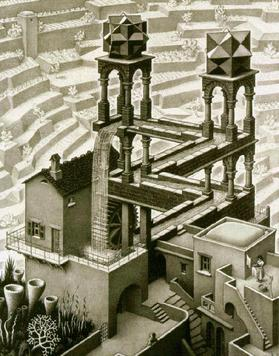
\includegraphics[height=0.7\textheight]{graphics/escher_low}\\
  \grau{\footnotesize M.\,C.\ Escher, \textit{Wasserfall}, Lithografie, 1961.\\
  \url{https://en.wikipedia.org/wiki/File:Escher_Waterfall.jpg}}
\end{frame}

\begin{frame}
  {Das war die Vorbereitung}
  \onslide<+->
  \onslide<+->
  \centering 
  Sie sind jetzt bereit für den schönsten Lexikoneintrag überhaupt!\\
  \Doppelzeile
  \onslide<+->
  \scalebox{1.5}{%
    \begin{avm}
      \[
        phon & \<\> \\
        loc  & \@1 \[ cat|head|dsl & \@1 \]
      \]
    \end{avm}
  }
\end{frame}

\begin{frame}
  {Satzsyntax, und zwar auch noch deutsche!}
  \onslide<+->
  \onslide<+->
  Über Konstituentenstellung müssen wir sowieso noch reden!\\
  \Zeile
  \begin{itemize}[<+->]
    \item .
  \end{itemize}
  \Zeile
  \onslide<+->
  \centering 
  \grau{\citet[Kapitel~9]{MuellerLehrbuch3}}\\
\end{frame}

\begin{frame}
  {Scrambling}
\end{frame}

\begin{frame}
  {Linearisierungsregeln}
\end{frame}

\begin{frame}
  {Links- und Rechtsköpfigkeit}
\end{frame}

\section{Verbbewegung}

\begin{frame}
  {Wiederholung | Bewegungstransformationen}
  \onslide<+->
  \onslide<+->
  \alert{Bewegung} | Erklärt \alert{Abhängigkeiten} zwischen Positionen in Strukturen.\\
  \grau{\footnotesize\textit{Transformationen} sagt man seit der GB-Theorie nicht mehr. Technisch gesehen sind es Transformationen.}\\
  \onslide<+->
  \Zeile
  \centering
  \begin{tabular}{cc}
    \scalebox{0.8}{\begin{forest}
      [CP
        [C$'$
          [C
            [\it dass, rottree]
          ]
          [VP
            [NP
              [\it Matthias, bluetree]
            ]
            [V$'$
              [NP
                [\it Doro]
              ]
              [V
                [\it besucht, gruentree]
              ]
            ]
          ]
        ]
      ]
    \end{forest}} & %
    \visible<4->{\scalebox{0.8}{\begin{forest}
      [CP
        [NP
            [\it Matthias\Sub{2}, bluetree, name=Matthias]
        ]
        [C$'$
          [C
            [\it besucht\Sub{1}, gruentree, name=besucht]
          ]
          [VP
            [t\Sub{2}, bluetree, name=t2]
            [V$'$
              [NP
                [\it Doro]
              ]
              [V
                [t\Sub{1}, gruentree, name=t1]
              ]
            ]
          ]
        ]
      ]
      {\draw [<->, bend left=70, gruen, thick] (t1.south) to (besucht.south);}
      {\draw [<->, bend left=70, trueblue, thick] (t2.south) to (Matthias.south);}
    \end{forest}}} \\
  \end{tabular}
\end{frame}


\begin{frame}
  {Wiederholung | Theorien ohne Transformationen im weiteren Sinn}
  \onslide<+->
  \onslide<+->
  HPSG | \alert{Die gleichen Abhängigkeiten ohne Bewegung}, dafür mit \alert{Strukturteilung}\\
  \grau{\footnotesize Aber nicht unbedingt ohne leere Elemente.}\\
  \onslide<+->
  \Zeile
  \centering 
  \begin{tabular}[h]{cp{0.05\textwidth}c}
    \scalebox{0.6}{\begin{forest}
      [ VP
        [NP
          [\it \alt<1-4|handout:0>{Matthias}{\alert{Matthias\Sub{1}}}]
        ]
        [VP
          [V
            [\it \alt<1-4|handout:0>{besucht}{\gruen{besucht\Sub{2}}}]
          ]
          [VP
            [NP
              [\it Doro]
            ]
            [V
              [\alt<1-4|handout:0>{$\emptyset$}{\alert{t\Sub{1}}}]
              [\alt<1-4|handout:0>{$\emptyset$}{\gruen{t\Sub{2}}}]
            ]
          ]
        ]
      ]
    \end{forest}} && % 
    \onslide<+->\alt<1-4|handout:0>{%
    \scalebox{0.55}{\begin{avm}
      \[ phon & \phon{Matthias, besucht, Doro} \\
        non-hd-dtr & \[ phon & \phon{Matthias} \] \\
        hd-dtr & \[ phon & \phon{besucht, Doro} \\
          hd-dtr & \[ phon & \phon{besucht} \] \\
          non-hd-dtr & \[ phon & \phon{Doro} \\
            non-hd-dtr & \[ phon & \phon{Doro} \] \\
            hd-dtr & \[ phon & \<\> \\
              non-hd-dtr & \[ phon & \<\> \] \\
              hd-dtr & \[ phon & \<\> \]
            \]
          \]
        \]
      \]
    \end{avm}}}{%
    \scalebox{0.55}{\begin{avm}
      \[ phon & \phon{Matthias, besucht, Doro} \\
        non-hd-dtr & \alert{\[ phon & \phon{Matthias } \\ 
          magical-features & \@1
        \]} \\
        hd-dtr & \[ phon & \phon{besucht, Doro} \\
          hd-dtr & \gruen{\[ phon & \phon{besucht} \\
          magical-features & \@2 \]} \\
          non-hd-dtr & \[ phon & \phon{Doro} \\
            non-hd-dtr & \[ phon & \phon{Doro} \] \\
            hd-dtr & \[ phon & \<\> \\
              non-hd-dtr & \alert{\[ phon & \<\> \\
              magical-features & \@1 \]} \\
              hd-dtr & \gruen{\[ phon & \<\> \\
              magical-features & \@2 \]}
            \]
          \]
        \]
      \]
    \end{avm}}%
    }\\
  \end{tabular}  \\
  \Zeile
  \onslide<+->
  \onslide<+->
  \gruen{Heute klären wir für das bewegte Verb, wie die Merkmalsmagie funktioniert.}\\
\end{frame}

\begin{frame}
  {Nicht streng lokale Theorien}
  \onslide<+->
  \onslide<+->
  Auch bei \textit{Bewegung} geht es letztlich darum, wie die magischen Merkmale\\
  in der Struktur einander zugeordnet werden können.\\
  \onslide<+->
  \Zeile
  \begin{minipage}{0.35\textwidth}
    \centering 
    \scalebox{0.8}{\begin{forest}
      [CP
        [NP
            [\it Matthias\Sub{2}, bluetree, name=Matthias]
        ]
        [C$'$
          [C
            [\it besucht\Sub{1}, gruentree, name=besucht]
          ]
          [VP
            [t\Sub{2}, bluetree, name=t2]
            [V$'$
              [NP
                [\it Doro]
              ]
              [V
                [t\Sub{1}, gruentree, name=t1]
              ]
            ]
          ]
        ]
      ]
      {\draw [<->, bend left=70, gruen, thick] (t1.south) to (besucht.south);}
      {\draw [<->, bend left=70, trueblue, thick] (t2.south) to (Matthias.south);}
    \end{forest}}
  \end{minipage}\hspace{1em}\begin{minipage}{0.6\textwidth}
    Probleme\\
    \Halbzeile
    \begin{itemize}[<+->]\small
      \item Koindizierte bewegte Elemente und Spuren müssen eine Kette (\textit{chain}) bilden.
      \item Dazu muss der Formalismus sie einander zuordnen.
      \item Aus Sicht des bewegten Elements muss \rot{die gesamte c"=Kommando"=Domäne durchsucht werden}.
      \item Der Baum kann beliebig komplex sein, es gibt kein einfaches Rezept für die Suche (in der Art von: \textit{aufwärts, dann abwärts: rechts, rechts, links}).
      \item \rot{Bäume} und \rot{Baumdurchsuchungen} machen solche Theorien unnötig komplex.
    \end{itemize}
  \end{minipage}
\end{frame}

\begin{frame}
  {Streng lokale Theorien}
  \onslide<+->
  \onslide<+->
  In einer lokalen Theorie müssen die relevanten Informationen\\
  \alert{am jeweiligen "`Knoten"' verfügbar sein}. Man durchsucht keine Bäume!\\
  \onslide<+->
  \Viertelzeile
  Die Information, dass etwas fehlt, wird an geeigneter Stelle \alert{von Knoten zu Knoten weitergegeben}. Hier steht hinter dem \alert{Doubleslash} jeweils, was fehlt.\\
  \centering 
  \onslide<+->
  \Halbzeile
  \centering
    \scalebox{0.8}{\begin{forest}
        [VP
          [V
            [\it besucht]
          ]
          [VP//V
            [NP
              [\it Matthias]
            ]
            [V$'$//V
              [NP
                [\it Doro]
              ]
              [\gruen<5->{V//V}
              ]
            ]
          ]
        ]
      \end{forest}}\onslide<+->\hspace{3em}\scalebox{0.8}{%
    \gruen{\raisebox{-4.5\baselineskip}{\begin{avm}
      \[
        phon & \<\> \\
        loc  & \@1 \[ cat|head|dsl & \@1 \]
      \]
    \end{avm}
  }}}
\end{frame}

\begin{frame}
  {Ausblick auf die Modellierung}
  \onslide<+->
  Um \alert{Verbbewegung} zu modellieren, brauchen wir keine neuen Regeln, sondern:\\
  \Halbzeile
  \begin{enumerate}[<+->]
    \item Eine Zusammenfassung von \textsc{cat} und \textsc{cont} zu \alert{\textsc{local}} bzw.\ \alert{\textsc{loc}}.
    \Viertelzeile
    \item Eine \alert{lexikalische Verbspur} für alle Verben
      \begin{itemize}[<+->]
        \item Ihr \textsc{phon} ist eine leere Liste.
        \item Ihr Kopfmerkmal \textsc{Doubleslash} bzw.\ \alert{\textsc{dsl} ist strukturgeteilt mit ihrem \textsc{loc}}.
        \item Mit \textsc{dsl} kodiert sie, was fehlt (also das lexikalische Verb selbst).
        \item Sie ist \textsc{initial $-$} wie normale Verben.
        \item Als Kopfmerkmal wird \textsc{head|dsl} in Kopf-Strukturen weitergegeben.
      \end{itemize}
      \Viertelzeile
    \item Einen Lexikoneintrag per \alert{Lexikonregel für das bewegte Verb}
      \begin{itemize}[<+->]
        \item Sein \textsc{phon} entspricht dem seiner \textsc{lex-dtr} (normales Verb).
        \item Er ist \textsc{initial $+$}, weil er links von der VP steht.
        \item Auf seiner \textsc{subcat} steht eine VP, deren \textsc{loc|cat|head|dsl} \ldots
        \item \ldots\ mit dem \textsc{loc} seiner \textsc{lex-dtr} token-identisch ist.
        \item \gruen{Dadurch wird die gesamte Syntax und Semantik des lexikalischen Verbs\\
          durch die Knoten, deren Kopf die Verbspur ist, in die Verbspur gepumpt.}
        \item \orongsch{Die Verbspur muss daher nicht verbspezifisch sein!}
      \end{itemize}
  \end{enumerate}
\end{frame}

\newcommand{\AvmGa}{%
  \scalebox{0.5}{\begin{avm}
    \[ \asort{word} 
      phon & \<\> \\
      loc & \@1 \[cat|head & \@5 \[dsl & \@1 \]\]
    \]
  \end{avm}}
}

\newcommand{\AvmGb}{%
  \scalebox{0.5}{\begin{avm}
    \@3 \[ \asort{word}
      phon & \phon{hustet} \\
        loc & \@1 \[cat & \[
          head|initial & $-$ \\
          subcat & \<\@2 \[
            loc|cat & \[
              head & \textit{\sl noun} \\
              subcat & \<\> \\
            \]
          \]\>
        \]
      \]
    \]
  \end{avm}}
}

\newcommand{\AvmGc}{%
  \scalebox{0.5}{\begin{avm}
    \[ \asort{v1-lex-rule} 
      phon & \phon{hustet} \\
      loc|cat & \[
        head|initial & $+$ \\
        subcat & \<
          \@4 \[
            loc|cat & \[
              head|dsl & \@1 \\
              subcat & \<\> \\
            \]
          \]
        \>\\
      \]\\
      lex-dtr & \@3 \\
    \]
  \end{avm}}
}

\newcommand{\AvmGd}{%
  \scalebox{0.5}{\begin{avm}
    \@2 \[ \asort{word} 
      phon & \phon{Matthias} \\
    \]
  \end{avm}}
}

\newcommand{\AvmGe}{%
  \scalebox{0.5}{\begin{avm}
    \@4 \[ \asort{hd-arg-phr} 
           phon & \phon{Matthias}$\oplus$\<\> \\
           loc|cat|head & \@5 \[dsl & \@1 \] \\
    \]
  \end{avm}}
}

\newcommand{\AvmGf}{%
  \scalebox{0.5}{\begin{avm}
    \[ \asort{hd-arg-phr}
      phon & \phon{hustet,Matthias}$\oplus$\<\> \\
    \]
  \end{avm}}
}

\begin{frame}
  {Analyse (ausnahmsweise als Baum)}
  \onslide<+->
  \onslide<+->
  \alert{V1-Satz} | \textit{Hustet Matthias?} \\
  \onslide<+->
  \centering
  \begin{forest}
    [\AvmGf
      [\AvmGc
        [\AvmGb]
      ]
      [\AvmGe
        [\AvmGd]
        [\AvmGa]
      ]
    ]
  \end{forest}
\end{frame}


\section{Details der Analyse}

\begin{frame}
  {Neue Merkmalgeometrie für Zeichen}
  \onslide<+->
  \onslide<+->
  \centering 
  \begin{avm}
    \[
      \asort{sign}
      phon & \textit{\sl list of phoneme strings} \\
      \grau{synsem} & \[
        loc & \[
          cat & \[
            head & \textit{\sl head}\\
            subcat & \textit{\sl list of signs} \\
          \] \\
          cont & \textit{\sl cont} \\
        \]\\
        \grau{nonloc} & \grau{\textit{\sl non-local}} \\
      \]
    \]
  \end{avm}\\
  \onslide<+->
  \Zeile
  \textsc{nonloc} brauchen wir nächste Woche.\\
  \onslide<+->
  \textsc{synsem} brauchen wir bei der Lektüre von \citet{ps2}.
\end{frame}

\begin{frame}
  {Lexikonregel für Verben in Nicht-Letzt-Stellung}
  \onslide<+->
  \onslide<+->
  Bildet eine Verb wie \textit{hustet}, das eine VP verlangt, in der es selbst "`fehlt"'.\\
  \onslide<+->
  \Zeile
  \centering 
  \begin{avm}
    \[ loc|cat & \[
      head & \[ \asort{verb}
        initial & $+$ \\
      \] \\
      subcat & \<
        \[ loc|cat & \[
          head & \[ \asort{verb} dsl & \gruen{\@1} \] \\
          subcat & \<\> \\
        \]
      \]
      \> \\
    \]\\
      lex-dtr & \[
        loc & \gruen{\@1} \[
        cat|head & \[
          \asort{verb}
          vform & fin \\
          initial & $-$ \\
        \]
      \]
      \]
    \]
  \end{avm}
\end{frame}

\begin{frame}
  {Verbot nicht-stummer Spuren}
  \onslide<+->
  \onslide<+->
  Verhindert ansonsten mögliche Verbdopplung | \textit{\rot{*Hustet Matthias hustet?}}\\
  \onslide<+->
  \Zeile
  \centering 
  \begin{avm}
    \[ hd-dtr & \[ \asort{word} phon & \textit{\sl non-empty-list} \] \]
  \end{avm}\raisebox{-0.75\baselineskip}{$\Rightarrow$%
  \begin{avm}
    \[ loc|cat|head|dsl & \textit{\sl none} \]
  \end{avm}}
\end{frame}




\newcommand{\AvmGSema}{%
  \scalebox{0.44}{\begin{avm}
    \[ \asort{word} 
      phon & \<\> \\
      loc & \@1 \[
        cat|head & \@5 \[dsl & \@1 \] \\
        cont & \@7 \\
    \]
    \]
  \end{avm}}
}

\newcommand{\AvmGSemb}{%
  \scalebox{0.44}{\begin{avm}
    \@3 \[ \asort{word}
      phon & \phon{besucht} \\
        loc & \@1 \[cat & \[
          head|initial & $-$ \\
          subcat & \<\@2 NP\UpSub{\sl Nom}{\@{10}}, \@6 NP\UpSub{\sl Acc}{\@{11}}\>
        \] \\
        cont & \@7 \[ restr & \< \[ \asort{visit-rel} agent & \@{10} \\ other & \@{11} \] \> \] \\
      \]
    \]
  \end{avm}}
}

\newcommand{\AvmGSemc}{%
  \scalebox{0.44}{\begin{avm}
    \[ \asort{v1-lex-rule} 
      phon & \phon{besucht} \\
      loc|cat & \[
        head|initial & $+$ \\
        subcat & \<
          \@4 \[
            loc|cat & \[
              head|dsl & \@1 \\
              subcat & \<\> \\
            \]
          \]
        \>\\
      \]\\
      lex-dtr & \@3 \\
    \]
  \end{avm}}
}

\newcommand{\AvmGSemd}{%
  \scalebox{0.44}{\begin{avm}
    \@2 \[ \asort{word} 
      phon & \phon{Matthias} \\
      loc|cont|ind & \@{10} \\
    \]
  \end{avm}}
}

\newcommand{\AvmGSemdd}{%
  \scalebox{0.44}{\begin{avm}
    \@6 \[ \asort{word} 
      phon & \phon{Doro} \\
      loc|cont|ind & \@{11} \\
    \]
  \end{avm}}
}

\newcommand{\AvmGSeme}{%
  \scalebox{0.44}{\begin{avm}
    \@4 \[ \asort{hd-arg-phr} 
           phon & \phon{Matthias,Doro}$\oplus$\<\> \\
           loc & \[
             cat & \[
               head & \@5 \[dsl & \@1 \] \\
               subcat & \<\> \\
             \] \\
             cont & \@7 \\
           \]\\
    \]
  \end{avm}}
}

\newcommand{\AvmGSemee}{%
  \scalebox{0.44}{\begin{avm}
    \@4 \[ \asort{hd-arg-phr} 
           phon & \phon{Doro}$\oplus$\<\> \\
           loc & \[
             cat & \[
               head & \@5 \[dsl & \@1 \] \\
               subcat & \<\@2\>
             \] \\
             cont & \@7 \\
           \] \\
    \]
  \end{avm}}
}

\newcommand{\AvmGSemf}{%
  \scalebox{0.44}{\begin{avm}
    \[ \asort{hd-arg-phr}
      phon & \phon{besucht,Matthias,Doro}$\oplus$\<\> \\
      cont & \@7 \\
    \]
  \end{avm}}
}

\begin{frame}
  {Die Semantik gibt es umsonst!}
  \onslide<+->
  \onslide<+->
  \centering
  \vspace{-1.75\baselineskip}
  \begin{forest}
    [\AvmGSemf
      [\AvmGSemc
        [\AvmGSemb]
      ]
      [\AvmGSeme
        [\AvmGSemd]
        [\AvmGSemee
          [\AvmGSemdd]
          [\AvmGSema]
        ]
      ]
    ]
  \end{forest}
\end{frame}



\section{Nächste Woche}

\begin{frame}
  {Vorbereitung}
  \onslide<+->
  \onslide<+->
  \centering 
  \large
  Nächste Woche reden wir über Fernabhängigkeiten wie Vorfeldbesetzung.\\
  \onslide<+->
  \Zeile
  \rot{Sie sollten dringend vorher aus dem HPSG-Buch\\
  von Kapitel 10 die Seiten 163--171 lesen!}\\
  \onslide<+->
  \Viertelzeile
  Das sind \gruen{9} Seiten.\\
\end{frame}

  \let\subsection\section\let\section\woopsi

  \section{Nichtlokale Abhängigkeiten}
  \let\woopsi\section\let\section\subsection\let\subsection\subsubsection
  \input{includes/08.+Nichtlokale+Abhängigkeiten.tex}
  \let\subsection\section\let\section\woopsi

  \section{Quantorenspeicher}
  \let\woopsi\section\let\section\subsection\let\subsection\subsubsection
  \section{Einleitung}

\begin{frame}
  {Determinierer und Quantifikation}
  \onslide<+->
  \onslide<+->
  Bisher haben wir nur indefinite NPs modelliert.\\
  \Zeile
  \begin{itemize}[<+->]
    \item x
  \end{itemize}
  \Zeile
  \onslide<+->
  \centering 
  \grau{\citet[47--59]{ps2}}\\
\end{frame}


\section{Nächste Woche}

\begin{frame}
  {Vorbereitung}
  \onslide<+->
  \onslide<+->
  \centering 
  \large
  Nächste Woche reden wir über Unterspezifikationssemantik.\\
  \onslide<+->
  \Zeile
  \rot{Sie sollten dringend vorher aus \citet{CFPS2005a}\\
  die Seiten 281--291 und 304--311 lesen (s.~Webseite)!}\\
  \onslide<+->
  \Viertelzeile
  Das sind \rot{18} Seiten.\\
\end{frame}

  \let\subsection\section\let\section\woopsi

  \section{Unterspezifikation}
  \let\woopsi\section\let\section\subsection\let\subsection\subsubsection
  \section{Einleitung}

\begin{frame}
  {Warum sollte man Quantorenskopus auflösen?}
  \onslide<+->
  \onslide<+->
  Wir können sie Semantik auch unterspezifiziert lassen.\\
  \Zeile
  \begin{itemize}[<+->]
    \item x
  \end{itemize}
  \Zeile
  \onslide<+->
  \centering 
  \grau{\citet{CFPS2005a}}\\
\end{frame}

\begin{frame}
  {Vorbereitung}
  \onslide<+->
  \onslide<+->
  \centering 
  \large
  Nächste Woche bekommen Sie einen Einblick in die formalen Grundlagen.\\
  \onslide<+->
  \Zeile
  \rot{Sie \textbf{müssen} dazu aus \citet{Richter2021a}\\
  die Seiten 89--100 lesen (s.~Link auf Webseite)!}\\
  \onslide<+->
  \Viertelzeile
  Das sind \gruen{11} Seiten.\\
\end{frame}

  \let\subsection\section\let\section\woopsi

\fi


\makeatletter
\setcounter{lastpagemainpart}{\the\c@framenumber}
\makeatother

\appendix

\begin{frame}[allowframebreaks]
  {Literatur}
  \renewcommand*{\bibfont}{\footnotesize}
  \setbeamertemplate{bibliography item}{}
  \printbibliography
\end{frame}

\begin{frame}
  {Autor}
  \begin{block}{Kontakt}
    Prof.\ Dr.\ Roland Schäfer\\
    Institut für Germanistische Sprachwissenschaft\\
    Friedrich-Schiller-Universität Jena\\
    Fürstengraben 30\\
    07743 Jena\\[\baselineskip]
    \url{https://rolandschaefer.net}\\
    \texttt{roland.schaefer@uni-jena.de}
  \end{block}
\end{frame}

\begin{frame}
  {Lizenz}
  \begin{block}{Creative Commons BY-SA-3.0-DE}
    Dieses Werk ist unter einer Creative Commons Lizenz vom Typ \textit{Namensnennung - Weitergabe unter gleichen Bedingungen 3.0 Deutschland} zugänglich.
    Um eine Kopie dieser Lizenz einzusehen, konsultieren Sie \url{http://creativecommons.org/licenses/by-sa/3.0/de/} oder wenden Sie sich brieflich an Creative Commons, Postfach 1866, Mountain View, California, 94042, USA.
  \end{block}
\end{frame}

\mode<beamer>{\setcounter{framenumber}{\thelastpagemainpart}}

\end{document}
